\documentclass[journal]{IEEEtran}
\IEEEoverridecommandlockouts
% The preceding line is only needed to identify funding in the first footnote. If that is unneeded, please comment it out.
\usepackage{cite}
\usepackage{amsmath,amssymb,amsfonts}
\usepackage{color}
\usepackage{algorithmic}
% \usepackage[ruled,vlined]{algorithm2e}
\usepackage{graphicx}
\usepackage{textcomp}
\def\BibTeX{{\rm B\kern-.05em{\sc i\kern-.025em b}\kern-.08em
    T\kern-.1667em\lower.7ex\hbox{E}\kern-.125emX}}

\hyphenation{op-tical net-works semi-conduc-tor}

\newcommand{\setX}{\mathbf{X}}
\newcommand{\sx}{\mathbf{x}}

\begin{document}

\title{Extended Target Poisson Multi-Bernoulli Filter\\
% {\footnotesize \textsuperscript{*}Note: Sub-titles are not captured in Xplore and
% should not be used}
% \thanks{Identify applicable funding agency here. If none, delete this.}
}

% \author{\IEEEauthorblockN{1\textsuperscript{st} Yuxuan Xia}
% \IEEEauthorblockA{\textit{Department of Electrical Engineering} \\
% \textit{Chalmers University of Technology}\\
% G\"{o}teborg, Sweden \\
% yuxuanx@student.chalmers.se}
% \and
% \IEEEauthorblockN{2\textsuperscript{nd} Karl Granstr\"{o}m}
% \IEEEauthorblockA{\textit{Department of Electrical Engineering} \\
% \textit{Chalmers University of Technology}\\
% G\"{o}teborg, Sweden \\
% karl.granstrom@chalmers.se}
% \and
% \IEEEauthorblockN{3\textsuperscript{rd} Lennart Svensson}
% \IEEEauthorblockA{\textit{Department of Electrical Engineering} \\
% \textit{Chalmers University of Technology}\\
% G\"{o}teborg, Sweden \\
% lennart.svensson@chalmers.se}
% }
% \author{\IEEEauthorblockN{Yuxuan Xia\IEEEauthorrefmark{2},
% Karl Granstr\"{o}m\IEEEauthorrefmark{2},
% Lennart Svensson\IEEEauthorrefmark{2}, 
% Maryam Fatemi\IEEEauthorrefmark{3}}
% \IEEEauthorblockA{\IEEEauthorrefmark{2}Department of Electrical Engineering, Chalmers University of Technology, G\"{o}teborg, Sweden}
% \IEEEauthorblockA{\IEEEauthorrefmark{3}Zenuity, G\"{o}teborg, Sweden}
% }

\author{Yuxuan~Xia, Karl~Granstr\"{o}m,~\IEEEmembership{Member,~IEEE,} Lennart~Svensson,~\IEEEmembership{Senior~Member,~IEEE,} and Maryam Fatemi% <-this % stops a space
\thanks{Yuxuan Xia is with Chalmers University of Technology, G\"{o}teborg, Sweden. E-mail: \texttt{yuxuanx@student.chalmers.se}}% <-this % stops a space
\thanks{Karl Granstr\"{o}m and Lennart Svensson are with the Department of Electrical Engineering, Chalmers University of Technology, G\"{o}teborg, Sweden.
E-mail: \texttt{firstname.lastname@chalmers.se}}% <-this % stops a space
\thanks{Maryam Fatemi is with Zenuity, G\"{o}teborg, Sweden. E-mail: \texttt{maryam.fatemi@zenuity.com}}}

\maketitle

\begin{abstract}
In this paper, a Poisson multi-Bernoulli (PMB) filter for multiple extended targets estimation is presented. The PMB filter is based on the Poisson multi-Bernoulli mixture (PMBM) conjugate prior and approximates the multi-Bernoulli mixture (MBM) in the posterior as a single multi-Bernoulli. By only having a single multi-Bernoulli representing detected targets in the posterior, the computational cost due to the data association problem can be effectively reduced. Different methods to merge the MBM are presented, along with their gamma Gaussian inverse Wishart implementations. The performance of the PMB filter is compared to the PMBM filter in different simulated scenarios. 
\end{abstract}

\begin{IEEEkeywords}
Multiple target tracking, extended target, random matrix model, random finite sets, Bayesian estimation, variational inference
\end{IEEEkeywords}

\section{Introduction}
% The development of autonomous driving has attracted an enormous amount of interest in research during last decades. In order for an autonomous vehicle to be deployed in real-world environments, it must be capable of reliably and efficiently modelling static as well as dynamical obstacles, e.g., landmarks, pedestrians and other nearby moving vehicles. 
Multiple target tracking (MTT) is the process of estimating the set of target trajectories based on a sequence of noise-corrupted measurements, including missed detections and false alarms \cite{mtt}. Traditionally, MTT algorithms have been tailored to the ``point target'' assumption: each target is modelled as a point without spatial extent, and each target gives rise to at most one measurement per time scan. However, modern high-resolution radar and lidar sensors make the “point target” assumption unrealistic, because with such sensors it is common that a target gives rise to multiple measurements per time scan. The tracking of such a target leads to the so-called extended target tracking problem, where the objective is to recursively determine the extent and kinematic parameters of the targets over time. A detailed overview of extended target tracking literature is given in \cite{extendedoverview}. In this paper, we focus on the estimation of the current set of targets, which is called multiple target filtering\footnote{The ultimate output from an MTT algorithm is a set of target trajectories, i.e., a set of target state sequences. The ability to maintain target trajectories over time is outside the scope of this paper.}. 

Random Finite Sets (RFS) \cite{rfs} is a popular and widely used framework that facilitates an elegant Bayesian formulation of the MTT problem. In the early stage, RFS-based MTT approaches were developed based on moment approximations of posterior multi-target densities, including the Probability Hypothesis Density (PHD) filter \cite{phdpoint,phdextended2,phdextended3} and the Cardinalised PHD (CPHD) filter \cite{cphdpoint,cphdextended}. In recent years, a significant trend in RFS-based MTT is the development of conjugate multi-target distributions, meaning that the posterior multi-target distribution has the same functional form as the prior. 

Two types of MTT conjugate priors can be found in the literature: the $\delta$-Generalized Labelled Multi-Bernoulli ($\delta$-GLMB) \cite{glmbconjugateprior} and the Poisson Multi-Bernoulli Mixture (PMBM) \cite{pmbmpoint}. In the $\delta$-GLMB conjugate prior, labels are added to target states facilitating the forming of target trajectories \cite{glmbconjugateprior}. In the PMBM conjugate prior, the set of targets is separated into two disjoint and independent subsets: targets that have been detected, and targets that have not been detected \cite{pmbmpoint}. The differences between representing the multi-target state density in the PMBM form and the $\delta$-GLMB form are discussed in \cite{pmbmpoint2}. Simulation results have shown that the PMBM filter \cite{pmbmpoint,pmbmpoint2,pmbmextended,pmbmextended2} outperforms the $\delta$-GLMB filter \cite{glmbpoint,lmbextended} for both point \cite{performanceevaluation} and extended \cite{pmbmextended2} target filtering. 

% Solving the MTT problem is complicated by the unknown correspondence between targets and measurements, known as data association. 
Data association is an inherent problem of MTT. Because each target can generate multiple measurements per time scan, the problem of data association is even more challenging in multiple extended target tracking, than it in multiple point target tracking. The PHD and the CPHD filters avoid handling the data association uncertainty explicitly by moment approximation\footnote{In the extended PHD/CPHD filter, different partitions of the set of measurements have to be computed in prior to moment approximation.}, however, comparisons have shown that PHD and CPHD filters have worse tracking performance, compared to MTT conjugate priors \cite{lmbextended,pmbmextended2}. Filters based on conjugate priors provide more accurate approximations to the exact posterior distributions, however, due to the unknown number of data associations, the number of multi-Bernoulli (MB) components in the posterior density of the $\delta$-GLMB and the PMBM filters grow rapidly as more data is observed. Different approximation methods can be used to keep the number of MBs at a tractable level, see \cite{glmbpoint,pmbmpoint2} for point target filtering, and \cite{lmbextended,pmbmextended,pmbmextended2} for extended target filtering. The main advantage of using conjugate prior in MTT, instead of moment approximations, is that the posterior distribution can be approximated arbitrarily well as long as sufficient parameters are used. 

Simulation studies have shown that RFS methods based on MTT conjugate priors all outperform RFS methods based on moment approximations, see performance comparison \cite{glmbpoint,lmb,pmbmpoint2} on point target filtering and \cite{lmbextended,pmbmextended,pmbmextended2} on extended target filtering. The computational cost of the PMBM and $\delta$-GLMB filters can be greatly reduced by approximating the MB mixture (MBM) in the posterior as a single MB. For example, the labelled MB (LMB) filter is an efficient approximation of the $\delta$-GLMB filter, proposed in \cite{lmb} for point target and in \cite{lmbextended} for extended target. Similarly, approximating the PMBM posterior as a single MB leads to the so-called Poisson MB (PMB) filter. Different variants of the PMB filter have been developed for point target filtering \cite{pmbmpoint,variational}, among which the variational MB algorithm \cite{variational} provides the most accurate target state estimation. 

A performance evaluation of filters based on different MB conjugate priors for point target estimation, given in \cite{performanceevaluation}, has shown that the PMB filter has very promising performance regarding estimation error and computational time. It is therefore of interest to develop a PMB filter for extended targets. In this paper, we develop several different extended target PMB filters, and compare them to the extended target PMBM filter. 

The contributions are summarized as follows:

% Compared to the point target PMB filter, a considerable difficulty in designing an extended target PMB filter is to accurately estimate the states of potential targets that are detected for the first time. 
% In this paper, we develop several different extended target PMB filters, and compare them to the extended target PMBM filter. The contributions are summarized as follows:

% The variational MB filter finds the best-fitting MB by approximating the true posterior MBM with the MB that minimizes the Kullback-Leibler (KL) divergence. A performance evaluation of filters based on MB conjugate prior for point target estimation given in \cite{performanceevaluation} has shown that the PMB filter with variational approximation has the best overall performance regarding estimation error and computational time. 



% The main contribution of this paper is presenting different versions of the PMB filter for multiple extended target filtering, along with their GGIW implementations. The pros and cons of the different PMB versions are discussed, and they are compared in an extensive simulation study. Two different implementations of the variational MB algorithm for merging MBM describing already detected targets are studied, one is based on the efficient approximation of feasible set proposed in \cite{variational}, and the other is based on optimal assignment following a similar optimization procedure used by the set joint probabilistic data association (SJPDA) filter \cite{sjpda}. They are compared to the track-oriented PMB filter, which is adapted from the track-oriented marginal MeMBer-Poisson (TOMB/P) filter \cite{pmbmpoint} for point targets, and the PMBM filter. In addition, we propose a method to create new tracks in the extended PMB filter in a reasonable way. 

% The paper is organized as follows. Background on multiple extended target tracking and PMBM conjugate prior is introduced in Section II. The problem formulation is given in Section III. Different versions of the PMB filter are presented in Section IV and V. The GGIW implementations are presented in Section VI, and simulation results are presented in Section VII.

% This paper contains the following contributions:
\begin{enumerate}
    \item In Section V, we present the track-oriented PMB (TO-PMB) filter, which is an adaptation of the track-oriented marginal MeMBer-Poisson (TOMB/P) filter \cite{pmbmpoint} for point targets. We also analyze the drawback of this track-oriented merging approach, and highlight the challenges in forming new tracks in the extended target PMB filter.
    \item In Section VI, we present a variational MB filter that considers the forming of pre-existing and new tracks separately. We first apply the variational MB algorithm \cite{variational} to form pre-existing tracks, then we use related ideas to propose a greedy method to form new tracks. Two different implementations of the variational MB algorithm are studied, one is based on the efficient approximation of the feasible set, proposed in \cite{variational}, and the other is based on the most likely assignment, following a similar optimization procedure used by the set joint probabilistic data association (SJPDA) filter \cite{sjpda}. 
    \item In Section VII, we present implementations of the PMB filters for a common extended target model. 
    \item In Section VIII, different variants of the PMB filter are compared to the PMBM filter in an extensive simulation study. 
\end{enumerate}
In Section II, we give some background on Bayesian multi-target filtering, RFS modelling, the PMBM conjugate prior and some RFS mixture reduction techniques. In Section III, we present the problem formulation. In Section IV, we present the extended target PMB filter recursion. Nomenclature is presented in Table \ref{tab:notations}. 


\section{Background}
In this section, we first give introductions to Bayesian filtering and RFS modelling. Next, we present the PMBM conjugate prior for multiple extended target filtering. In addition, we describe techniques on how to approximate a mixture of Bernoulli RFSs and an MBM, respectively, in the sense of minimizing the Kullback-Leibler (KL) divergence.

% After that, we give an introduction to different variants of the point target PMB filter. The extended target PMB filter is inspired by, and adapted from, the point target counterpart. Thus, giving an overview of the point target PMB filter will facilitate the presentation of the extended target PMB filter.

\begin{table}[!t]
\footnotesize
\caption{Nomenclature}
\label{tab:notations}
\centering
% \resizebox{\textwidth}{!}{%
\begin{tabular}{l}
  \hline
  \begin{minipage}{0.45\textwidth}
    \vskip 1pt
    \begin{itemize}
    \item $\langle a,b\rangle=\int a(x)b(x)dx$: inner product of $a(x)$ and $b(x)$.
    \item $|V|$: determinant of matrix $V$.
    \item $|\mathbf{X}|$: cardinality of set $\mathbf{X}$.
   \item $\Pi_N$: set of permutation functions on $I_N \triangleq \{1,...,N\}$
   $$\Pi_N = \{\pi:I_N\rightarrow I_N|i\neq j\Rightarrow \pi(i)\neq\pi(j)\}.$$
   \item $\uplus$: disjoint set union, i.e., $Y\uplus U=X$ means that $Y\cup U=X$ and $Y\cap U=\emptyset$.
   \item $D_{\text{KL}}(p||q)=\int p(x)\log\big(\frac{p(x)}{q(x)}\big)dx$: Kullback-Leibler divergence between $p(x)$ and $q(x)$.
   \item $\Gamma_d(\cdot)$: multivariate gamma function.
   \item $\varphi_0(\cdot)$: digamma function.
   \item $\text{Tr}(X)$: trace of matrix $X$.
   \item $\text{I}_m$: identity matrix of size $m\times m$.
   \item $\mathcal{GAM}(\gamma;a,b)$: probability density function of gamma distribution defined on $\gamma > 0$ with shape $a$ and rate $b$.
   \item $\mathcal{IW}_d(\chi;v,V)$: probability density function of inverse-Wishart distribution defined on positive definite $d\times d$ matrix with degrees of freedom $v$ and $d\times d$ scale matrix $V$.
   \end{itemize}
   \vskip 1pt
 \end{minipage}
 \\
  \hline
 \end{tabular}
\end{table}

\subsection{Bayesian multi-target filtering}

In RFS-based MTT methods, target states and measurements are represented in the form of finite sets. Let $\mathbf{x}_k$ denote the single target state at discrete time step $k$, and let $\mathbf{X}_k$ denote the target set. In extended target tracking, the target state models both the kinematic properties, and the extent, of the target. The target set cardinality $|\mathbf{X}_k|$ is a time-varying discrete random variable, and each target state $\mathbf{x}_k\in\mathbf{X}_k$ is also a random variable. Let $\mathbf{z}^m_k$ denote the $m$th measurement at discrete time step $k$. The set of measurements obtained at time step $k$ is denoted as $\mathbf{Z}_k$, including clutter and target-generated measurements with unknown origin. The sequence of all the measurement sets received so far up to time step $k$ is denoted as $\mathbf{Z}^k$.

% The objective of multiple target filtering is to estimate the set of targets $\mathbf{X}_k$, including the number of targets and individual target state, using the information contained in the measurement set sequence $\mathbf{Z}^k$. 

The objective of multi-target filtering is to recursively compute the posteriori distribution of the target set. Let $f_{k|k}(\mathbf{X}_k|\mathbf{Z}^k)$, $f_{k,k-1}(\mathbf{X}_k|\mathbf{X}_{k-1})$ and $f_k(\mathbf{Z}_k|\mathbf{X}_k)$ denote the multi-target set density, the multi-target transition density and the multi-target measurement likelihood, respectively. The multi-target Bayes filter propagates in time the multi-target set density $f_{k-1|k-1}(\mathbf{X}_{k-1}|\mathbf{Z}^{k-1})$ using the Chapman-Kolmogorov prediction
\begin{multline}
f_{k|k-1}(\mathbf{X}_k|\mathbf{Z}^{k-1}) \\= \int f_{k,k-1}(\mathbf{X}_k|\mathbf{X}_{k-1})f_{k-1|k-1}(\mathbf{X}_{k-1}|\mathbf{Z}^{k-1})\delta \mathbf{X}_{k-1},
\label{eq:bayespredict}
\end{multline}
and the Bayes update
\begin{equation}
f_{k|k}(\mathbf{X}_k|\mathbf{Z}^k) = \frac{f_{k}(\mathbf{Z}_k|\mathbf{X}_k)f_{k|k-1}(\mathbf{X}_k|\mathbf{Z}^{k-1})}{\int f_{k}(\mathbf{Z}_k|\mathbf{X}_k)f_{k|k-1}(\mathbf{X}_k|\mathbf{Z}^{k-1})\delta \mathbf{X}_k},
\label{eq:bayesupdate}
\end{equation}
where the set integral, $\int f(\mathbf{X}) \delta \mathbf{X}$, is defined in \cite[Sec 11.3.3]{rfs}.

\subsection{Random set modelling}
Two basic forms of RFSs are the Poisson point process (PPP) and the Bernoulli process. A PPP is an RFS whose cardinality is Poisson distributed, and for any finite cardinality, each element in the set is independent and identically distributed (i.i.d.). The PPP intensity $D(\mathbf{x})=\mu f(\mathbf{x})$ is determined by the scalar Poisson rate $\mu$ and the spatial distribution $f(\mathbf{x})$. The PPP density is given by
\begin{equation}
f(\mathbf{X}) = e^{-\mu}\prod_{\mathbf{x}\in\mathbf{X}}\mu f(\mathbf{x}).
\label{eq:ppp}
\end{equation}
A Bernoulli process with probability of existence $r$ and existence-conditioned probability density function (PDF) $f(\mathbf{x})$ has RFS density
\begin{equation}
f(\mathbf{X}) = \begin{cases}
    1-r& \mathbf{X}=\emptyset\\
    r\cdot f(\mathbf{x})& \mathbf{X}=\{\mathbf{x}\}\\
    0& \text{otherwise},
\end{cases}
\label{eq:bernoulli}
\end{equation}
where the cardinality $|\mathbf{X}|$ is Bernoulli distributed with parameter $r\in[0,1]$. The Bernoulli process offers a convenient way to capture both the uncertainty regarding target existence and state. 

Multiple independent targets can be represented as a multi-Bernoulli RFS $\mathbf{X}$, which is a disjoint union of independent Bernoulli RFSs $\mathbf{X}^i$, i.e., $\mathbf{X}=\uplus_{i\in\mathbb{I}} \mathbf{X}^i$, where $\mathbb{I}$ is an index set. The RFS density of an MB process can be represented as \cite{pmbmextended2}
\begin{equation}
f(\mathbf{X}) = 
\begin{cases}
\sum_{\uplus_{i\in\mathbb{I}}\mathbf{X}^i=\mathbf{X}}\prod_{i\in\mathbb{I}}f^i(\mathbf{X}^i) & |\mathbf{X}| \leq |\mathbb{I}| \\
0 & |\mathbf{X}| > |\mathbb{I}|.
\end{cases}
\label{eq:mb}
\end{equation}
The multi-Bernoulli RFS density can be defined entirely by the parameters $\{r^i,f^i(\cdot)\}_{i\in\mathbb{I}}$ of the involved Bernoulli RFSs. A normalized, weighted sum of MB densities is called MBM. In MTT, the MBs typically correspond to the different data association sequences. An MBM is defined entirely by the parameters
\begin{equation}
    \{(\mathcal{W}^j,\{r^{j,i},f^{j,i}(\cdot)\}_{i\in\mathbb{I}^j})\}_{j\in\mathbb{J}},
    \label{eq:mbm}
\end{equation}
where $\mathbb{J}$ is an index set for the MBs in the MBM; $\mathbb{I}^j$ is the index set of Bernoullis in the $j$th MB; $r^{j,i}$ and $f^{j,i}(\cdot)$ are the existence probability and existence-conditioned PDF of the $i$th Bernoulli process in the $j$th MB; $\mathcal{W}^j$ is the normalized weight of the $j$th MB. 



\subsection{PMBM conjugate prior}

The PMBM conjugate prior was developed in \cite{pmbmpoint} for multiple point target filtering, and in \cite{pmbmextended,pmbmextended2} for multiple extended target filtering. In the PMBM model, the target set is a union of two disjoint sets, the undetected targets $\mathbf{X}^u$ and the detected targets $\mathbf{X}^d$, i.e., $\mathbf{X} = \mathbf{X}^u\uplus\mathbf{X}^d$. The distribution of targets that are undetected $\mathbf{X}^u$ is described by a PPP, while the distribution of targets that have been detected at least once $\mathbf{X}^d$ is described by an MBM, independent of $\mathbf{X}^u$. The PMBM set density can be expressed as
\begin{subequations}
\begin{align}
    f(\mathbf{X}) &= \sum_{\mathbf{X}^u\uplus\mathbf{X}^d=\mathbf{X}}f^u(\mathbf{X}^u)\sum_{j\in\mathbb{J}}\mathcal{W}^jf^j(\mathbf{X}^d),\\
    f^u(\mathbf{X}^u) &= e^{-\langle D^u;1\rangle}\prod_{\mathbf{x}\in\mathbf{X}^u}D^u(\mathbf{x}),\\
    f^j(\mathbf{X}^d) &= \sum_{\uplus_{i\in\mathbb{I}^j}\mathbf{X}^i=\mathbf{X}^d}\prod_{i\in\mathbb{I}^j}f^{j,i}(\mathbf{X}^i),
    \label{eq:mbmdensity}
\end{align}
\label{eq:pmbm}
\end{subequations}

\noindent where $D^u(\cdot)$ is the PPP intensity of the set of undetected targets. The PMBM density is defined entirely by the parameters,
\begin{equation}
D^u, \{(\mathcal{W}^j,\{r^{j,i},f^{j,i}(\cdot)\}_{i\in\mathbb{I}^j})\}_{j\in\mathbb{J}}.
\label{eq:update}
\end{equation}
Because the PMBM density is a MTT conjugate prior, performing prediction (\ref{eq:bayespredict}) and update (\ref{eq:bayesupdate}) means that we compute the predicted and updated, respectively, PMBM density parameters.

In the PMBM filter, each MB corresponds to a unique \textit{global hypothesis} for the detected targets, i.e., a particular history of data associations for all measurements. Global hypotheses are made up of \textit{single target hypotheses}, each of which can incorporate a distribution of one of the above data association events, via a Bernoulli process \cite{pmbmpoint}. The same single target hypothesis can be used in many global hypotheses. A \textit{track} is defined as a collection of single target hypotheses corresponding to the same potential target\footnote{The term \textit{potential} target is used because single target hypotheses correspond to Bernoulli densities, which may incorporate uncertain existence probability, i.e., $0<r<1$.} \cite{pmbmpoint}. Given a predicted PMBM density in the update (\ref{eq:bayesupdate}), for each predicted global hypothesis, there are multiple possible data associations, each of which will result in an MB in the updated MBM.

\subsection{Bernoulli RFS mixture reduction}
\label{sec:bmr}
Let $f_{\mathbb{H}}(\setX) = \sum_{h\in\mathbb{H}} w^{h} f^{h}(\setX)$ be a mixture of Bernoulli densities $f^{h}(\setX)$. The single Bernoulli density $\hat{f}(\setX)$ that minimizes the KL divergence
\begin{align}
    D_{\text{KL}}(f_{\mathbb{H}}(\setX) || \hat{f}(\setX) ) = \int f_{\mathbb{H}}(\setX) \log\left( \frac{f_{\mathbb{H}}(\setX)}{\hat{f}(\setX)} \right) \delta \setX,
\end{align}
has parameters \cite{pmbmpoint}
\begin{subequations}
\begin{align}
    \hat{r} = & \sum_{h\in\mathbb{H}} w^{h}r^{h} \\
    \hat{f}(\sx) = & \underset{f}{\arg\min}~D_{\text{KL}} \left(  \sum_{h\in\mathbb{H}} w^{h} r^{h} f^{h}(\sx)  || f(\sx) \right). \label{eq:StateDensityKLdivMinimisation}
\end{align}
\label{eq:approximatedBernoulli}
\end{subequations}
In MTT, the state densities $f^{h}(\sx)$ are generally from the exponential family of distributions, e.g., the Gaussian distribution; in this case, the KL divergence minimization \eqref{eq:StateDensityKLdivMinimisation} has an analytical solution \cite{ ArdeshiriGOO:2015},
\begin{equation}
    \hat{f}(\mathbf{x})\propto\sum_{h\in\mathbb{H}} w^{h} r^{h} f^{h}(\sx),
\end{equation}
where the proportionality denotes that the mixture weights $w^{h}r^{h}$ need to be renormalized.

\subsection{Decomposition of KL divergence}
\label{section:kldecomposition}
Suppose that we have a mixture density, where each mixture component consists of two independent multi-target densities,
\begin{equation}
    f(\setX) = \sum_{j\in\mathbb{J}} \mathcal{W}_j  \sum_{\setX^o \uplus \setX^n = \setX } f^{j,o}(\setX^o) f^{j,n} (\setX^n),
\end{equation}
Also, suppose we wish to find an approximate density $g(\mathbf{X})$, i.e.,
\begin{equation}
    g(\setX) = \sum_{\setX^o \uplus \setX^n = \setX } g^{o}(\setX^o) g^{n} (\setX^n),
\end{equation}
that minimizes the KL divergence
\begin{equation}
    \underset{g}{\arg\min}~D_{\text{KL}}(f(\mathbf{X})||g(\mathbf{X})).
    \label{eq:originalkl}
\end{equation}

Following a similar process to \cite[Section III.A]{variational}, the objective in (\ref{eq:originalkl}) has an upper bound that, when minimizing over $g^o(\cdot)$ and $g^n(\cdot)$, allows for the KL divergence minimization (\ref{eq:originalkl}) to be broken down into two separate KL divergence minimization problems:
\begin{subequations}
\begin{align}
    & \underset{g^o}{\arg\min}~D\bigg( \sum_{j\in\mathbb{J}} \mathcal{W}_j f^{j,o} (\setX^o)) || g^o(\setX^o) \bigg), \\
    & \underset{g^n}{\arg\min}~D\bigg( \sum_{{j\in\mathbb{J}}} \mathcal{W}_j f^{j,n} (\setX^n) || g^n(\setX^n)  \bigg).
\end{align}
\end{subequations}
The proof has been omitted due to page length constraints. 


% Given a mixture of Bernoullis $\sum_{h\in\mathbb{H}}w^hf^h(\mathbf{X}^h)$, the single Bernoulli $\hat{f}(\mathbf{X})$ that best matches the Bernoulli mixture can be obtained by minimizing the KL divergence
% \begin{multline}
%     \underset{\hat{f}}{\arg\min}\int\sum_{h\in\mathbb{H}}w^hf^h(\mathbf{X}^h)\log\frac{\sum_{h\in\mathbb{H}}w^hf^h(\mathbf{X}^h)}{\hat{f}(\mathbf{X})}\delta\mathbf{X}\\=\underset{\hat{f}}{\arg\max}\int\sum_{h\in\mathbb{H}}w^hf^h(\mathbf{X}^h)\log\hat{f}(\mathbf{X})\delta\mathbf{X},
%     \label{eq:bernoullimixturereduction}
% \end{multline}
% where Bernoulli RFSs $f^h(\mathbf{X}^h)$ and $\hat{f}(\mathbf{X})$ are of the form (\ref{eq:bernoulli}). By expanding the set integral, the maximization problem (\ref{eq:bernoullimixturereduction}) becomes
% \begin{multline}
%     \underset{\hat{r},\hat{f}(\mathbf{x})}{\arg\max}\sum_{h\in\mathbb{H}}w^h\bigg((1-r^h)\log(1-\hat{r})+r^h\log\hat{r}\\+r^h\int f^h(\mathbf{x})\log\hat{f}(\mathbf{x})d\mathbf{x}\bigg).
%     \label{eq:setintegralexpand}
% \end{multline}
% The existence probability $\hat{r}$ can be obtained by differentiating the objective function (\ref{eq:setintegralexpand}) w.r.t $\hat{r}$, and setting the result equal to zero,
% \begin{equation}
%     \hat{r} = \sum_{h\in\mathbb{H}}w^hr^h.
% \end{equation}
% The existence-conditioned PDF $\hat{f}(\mathbf{x})$ can be obtained by solving the maximization problem
% \begin{equation}
%     \underset{\hat{f}(\mathbf{x})}{\arg\max}\sum_{h\in\mathbb{H}}w^hr^h\int f^h(\mathbf{x})\log\hat{f}(\mathbf{x})d\mathbf{x}.
% \end{equation}
% It was shown in \cite{expotentialfamilyreduction} that, if $f^h(\mathbf{x})$ and $\hat{f}(\mathbf{x})$ belong to the exponential family, the best-fitting $\hat{f}(\mathbf{x})$ can be obtained by setting
% \begin{equation}
%     \hat{f}(\mathbf{x}) =\frac{\sum_{h\in\mathbb{H}}w^hr^hf^h(\mathbf{x})}{\sum_{h\in\mathbb{H}}w^hr^h}.
%     \label{eq:pdfnormalise}
% \end{equation}

% Given a predicted PMBM density, for each predicted global hypothesis, there are multiple possible data associations, each of which will result in an MB in the updated MBM. The PMBM density is defined entirely by the parameters,
% \begin{equation}
% D^u, \{(\mathcal{W}^j,\{r^{j,i},f^{j,i}(\cdot)\}_{i\in\mathbb{I}^j})\}_{j\in\mathbb{J}}.
% \label{eq:update}
% \end{equation}
% Because the PMBM density is a MTT conjugate prior, performing prediction and update means that we compute the new PMBM density parameters.




% hence in this work, we use the sampling-based method to solve the data association problem.

\section{Problem Formulation}
In the PMBM filter, without approximation, the number of MBs grows exponentially over time, see \cite{pmbmpoint,pmbmpoint2}. In this work, we aim at designing an extended target filter that propagates a PMB density over time, i.e., a special case of the PMBM density (\ref{eq:pmbm}) that has an MBM with a single MB, $|\mathbb{J}|=1$. By only having a single MB describing detected targets, the number of parameters needed to be calculated in the prediction and update steps can be reduced. As a result, the computational cost of the filter can be greatly reduced.  

If the posterior $f_{k-1|k-1}(\cdot|\cdot)$ is a PMB density, then the predicted density $f_{k|k-1}(\cdot|\cdot)$, resulting from (\ref{eq:bayespredict}), is also PMB \cite{pmbmpoint}. However, with a PMB prior $f_{k|k-1}(\cdot|\cdot)$, the Bayes update (\ref{eq:bayesupdate}) results in a PMBM posterior $f_{k|k}(\cdot|\cdot)$. The problem considered in this paper is how to approximate the true PMBM posterior $f_{k|k}(\cdot|\cdot)$ with a PMB density $\hat{f}_{k|k}(\cdot|\cdot)$ to obtain a recursive PMB filter. The PMB set density consists of a disjoint union of a PPP $\hat{f}_{k|k}^u(\mathbf{X}_k^u)$ and an MB $g_{k|k}(\mathbf{X}_k^d)$:
\begin{equation}
    \hat{f}_{k|k}(\mathbf{X}_k) = \sum_{\mathbf{X}_k^u\uplus\mathbf{X}_k^d=\mathbf{X}_k}\hat{f}_{k|k}^u(\mathbf{X}_k^u)g_{k|k}(\mathbf{X}_k^d).
    \label{eq:pmb}
\end{equation}


% In the PMB filter, this PMBM posterior is approximated by a PMB density
% \begin{equation}
%     \hat{f}_{k|k}(\mathbf{X}_k) = \sum_{\mathbf{X}_k^u\uplus\mathbf{X}_k^d=\mathbf{X}_k}f_{k|k}^u(\mathbf{X}_k^u)g_{k|k}(\mathbf{X}_k^d),
%     \label{eq:pmb}
% \end{equation}
% where the single MB $g_{k|k}(\mathbf{X}_k^d)$ is the approximation of the MBM describing the detected targets, i.e.,
% \begin{equation}
%     \sum_{j\in\mathbb{J}}\mathcal{W}^jf_{k|k}^j(\mathbf{X}_k^d) \approx g_{k|k}(\mathbf{X}_k^d).
% \end{equation}

In the approximation, our goal is to obtain an approximated PMB that can retain as much information from the PMBM as possible. A natural choice for solving this problem is to minimize the KL divergence between the PMBM and the approximated PMB, i.e.,
\begin{equation}
    \underset{\hat{f}}{\arg\min}~D_{\text{KL}}(f_{k|k}(\mathbf{X}_k)||\hat{f}_{k|k}(\mathbf{X}_k)),
    \label{eq:pmbmtopmb}
\end{equation}
where $\hat{f}_{k|k}(\mathbf{X}_k)$ is restricted to a PMB. Because analytically minimizing the KL divergence (\ref{eq:pmbmtopmb}) is intractable, we have to instead use approximations in order to obtain an efficient algorithm. 

% To be clear, suppose that we approximate the MBM of the PMBM posterior as a PMB, with the PPP denoted by $\tilde{f}^u(\cdot)$. Then, the PMBM becomes an approximate PMB, where the PPP $\hat{f}^u(\cdot)$ can be simply expressed as the sum of the PPP of the PMBM $f^u(\cdot)$ and $\tilde{f}^u(\cdot)$. 

% In this case, the optimization problem (\ref{eq:pmbmtopmb}) becomes
% \begin{equation}
%     \underset{g}{\arg\min}~D_{\text{KL}}\bigg(\sum_{j\in\mathbb{J}}\mathcal{W}^jf_{k|k}^j(\mathbf{X}_k^d)||\hat{f}_{k|k}(\mathbf{X}_k)\bigg).
%     \label{eq:mbmtopmb}
% \end{equation}
Note that the PPP describing the set of undetected targets does not have to be approximated in order to obtain a PMB posterior (e.g., see \cite{recycle}). Thus, it is sufficient to consider approximating the MBM describing the set of detected targets as a PMB. The problem of approximating the MBM as a PMB is solved in two steps. First, we consider methods for approximating the MBM as a single MB. Second, we utilize the recycling method, proposed in \cite{recycle}, to further approximate the approximated MB as a PMB. However, analytically finding the MB density $g_{k|k}(\mathbf{X}_k^d)$ that minimizes the KL divergence
\begin{equation}
    \underset{g}{\arg\min}~D_{\text{KL}}\bigg(\sum_{j\in\mathbb{J}}\mathcal{W}^jf_{k|k}^j(\mathbf{X}_k^d)||g_{k|k}(\mathbf{X}_k^d)\bigg).
    \label{eq:mbmtomb}
\end{equation}
is still difficult. 

% In the first step, the PMB density can be expressed as
% \begin{equation}
%     \hat{f}_{k|k}(\mathbf{X}_k) = \sum_{\mathbf{X}_k^u\uplus\mathbf{X}_k^d=\mathbf{X}_k}f_{k|k}^u(\mathbf{X}_k^u)g_{k|k}(\mathbf{X}_k^d),
%     \label{eq:pmb}
% \end{equation}
% where the single MB $g_{k|k}(\mathbf{X}_k^d)$ is obtained by
% \begin{equation}
%     \underset{g}{\arg\min}~D_{\text{KL}}\bigg(\sum_{j\in\mathbb{J}}\mathcal{W}^jf_{k|k}^j(\mathbf{X}_k^d)||g_{k|k}(\mathbf{X}_k^d)\bigg).
%     \label{eq:mbmtomb}
% \end{equation}


Different approaches to efficiently approximate the MBM as a single MB has been well studied for point target filtering, see \cite{pmbmpoint,variational}. In this work, we focus on adapting some of these approaches to extended targets in order to design an extended target PMB filter. One such approach is to use a method similar to the track-oriented marginal MeMBer-Poisson (TOMB/P) filter, proposed in \cite{pmbmpoint}. Another approach is to use the variational method of \cite{variational} to search for the MB parameters that gives the smallest possible KL divergence (\ref{eq:mbmtomb}). In this paper we explore both of these approaches.



% Implementations of the point target PMB filter available in the literature include the track-oriented marginal MeMBer-Poisson (TOMB/P) filter, the measurement-oriented marginal MeMBer-Poisson (MOMB/P) filter \cite{pmbmpoint} and the variational MB filter. A simulation study in \cite{variational} shows that the variational MB filter has superior performance over the marginal MB filters. In what follows, we give an introduction to different variants of the point target PMB filter. The extended target PMB filter is inspired by, and adapted from, the point target counterpart. Thus, giving an overview of the point target PMB filter will facilitate the presentation of the extended target PMB filter. In Section \ref{extendedPMB}, we will discuss why these approximation methods designed for point target are not suitable for direct use in extended target filtering. 

% \subsubsection{Marginal MB filter}
% In the TOMB/P, single target hypotheses updating different tracks are assumed to be independent, and hypotheses comprising the same track are merged into a single Bernoulli across different global hypotheses. In the MOMB/P, single target hypotheses updated with the same measurement are merged into a single Bernoulli. The practical application of both the TOMB/P and MOMB/P algorithms require the calculation of the marginal association probabilities. We refer readers to \cite{pmbmpoint} for detailed derivations.


% \subsubsection{Variational MB filter}
% \label{section:vmb}
% In the variational MB filter, the approximated MB $g(\mathbf{X})$ is obtained by minimizing the set KL divergence from the MBM $f(\mathbf{X})$:
% \begin{multline}
% \underset{g}{\arg\min}\int f(\mathbf{X})\log\frac{f(\mathbf{X})}{g(\mathbf{X})}\delta \mathbf{X} \\= \underset{g}{\arg\max}\int f(\mathbf{X})\log g(\mathbf{X})\delta\mathbf{X}.
% \label{eq:kl}
% \end{multline}
% Analytically minimizing the KL divergence (\ref{eq:kl})  is difficult. An approximate solution of (\ref{eq:kl}) is based on minimizing the upper bound of the true objective, following a similar process to expectation-maximization (EM) \cite{em}. In this approach, the correspondences between the Bernoullis in $f(\mathbf{X})$ and the Bernoullis in $g(\mathbf{X})$ are treated as missing data. 

% The approximate upper bound to the objective in (\ref{eq:kl}) is \cite{variational}
% \begin{multline}
% D_{\text{UB}}(f(\mathbf{X})||g(\mathbf{X}))= -\sum_{j\in\mathbb{J},\pi\in\Pi^j_N}\mathcal{W}^jq^j(\pi^j)\\\times\sum_{i=1}^N\int f^{j,\pi^j(i)}(\mathbf{X})\log g^{i}(\mathbf{X})\delta \mathbf{X},
% \label{eq:vaorigin}
% \end{multline}
% where $N$ denotes the number of Bernoullis in each MB of $f(\mathbf{X})$ and the approximated MB $g(\mathbf{X})$\footnote{In point target tracking, each global hypothesis consists of the same number of track.}; $\Pi^j_N$ is the set of all ways to assign the Bernoullis in the $j$th MB $f^j(\mathbf{X})$ to the Bernoullis in $g(\mathbf{X})$; the missing data $q^j(\pi^j)$ is constrained to vary only with the $j$th MB, and satisfies $q^j(\pi^j)\geq0$ and  $\sum_{\pi^j\in\Pi^j_N} q^j(\pi^j) = 1$. The standard method for optimizing (\ref{eq:vaorigin}) is block coordinate descent, which alternates between minimization with respect to $g^i(\mathbf{X})$ (M-step) and $q_j(\pi^j)$ (E-step) \cite{variational}.




% Giving a set of predicted hypotheses, the complexity of the data association problem depends, to a large extent, on the number of MB components. Intuitively, by only having a single MB, we can effectively reduce the computational cost in solving the data association problem. 


\section{Extended Target PMB Filter}
\label{extendedPMB}
% Giving a set of predicted hypotheses, the complexity of the data association problem depends, to a large extent, on the number of MB components. Intuitively, by only having a single MB, we can effectively reduce the computational cost in solving the data association problem. In this work, we aim at finding the MB approximation that maintains the information contained in the MBM as accurately and efficiently as possible. 
In this paper, we seek to approximate the PMBM posterior by a PMB density for extended target filtering after the update step. In what follows, we first outline the target transition model, the extended target measurement model and the data association model used in this work. Based on these standard modelling assumptions, we then present the extended target PMB recursion, which includes prediction, update, MB approximation and recycling.

% In the PMB filter, the PMB density is preserved in the prediction step, whereas in the update step the posterior first becomes a PMBM density due to data association hypotheses, then it is approximated as a PMB afterwards. Given a PMBM set density (\ref{eq:pmbm}), the PMB set density can be expressed as
% \begin{equation}
%     f(\mathbf{X}) = \sum_{\mathbf{X}^u\uplus\mathbf{X}^d=\mathbf{X}}f^u(\mathbf{X}^u)g(\mathbf{X}^d),
% \end{equation}
% where the single MB density $g(\mathbf{X}^d)$ is the approximation of the MBM density in (\ref{eq:pmbm}) describing the already detected targets
% \begin{equation}
%     \sum_{j\in\mathbb{J}}\mathcal{W}^jf^j(\mathbf{X}^d) \approx g(\mathbf{X}^d).
% \end{equation}
% The prediction and update steps of the PMB filter are presented in Appendix \ref{appendix:pmb}. 
% We then discuss approximation methods that result in a PMB posterior. The time index is omitted for brevity. 
\subsection{Modelling}
\label{section:models}

\subsubsection{Target transition}
In this work, we focus on the update, hence the transition model is only briefly discussed. We assume that targets arrive according to a PPP, independently of any pre-existing targets. At each time step, a single target survives with a probability of survival $p^S(\mathbf{x}_k)$. The targets depart according to an i.i.d. Markov processes with probability $1-p^S(\mathbf{x}_k)$. The target state at next time step only depends on its current state. Targets evolve independently according to an i.i.d. Markov process with transition density $f_{k+1,k}(\mathbf{x}_{k+1}|\mathbf{x}_{k})$. 

\subsubsection{Extended multi-target observation}
In extended target tracking, we need a model that describes the number and the spatial distribution of generated measurements for each target. A common model is the inhomogeneous Poisson Point Process (PPP), proposed in \cite{ppp}. 

The set of measurements $\mathbf{Z}_k$ is a union of a set of clutter measurements and sets of target-generated measurements. The clutter is modelled as a PPP with Poisson rate $\lambda$ and spatial distribution $c(\mathbf{z})$, and the clutter PPP intensity is $\kappa(\mathbf{z})  = \lambda c(\mathbf{z})$. The clutter measurements are independent of targets and any target-generated measurements. Each extended target may give rise to multiple measurements with a state dependent detection probability $p^D(\mathbf{x}_k)$. If the extended target is detected, the target-generated measurements are modelled as a PPP with Poisson rate $\gamma(\mathbf{x}_k)$ and spatial distribution $\phi(\cdot|\mathbf{x}_k)$, independent of any other targets and their corresponding generated measurements.

The extended target measurement likelihood for a nonempty set of measurements $\mathbf{Z}$ is the product of the target detection probability and the PPP density of target-generated measurements \cite{pmbmextended2}
\begin{equation}
    \ell_{\mathbf{Z}}(\mathbf{x}_k) = p^D(\mathbf{x}_k)e^{-\gamma(\mathbf{x}_k)}\prod_{\mathbf{z}\in \mathbf{Z}}\gamma(\mathbf{x}_k)\phi(\mathbf{z}|\mathbf{x}_k).
    \label{eq:extendedlikelihood}
\end{equation}
For an extended target state $\mathbf{x}_k$, the effective detection probability is the product of target detection probability and the probability that target generates at least one measurement, which is $1-e^{-\gamma(\mathbf{x}_k)}$. Then, the effective probability of missed detection can be calculated as
\begin{equation}
    q^D(\mathbf{x}_k) = 1 - p^D(\mathbf{x}_k) + p^D(\mathbf{x}_k)e^{-\gamma(\mathbf{x}_k)}.
    \label{eq:likelihoodemptyset}
\end{equation}
The measurement likelihood for an empty measurement set, $\ell_{\emptyset}(\mathbf{x}_k)$, is also described by (\ref{eq:likelihoodemptyset}).

\subsubsection{Data association}

% Given a predicted PMBM density, for each predicted global hypothesis, there are multiple possible data associations, each of which will result in an MB component in the updated MBM. 
% Let the measurement set $\mathbf{Z}_{}$ be indexed by $m\in\mathbb{M}$, i.e., $\mathbf{Z} = \left\{\mathbf{z}^m\right\}_{m\in\mathbb{M}_{}}$
The data association problem in the extended PMBM filter is covered in \cite{pmbmextended,pmbmextended2}. Let the predicted multi-target density be a PMB density with parameters
\begin{equation}
D^u, \{r^{i},f^{i}(\cdot)\}_{i\in\mathbb{I}},
\end{equation}
Let $\mathbb{M}$ be the set of indices of measurement set $\mathbf{Z}$, i.e., $\mathbf{Z}=\{\mathbf{z}^m\}_{m\in\mathbb{M}}$; and let $\mathcal{A}$ be the space of all current data associations $A$ given the predicted hypothesis\footnote{The PMBM data association problem covered here is in line with the formulation in \cite{soextended} but with simplified notations, since the extended target PMB filter only has one predicted global hypothesis.}. A data association $A\in\mathcal{A}$ is an assignment of each measurement in $\mathbf{Z}$ to a source, either to the background (clutter or new target) or to one of the existing targets indexed by $\mathbb{I}$. 

Formally, an extended target data association $A\in\mathcal{A}$ consists of a partition of $\mathbb{M} \uplus \mathbb{I}$ into non-empty disjoint subsets called index cells, denoted $C\in A$ \cite{pmbmextended2}. An index cell can contain at most one target index. If the index cell $C$ contains a target index, then let $i_C$ denote the corresponding target index. Further, let $\mathbf{C}_{C}$ denote the measurement cell that corresponds to the index cell $C$, i.e., the set of measurements $\mathbf{C}_C=\cup_{m\in C}\mathbf{z}^m$. The weight of the global hypothesis, that resulted from the predicted global hypothesis with association $A\in\mathcal{A}$, is \cite{pmbmextended2}
\begin{equation}
	\mathcal{W}_{A} = \frac{  \mathcal{L}_{A}}{\sum_{A \in \mathcal{A}} \mathcal{L}_{A}}, \label{eq:UpdatedWeight}
\end{equation}
where $\mathcal{L}_{A}$ is the likelihood of association $A\in\mathcal{A}$.

For any data association $A\in\mathcal{A}$, the likelihood $\mathcal{L}_{A}$ can be expressed as \cite{pmbmextended2}
\begin{subequations}
\begin{align}
	\mathcal{L}_{A} & = \prod_{ \substack{C\in A : \\ C\cap\mathbb{I}=\emptyset \\ C\cap\mathbb{M}\neq\emptyset}} \mathcal{L}^{b}_{\mathbf{C}_C} \prod_{ \substack{C\in A : \\ C\cap\mathbb{I}\neq \emptyset \\ C\cap\mathbb{M} \neq \emptyset }} \mathcal{L}_{\mathbf{C}_C}^{i_C } \prod_{ \substack{C\in A : \\ C \cap \mathbb{I}\neq\emptyset \\ C\cap\mathbb{M} = \emptyset }} \mathcal{L}_{\emptyset}^{i_C},  \label{eq:AssociationLikelihood}  \\
	\mathcal{L}_{\mathbf{C}}^{b} & = \left\{ \begin{array}{lcl} \kappa^{\mathbf{C}} + \langle D_{}^{u};\ell_{\mathbf{C}} \rangle & \text{if} & |\mathbf{C}|=1 \\ \langle{ D_{}^{u} };{ \ell_{\mathbf{C}} }\rangle & \text{if} & |\mathbf{C}| \geq 1, \end{array} \right. \\
	\mathcal{L}_{\mathbf{C}}^{i} & =  r_{}^{i} \langle{f_{}^{i}};{ \ell_{\mathbf{C}}}\rangle, \\
	\mathcal{L}_{\emptyset}^{i} & = 1-r_{}^{i}+r_{}^{i} \langle{ f_{}^{i} };{ q_{D} }\rangle.
\end{align}%
\label{eq:PMBMlikelihood}%
\end{subequations}
The three products in \eqref{eq:AssociationLikelihood} correspond to
\begin{itemize}
	\item cells that are associated to the background, i.e., either clutter or previously undetected targets,
	\item cells that are associated to previously detected targets,% and
	\item previously detected targets that are miss-detected.% not associated to any measurements.
\end{itemize}
% Given a measurement partitioning, a new track is created for each possible measurement cell. If the measurement cell is associated to a pre-existing track in the global hypothesis that corresponds to the particular data association, the new track that corresponds to this measurement cell would have zero existence probability. 

A complexity analysis of the extended target data association problem given in \cite{pmbmextended2} shows that it is intractable to enumerate all the possible associations, hence approximations are needed for computational tractability. The prevailing approach to solving the data association problem is to truncate associations with negligible probability, i.e., associations $A$ for which weight $\mathcal{W}_A$ (\ref{eq:UpdatedWeight}) that is approximately zero. Previous work on extended target PMBMs, see, e.g., \cite{pmbmextended,pmbmextended2}, has dealt with the data association problem by first using combinations of different clustering algorithms to compute a set of partitions, and then for each partitioning, assignment algorithms are used to assign the cells to different tracks. In the recently presented work \cite{soextended}, a sampling based method called stochastic optimization (SO) is proposed, which directly maximizes the multi-target likelihood function and solves the data association problem in a single step. It has been demonstrated in \cite{soextended} that the SO method has improved performance in comparison to the two-step method which involves clustering and assignment.


\subsection{Prediction}
% Our objective is to approximately represent the multiple extended target set posterior density in a PMB form. The extended target PMB filter is an  approximation of the extended target PMBM filter, where the MBM describing detected targets in the posterior is approximated as a single MB after the update step so that the multitarget set density in next prediction step is always a PMB.

% \subsubsection{PMB prediction}
Given a posterior PMB density with parameters 
\begin{equation}
D^u, {(r^i ,f^i(\cdot) )}_{i\in\mathbb{I}},
\end{equation}
and the standard transition model, the predicted density is a PMB density with parameters \cite{pmbmpoint}
\begin{equation}
D^u_+, {(r_+^i ,f_+^i(\cdot) )}_{i\in\mathbb{I}},
\label{eq:prediction}
\end{equation}
where 
\begin{subequations}
\begin{align}
    D^u_+(\mathbf{x}) &= D^b(\mathbf{x})+\langle D^u,p^Sf_{k+1,k}\rangle,\\
    r^i_+ &= \langle f^i,p^S\rangle r^i,\\
    f_+^i(\mathbf{x}) &= \frac{\langle f^i,p^Sf_{k+1,k}\rangle}{\langle f^i,p^S\rangle},
\end{align}
\end{subequations}
and $D^b(\cdot)$ denotes the PPP birth intensity.

\subsection{Update}

Given a prior PMB density with parameters (\ref{eq:prediction}), a set of measurements $\mathbf{Z}$, and the standard measurement model, the updated density is a PMBM, with parameters
\begin{equation}
D^u, \{(\mathcal{W}^j,\{r^{j,i},f^{j,i}(\cdot)\}_{i\in\mathbb{I}^j})\}_{j\in\mathbb{J}},
\label{eq:update2}
\end{equation}
where the updated PPP intensity is
\begin{equation}
    D^u(\mathbf{x}) = q^D(\mathbf{x})D_+^u(\mathbf{x}),
\end{equation}
and the updated MBs resulting from the data associations are indexed by $j\in\mathbb{J}$. The index set of Bernoullis in the predicted MB is a subset of the index set of Bernoullis in each updated MB, i.e., $\mathbb{I}\subseteq\mathbb{I}^j~\forall~j\in\mathbb{J}$. In the MBM, Bernoullis with index $i\in\mathbb{I}\cap\mathbb{I}^j$ correspond to tracks continuing from previous time steps, i.e., pre-existing tracks, whereas Bernoullis with index $i\in\mathbb{I}^j\setminus\mathbb{I}$ correspond to new tracks.

For pre-existing tracks, a hypothesis can be included as a missed detection, or as an update using a measurement cell $\mathbf{C}_C$. For missed detection hypotheses, the Bernoulli densities have parameters ($i\in\mathbb{I}\cap\mathbb{I}^j$)
\begin{subequations}
\begin{align}
    r^{j,i} &= \frac{r^i_+\langle f_+^i,q^D\rangle}{1-r_+^i+r^i_+\langle f_+^i,q^D\rangle},\\
    f^{j,i}(\mathbf{x}) &= \frac{q^D(\mathbf{x})f^i_+(\mathbf{x})}{\langle f^i_+,q^D\rangle}.
\end{align}
\label{eq:missUpdate}
\end{subequations}
\mbox{}\par\nobreak
\noindent
For hypotheses updating pre-existing tracks, the Bernoulli densities have parameters ($i\in\mathbb{I}\cap\mathbb{I}^j$)
\begin{subequations}
\begin{align}
    r^{j,i} &= 1,\\
    f^{j,i}(\mathbf{x}) &= \frac{\ell_{\mathbf{C}_C}(\mathbf{x})f^i_+(\mathbf{x})}{\langle f^i_+,\ell_{\mathbf{C}_C}\rangle}.
\end{align}
\label{eq:measUpdate}
\end{subequations}
\mbox{}\par\nobreak
\noindent
For new tracks with corresponding measurement cell associated to the background, the updated densities are Bernoulli densities with parameters ($i\in\mathbb{I}^j\setminus\mathbb{I}, C\cap\mathbb{I}=\emptyset$)
\begin{subequations}
\begin{align}
    % r^{j,i} &= 
    % \frac{\langle D^u_+,\ell_{\mathbf{C}_C}\rangle}{\kappa(\mathbf{C}_C)+\langle D^u_+,\ell_{\mathbf{C}_C}\rangle},\\
    r^{j,i} &=
    \begin{cases} 
      1 & \text{if}~~~ |\mathbf{C}_C|>1 \\
      \frac{\langle D^u_+,\ell_{\mathbf{C}_C}\rangle}{\kappa(\mathbf{C}_C)+\langle D^u_+,\ell_{\mathbf{C}_C}\rangle} & \text{if}~~~ |\mathbf{C}_C|=1,
   \end{cases}\\
    f^{j,i}(\mathbf{x}) &= \frac{\ell_{\mathbf{C}_C}(\mathbf{x})D^u_+(\mathbf{x})}{\langle D^u_+,\ell_{\mathbf{C}_C}\rangle}.
\end{align}
\label{eq:newUpdate}
\end{subequations}

% After data association, we obtain an MBM that we would like to approximate with a single MB.
After updating, the number of Bernoullis representing previously detected targets in each MB remains unchanged, while the number of Bernoullis representing newly detected targets becomes $|\mathbb{I}^j\setminus\mathbb{I}|$ in the $j$th MB. 

\subsection{MB approximation and its challenges}
\label{section:challenge}
Each component in the MBM,
\begin{equation}
    \mathcal{W}^j,\{r^{j,i},f^{j,i}(\cdot)\}_{i\in\mathbb{I}^j}, j\in\mathbb{J},
\end{equation}
represents a hypothesis of a collection of possible independent potential targets, and a relative likelihood of this hypothesis. Each potential target hypothesized to exist is described by an existence probability, and an existence-conditioned PDF, with parameters
\begin{equation}
    \{r^{j,i},f^{j,i}(\cdot)\}, i\in\mathbb{I}^j, j\in\mathbb{J}.
    \label{eq:mbmparameter}
\end{equation}
In the MB approximation, the goal is to represent a collection of possible independent targets with a single MB, by exploiting the information contained in all the uncertain hypotheses. More specifically, we would like to obtain the MB $g(\mathbf{X})$ with parameters
\begin{equation}
    \{\hat{r}^{\iota},g^{\iota}(\cdot)\}_{{\iota}\in\hat{\mathbb{I}}}
    \label{eq:approxmb},
\end{equation}
that best matches the MBM $f(\mathbf{X})$ with parameters (\ref{eq:mbmparameter}) using some merging techniques.

\begin{figure*}[!t]
    \centering
    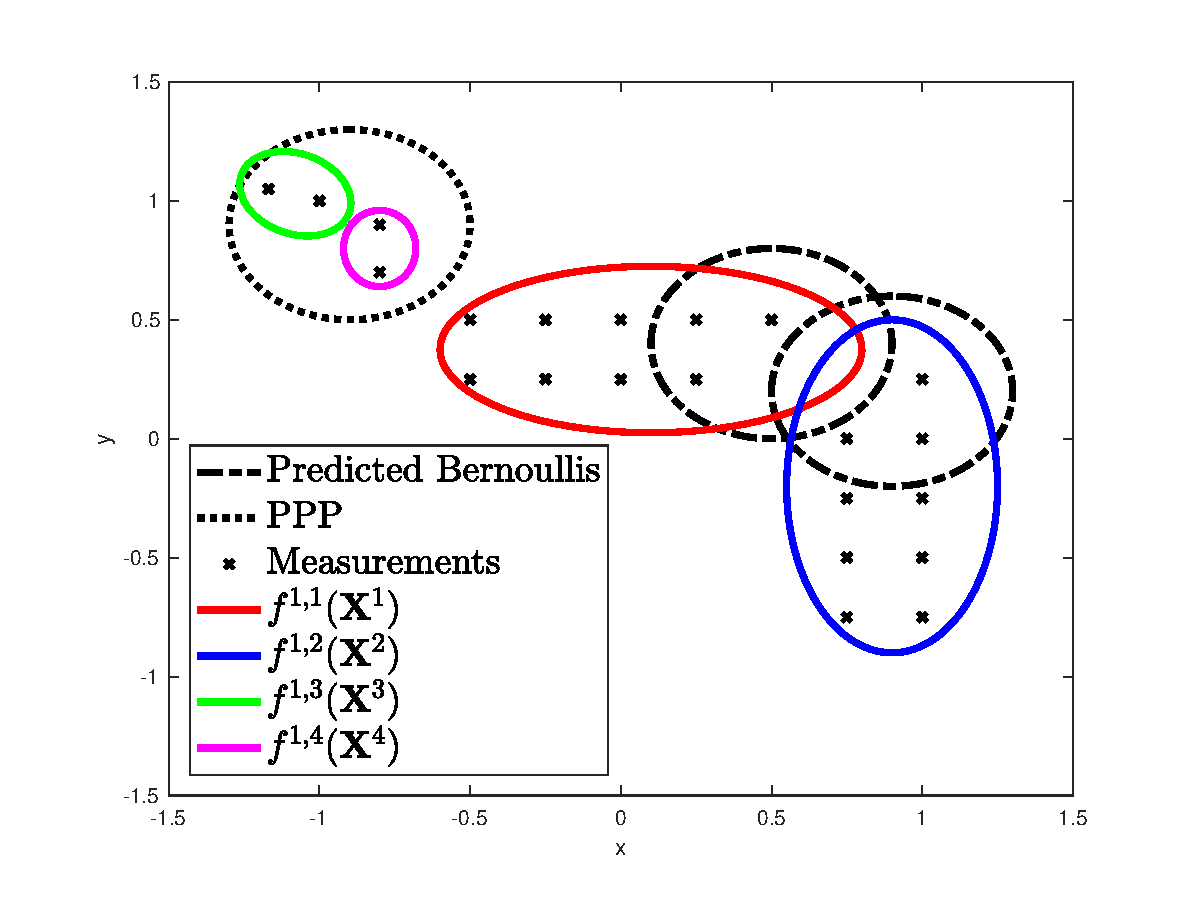
\includegraphics[width = 0.6\columnwidth]{example1.eps}
    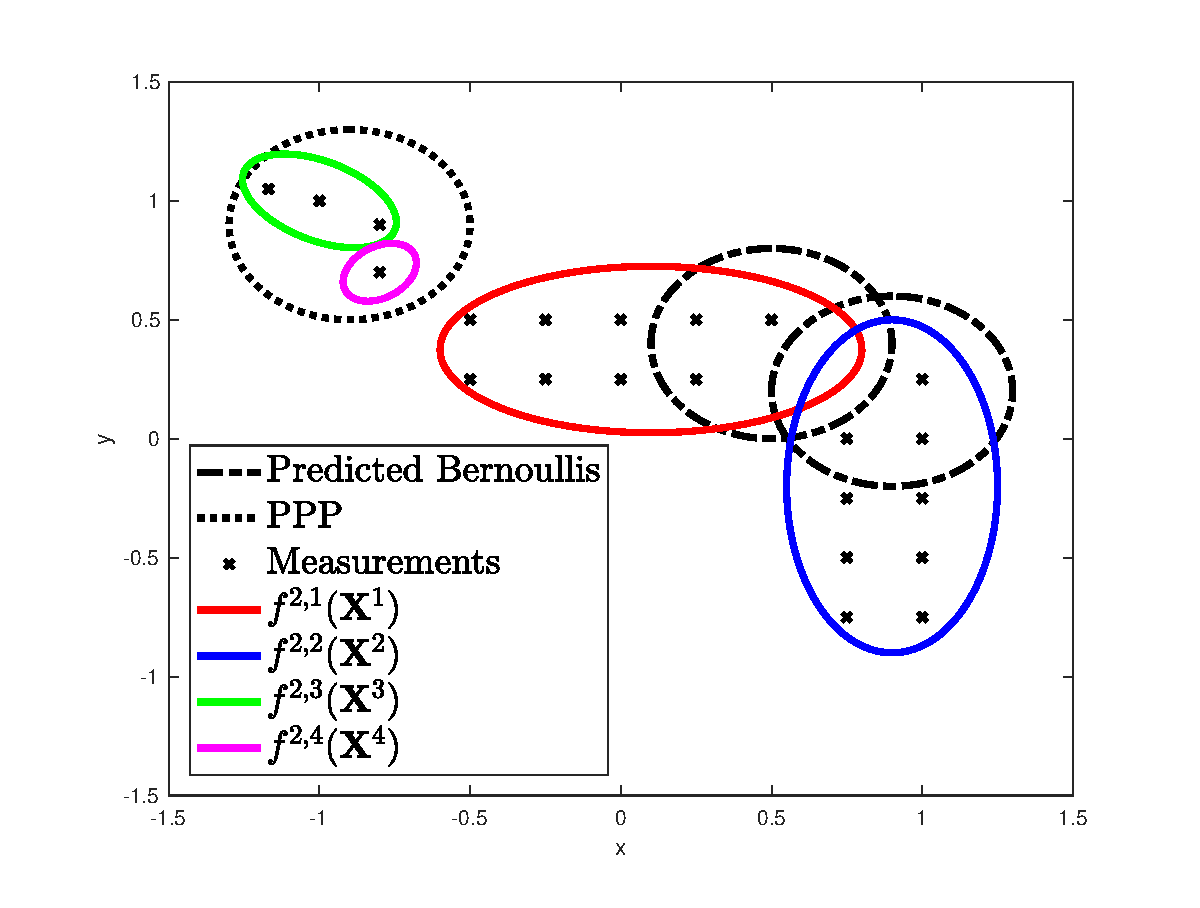
\includegraphics[width = 0.6\columnwidth]{example2.eps}
    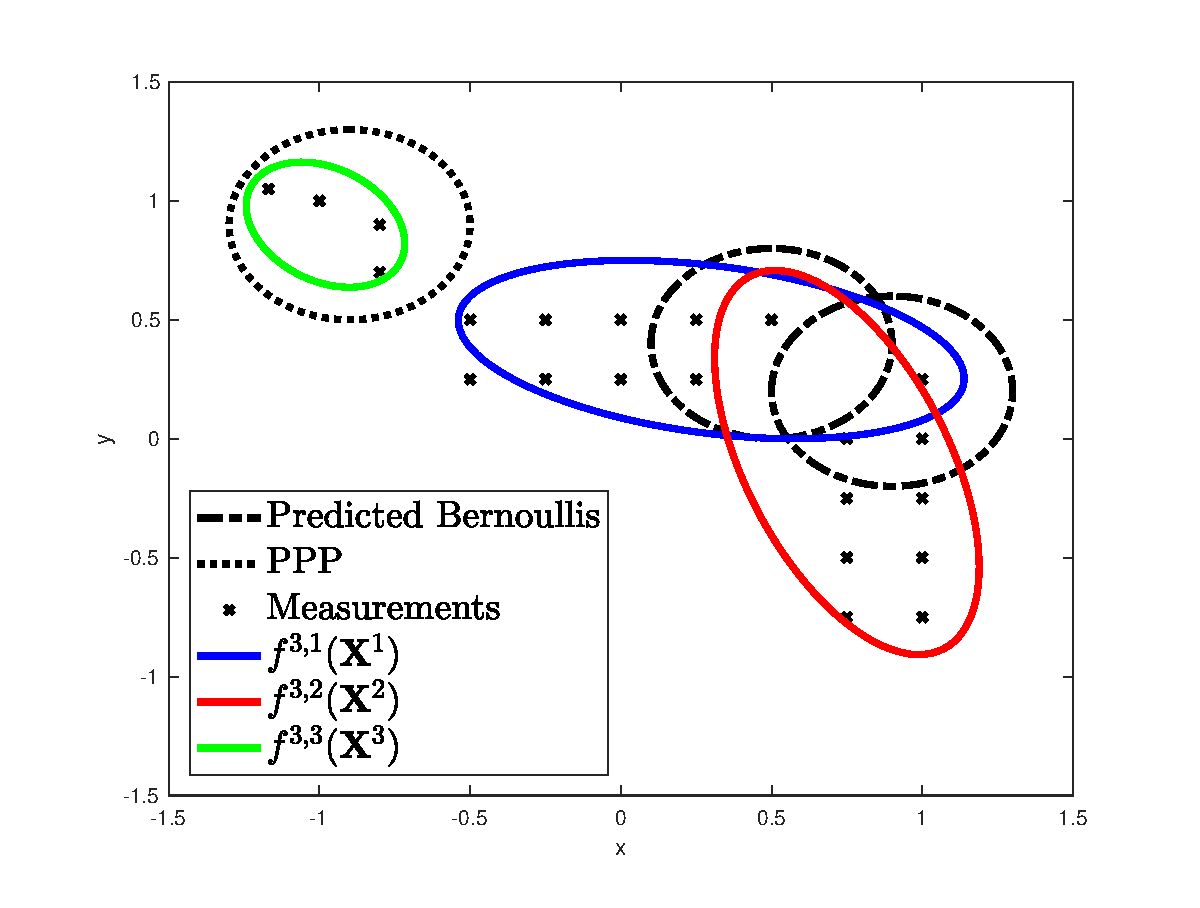
\includegraphics[width = 0.6\columnwidth]{example3.eps}
    \caption{Illustrative example with three MBs $f^1(\mathbf{X})$, $f^2(\mathbf{X})$ and $f^3(\mathbf{X})$ with weights $\mathcal{W}^1=0.4$, $\mathcal{W}^2=0.35$ and $\mathcal{W}^3=0.25$. Densities are presented by their level curves. Bernoullis marked in the same color \textcolor{red}{red}/\textcolor{blue}{blue} correspond to the measurement update of the same track. Bernoullis marked in \textcolor{red}{red} and \textcolor{blue}{blue} stand for the updates of previously detected targets, whereas Bernoullis marked in \textcolor{green}{green} and \textcolor{magenta}{magenta} stand for the first detections of undetected targets.}
    % \caption{Illustrative example with three MBs. $f^1(\mathbf{X})$ ($\mathcal{W}^1=0.4$) has four Bernoullis: $f^{1,1}(\mathbf{X}^1)$ and $f^{1,2}(\mathbf{X}^2)$ stand for the update of two detected targets, where as $f^{1,3}(\mathbf{X}^3)$ and $f^{1,4}(\mathbf{X}^4)$ stand for the detection of two potential new targets. $f^2(\mathbf{X})$ ($\mathcal{W}^2=0.35$) has four Bernoullis: $f^{2,1}(\mathbf{X}^1)$ and $f^{2,2}(\mathbf{X}^2)$ stand for the update of two detected targets, whereas $f^{2,3}(\mathbf{X}^3)$ and $f^{2,4}(\mathbf{X}^4)$ stand for the detection of two potential new targets. $f^3(\mathbf{X})$ ($\mathcal{W}^3=0.25$) has three Bernoullis: $f^{3,1}(\mathbf{X}^1)$ and $f^{3,2}(\mathbf{X}^2)$ stand for the update of two detected targets, whereas $f^{3,3}(\mathbf{X}^3)$ stands for the detection of a potential new target. Bernoullis marked with the same color correspond to the measurement update of the same (potential new) target.}
    \label{fig:example}
\end{figure*}

There are three major challenges related to this MB approximation. The first challenge is to determine the number of Bernoullis $|\hat{\mathbb{I}}|$ in the approximated MB, since different MB $f^j(\mathbf{X})$ may not all contain the same number of Bernoullis $|\mathbb{I}^j|$. Given $|\mathbb{M}|$ measurements, there are $2^{|\mathbb{M}|}-1$ possible ways in which we can form a subset of measurements. Each such subset can, in an association, be associated to a newly detected target. As a result, different global hypotheses may contain a different number of new tracks. Therefore, determining how many new tracks should be formed in the extended target PMB filter is a challenge. 

In this work, we choose to approximate the MBM as a single MB by merging. Then, the second challenge is to determine, for each $\iota \in \hat{\mathbb{I}}$, which Bernoullis $f^{j,i}(\mathbf{X})$ should be used to form $\hat{r}^{\iota}$ and $g^{\iota}(\mathbf{x})$. The Bernoullis in each MB are unordered\footnote{Note that the indexing of Bernoullis in each MB is merely used for notational convenience.} so determining how to select Bernoullis to merge across different MBs is a challenge\footnote{In this work, we choose not to merge Bernoullis within the same MB. An MB corresponds to a collection of independent potential targets. It is generally inappropriate to represent two or more independent targets with a single Bernoulli.}. Alternative solutions to address the first and the second challenges are discussed in Section V and VI.

% Once we have decided the number of Bernoullis $|\hat{\mathbb{I}}|$ in the approximated MB, and the selection of Bernoullis from the MBM to merge for each approximated Bernoulli $g^{\iota}(\mathbf{X}^{\iota})$, 
The last challenge is to determine how to merge the selected Bernoullis into a single Bernoulli. Compared to the first two challenges, the third challenge is relatively less difficult, e.g., given a Bernoulli mixture, one can simply take the weighted sum of different parameters. In extended target tracking, the merging of different target state densities is typically addressed by analytically minimizing the KL divergence \cite{phdextended,gammareduction}. In Section VII, we will discuss some implementation details regarding the merging of different Bernoullis under a common extended target model, called gamma Gaussian inverse Wishart (GGIW) \cite{phdextended,cphdextended}. 

We illustrate these three major challenges with the following example. 
\newtheorem{example}{Example}[section]
\begin{example}
\emph{Consider a two-dimensional scenario shown in Fig. \ref{fig:example}, with an MBM that contains three global hypotheses. For simplicity, we assume that each Bernoulli has existence probability equal to one. In this scenario, two detected targets are closely spaced, and it is ambiguous whether there are two closely spaced new targets or one bigger new target.}

\emph{It is simple to decide the number of pre-existing tracks, which is two in this case. The first challenge is determining how to choose the number of Bernoullis in the approximated MB. Because the new tracks in the three global hypotheses are all different, it is nontrivial to decide the exact number of tracks we should form in the approximated density.}

\emph{The second challenge is determining how to select the Bernoulli components to be merged. Given three global hypotheses, each of which has two pre-existing tracks, there are eight different ways in total to obtain the approximated MB representing detected targets. The problem becomes more complicated when we consider the approximation of new tracks, since the number of approximated Bernoullis representing newly detected targets is yet to be decided.}

\emph{The third challenge is determining how to merge the selected Bernoullis. For example, if we choose to merge $f^{1,1}(\mathbf{X}^1)$, $f^{2,1}(\mathbf{X}^1)$ and $f^{3,1}(\mathbf{X}^1)$, then we should seek for accurate merging techniques so that the approximated Bernoulli can retain as much information as possible from these three Bernoullis.}
\\\IEEEQEDopen
\end{example}

\subsection{Recycling}
For the approximated MB $g(\mathbf{X})$ with parameters (\ref{eq:approxmb}), the recycling method of \cite{recycle} can be applied to Bernoullis with low existence probability $\hat{r}^{\iota}$. The recycled components are approximated as being Poisson and are incorporated into the PPP representing undetected targets for generating possible new targets in subsequent steps. 
% The benefits of recycling in the point target PMBM and PMB filters have been demonstrated in \cite{performanceevaluation}.
% Suppose that a Bernoulli $g^{\iota}(\mathbf{X}^{\iota}), \iota\in\hat{\mathbb{I}}$, in the form of (\ref{eq:bernoulli}), is approximated by a PPP
% \begin{equation}
% \hat{g}^{\iota}(\mathbf{X}^{\iota}) = e^{-\mu}\prod_{\mathbf{x}\in \mathbf{X}}D(\mathbf{x}).
% \end{equation}
% As shown in \cite[p. 359]{rfs}, it is optimal to set $D(\mathbf{x})=\mu g^{\iota}(\mathbf{x})$, where $\mu=\hat{r}^{\iota}$. 
% % \begin{subequations}
% % \begin{align}
% %     D(\mathbf{x}) &= \mu f(\mathbf{x}),\\
% %     \mu &= r.
% % \end{align}
% % \end{subequations}
% The value of the KL divergence at this optimal choice is given by
% \begin{equation}
%     D_{\text{KL}}(g^{\iota}(\mathbf{X}^{\iota})||\hat{g}^{\iota}(\mathbf{X}^{\iota})) = \hat{r}^{\iota} + (1-\hat{r}^{\iota})\log(1-\hat{r}^{\iota}),
% \end{equation}
% and it is very small for existence probability $\hat{r}^{\iota}$ less than 0.1 \cite{recycle}. 
After recycling, the total PPP intensity of the set of undetected targets can be expressed as
\begin{equation}
    \hat{D}^u(\mathbf{x}) = D^u(\mathbf{x}) + \sum_{\iota\in\hat{\mathbb{I}}:\hat{r}^{\iota}<\tau}\hat{r}^{\iota}\hat{g}^{\iota}(\mathbf{x}),
\end{equation}
where $\tau$ is a threshold, and a typical choice is $\tau=0.1$.

The benefits of recycling in the point target PMBM and PMB filters have been discussed in \cite{recycle,performanceevaluation}. In this work, we utilize MB approximation methods and recycling to approximate the PMBM posterior density as a PMB.



% Given a measurement partitioning, a new track is created for each possible measurement cell. If the measurement cell is associated to a pre-existing track in the global hypothesis that corresponds to the particular data association, the new track that corresponds to this measurement cell would have zero existence probability. Given $|\mathbb{M}|$ measurements, there are $2^{|\mathbb{M}|}-1$ possible ways in which we can form a subset of measurements. Each such subset can, in an association, be associated to a potential new target. 

% A considerable difficulty in the development of the MBM merging algorithm is to approximate the MBM, in which each MB may contain different number of Bernoulli components $|\mathbb{I}^j|$, to a single MB. Main challenges include how many tracks $|\hat{\mathbb{I}}|$ should be created and how tracks should be formed. When forming a track, we should also consider the selection of the Bernoulli components to merge and the way to merge them. In Section IV and V, we discuss different alternative solutions to solve these problems.




% Note that the number of Bernoulli components in the approximated MB, i.e., $|\hat{\mathbb{I}}|$ is a variable which needs to be estimated, since it is unknown that how many measurement cells are formed in each possible data association. This is a remarkable difference between the extended target PMB filter and the point target PMB filter. In the latter case, each measurement creates a new track, so that the number of Bernoulli components in the approximated MB satisfies
% \begin{equation}
%     |\hat{\mathbb{I}}| = |\mathbb{I}^j| = |\mathbb{I}|+|\mathbb{M}|~\forall~j\in\mathbb{J}.
% \end{equation}

% In the point target PMBM filter, each measurement creates a new track, such that each updated MB has equal number of Bernoulli components, though each updated MB may contain different number of Bernoulli components with valid target existence probability due to the unknown number of targets that are detected for the first time.



% In this work, the MBM approximations for pre-existing tracks and new tracks are considered separately. 
\section{Track-oriented PMB Filter}
% The PMB form is an approximation to the full posterior representation (\ref{eq:pmbm}). Our objective is to approximate an MBM density $f(\mathbf{X})$, in which different MB density $f^j(\mathbf{X})$ may contain a different number of Bernoulli components, with a single MB. 
In this section, we seek to develop a well performing PMB filter by adapting the merging technique used in the point target TOMB/P filter \cite{pmbmpoint} to extended targets. We call the proposed filter track-oriented PMB (TO-PMB). Following a similar track-oriented merging approach \cite{pmbmpoint}, in the TO-PMB filter, single target hypotheses updating different tracks are assumed to be independent, and hypotheses comprising the same track are merged into a single Bernoulli across different global hypotheses. In what follows, we discuss the extended target TO-PMB filter, its connection to the LMB filter and the drawback of this track-oriented merging approach. 


% In this section, we start by exploring the possibility of adapting the two merging techniques used in the point target marginal MB filters \cite{pmbmpoint} to extended target filtering. Theoretically, it is possible to design a measurement cluster oriented PMB filter for extended target, analogous to the MOMB/P filter. The idea is to create a track for each measurement cell collecting all single target hypotheses updated by the measurement cell, and a track for each prior track containing only the missed detection hypothesis. However, a large number of tracks would be created following this approach due to the enormous number of ways to form measurement cluster, and different tracks may suffer from a seriously compatible problem. Thus, the measurement cluster oriented PMB filter for extended target is practically inadvisable. 

% Another strategy, which is analogous to the TOMB/P filter, is to create a track collecting all single target hypotheses updating the same target (existing or potential). In what follows, we discuss the so-called extended target TO-PMB filter, its connection to the LMB filter and the drawback of this track-oriented merging approach.

\subsection{Track formation}
Let us discuss the formations of new tracks and pre-existing tracks separately. For pre-existing tracks ($\iota\in\hat{\mathbb{I}}\cap\mathbb{I}$), the approximated Bernoulli is simply formed by merging all Bernoullis that correspond to the same track in global hypotheses:
\begin{equation}
    g^{\iota}(\mathbf{X}^{\iota}) \propto \sum_{j\in\mathbb{J}}\mathcal{W}^jf^{j,\mathfrak{L}(\iota)}(\mathbf{X}^{\mathfrak{L}(\iota)}), \iota\in\hat{\mathbb{I}}\cap\mathbb{I},
    \label{eq:tomerge}
\end{equation}
where $\mathfrak{L}(\iota)=i$ is a bijection that maps the index $i\in\mathbb{I}^j\cap\mathbb{I}$ to the index $\iota\in\hat{\mathbb{I}}\cap\mathbb{I}$; $f^{j,i}(\mathbf{X}^i)$ has existence probability and existence-conditioned PDF in the form of (\ref{eq:missUpdate}) or (\ref{eq:measUpdate}); $g^{\iota}(\mathbf{X}^{\iota})$ is in the form of (\ref{eq:approximatedBernoulli}); the proportionality denotes that normalization is required to ensure that the weights of different $f^{j,i}(\mathbf{x})$, i.e., $\mathcal{W}^jr^{j,i}$, sum to one (e.g., see \cite{ArdeshiriGOO:2015}).
% \footnote{The same also holds for (\ref{eq:tonew}), (\ref{eq:mstepjason}), (\ref{eq:mstepop}) and (\ref{eq:approxnewtrack}).}

The number of new tracks is determined by the number of different measurement cells associated to the background in different global hypotheses. Let $\mathcal{C}$ denote the set of measurement cells $\mathbf{C}$ that are associated to a newly detected target in any of the global hypotheses $\mathbb{J}$, and let $f^{\mathbf{C}}(\cdot)$ denote the corresponding Bernoulli density, see (\ref{eq:newUpdate}). In the TO-PMB filter, each measurement cell $\mathbf{C}\in\mathcal{C}$ results in a unique Bernoulli in the approximated MB $g(\mathbf{X})$, thus the number of new tracks formed in the TO-PMB filter is the number of cells in $\mathcal{C}$, i.e., $|\hat{\mathbb{I}}\setminus\mathbb{I}|=|\mathcal{C}|$. 
% Let $\mathbb{P}$ denote the set of all the possible non-empty subsets of measurement indices set $\mathbb{M}$, and let $\mathbf{C}_P$ denote the measurement cell formed by measurements with indices $P\in\mathbb{P}$. We assume that the subsets $P$ are indexed from 1 to $|\mathbb{P}|$, and the $\rho$th element is denoted as $P^{\rho}$. Further, if measurement cell $\mathbf{C}_{P^{\rho}}$ is hypothesised to be the detection of a potential new target, let $f^{\mathbf{C}_{P^{\rho}}}(\cdot)$ denote the Bernoulli density of the corresponding single target hypothesis. 
Further, we define a bijection $\mathfrak{F}(\iota)=\mathbf{C}$ that maps the index of a new track $\iota\in\hat{\mathbb{I}}\setminus\mathbb{I}$ to the measurement cell $\mathbf{C}\in\mathcal{C}$. For new tracks ($\iota\in\hat{\mathbb{I}}\setminus\mathbb{I}$), the approximated Bernoulli is formed by merging single target hypotheses updated by the same measurement cell across different global hypotheses, according to
\begin{equation}
    g^{\iota}(\mathbf{X}^{\iota}) \propto \sum_{j\in\mathbb{J}}\mathcal{W}^jf^{\mathfrak{F}(\iota)}(\mathbf{X})\Delta_{\mathfrak{F}(\iota)\in\mathcal{P}^j}, \iota\in\hat{\mathbb{I}}\setminus\mathbb{I},
    \label{eq:tonew}
\end{equation}
where $\mathcal{P}^j$ denotes the partition of measurements assigned to potential new targets in the $j$th global hypothesis, and $\Delta_{\mathbf{C}\in\mathcal{P}^j}$ is an indicator function, which is equal to one if and only if measurement cell $\mathbf{C}$ belongs to measurement partition $\mathcal{P}^j$.

\subsection{Connection to the LMB filter}
For filters based on a labelled MB conjugate prior, namely, the $\delta$-GLMB filter and its approximation the LMB filter, labels are augmented to target states to maintain tracks. It has been shown in \cite{pmbmpoint2} that the $\delta$-GLMB density is analogous to a type of MBM on a labelled state space, and that labels are not required for the conjugacy property of the MBM. In the LMB approximation, Bernoullis with the same label are merged across different MBs \cite{lmb}, while in the TO-PMB filter, Bernoullis updating the same track are merged. In general, it can be concluded that approximating the $\delta$-GLMB density with a LMB relies on a similar type of approximation as is used to approximate the PMBM density with a TO-PMB. 

% While the TO-PMB filter considers the unlabelled case, the track continuity can be made explicit by incorporating a label into the underlying state space \cite{pmbmpoint}.

\subsection{Drawback}
The track-oriented merging approach is simple to implement; nevertheless, it has several drawbacks. In the LMB filter and the TO-PMB filter, tracks are approximated as independent. This assumption holds well for the case that targets are well separated, however, the dependency between targets becomes inescapable when targets are closely spaced. Both the LMB filter and the TO-PMB filter suffer from large estimation errors when coalescence happens, see \cite{performanceevaluation} and \cite{pmbmpoint} respectively, for their performance evaluation on point target filtering. 

In addition to the above drawback, the track-oriented merging approach is particularly unfit for the extended target PMB filter, in which new tracks created by different measurement cells are approximated as independent. If some of the measurement cells have shared measurements, which is the typical case, the new tracks are highly dependent since they never co-exist in the same data association hypothesis, and approximating such tracks as independent may yield large errors. Also, creating as many new tracks as there are measurement cells often yields intractably many Bernoullis (tracks) with low existence probabilities. In Section VI, we will investigate techniques that are more accurate and yield much fewer tracks, thus mitigating all of these weaknesses simultaneously.

\section{Variational Multi-Bernoulli Filter}

As discussed in last section, approximating the MBM by the track-oriented merging approach is likely to yield large estimation errors. The key issue of this problem lies in approximating highly dependent new tracks as independent, which means that a more appropriate method should be used in approximating new tracks. In this section, we divide the MB approximation into two separate parts: one for the formation of new tracks and the other for the formation of pre-existing tracks. The premise of this implementation is that the pre-existing tracks and new tracks are assumed to be independent. Although there are situations where this approximation is less accurate, it is essential to our approach to obtain a tractable solution. 

Our goal is to approximate, in the minimum KL divergence sense, the posterior MBM with an MB that has two parts, corresponding to pre-existing and new tracks, respectively. As stated in Section \ref{section:kldecomposition}, this problem can be approximately solved by minimizing the KL divergences between the marginal density of the pre-existing/new tracks and its approximate MB density. Analytically minimizing such KL divergences is, however, still intractable; thus, we instead look for approximate solutions. 
For approximating the pre-existing tracks $\iota\in\hat{\mathbb{I}}\cap\mathbb{I}$, we employ the variational approximation technique in \cite{variational}, which can successfully address the potential coalescence problem suffered by the TO-PMB filter. Two variants of the variational MB algorithm are studied. We first review the variational MB algorithm implemented in \cite{variational}, then we study an alternative implementation of this algorithm that is inspired by the SJPDA filter \cite{sjpda}. For approximating the new tracks $\iota\in\hat{\mathbb{I}}\setminus\mathbb{I}$, we propose a greedy method to merge similar Bernoullis (tracks), in the sense of minimizing the KL divergence. 

% Theoretically, it is possible to apply the variational MB algorithm to the entire MBM by assuming that new tracks that correspond to different measurement cells are independent. As discussed in Section V, this assumption may yield large estimation error. Thus, it is problematic to incorporate the formation of new tracks into the variational MB algorithm for extended target filtering. 

% In the remaining part of this section, we omit the time index $k$ and drop the superscript of target set density, used to denote the detected targets, for the sake of notational clarity.


% \subsection{Approximate solution}
% Let $\mathbf{X}^o_k$ denote the set of targets that are detected before time step $k$, and let $\mathbf{X}^n_k$ denote the set of newly detected targets. It holds that the set of detected targets $\mathbf{X}^d_k$ is a disjoint union of $\mathbf{X}^o_k$ and $\mathbf{X}^n_k$, i.e., $\mathbf{X}^d_k=\mathbf{X}^o_k\uplus\mathbf{X}^n_k$. Given a global hypothesis $j\in\mathbb{J}$, the MB set density can be expressed as
% \begin{equation}
%     f^j_{k|k}(\mathbf{X}^d_k) = \sum_{\mathbf{X}^d_k=\mathbf{X}^o_k\uplus\mathbf{X}^n_k}f^{j,o}_{k|k}(\mathbf{X}^o_k)f^{j,n}_{k|k}(\mathbf{X}^n_k), \forall j\in\mathbb{J},
%     \label{eq:independentfact}
% \end{equation}
% where $f^{j,o}_{k|k}(\mathbf{X}^0_k)$ and $f^{j,n}_{k|k}(\mathbf{X}^n_k)$ are, respectively, MB densities with parameters
% \begin{subequations}
% \begin{align}
%     &\{r^{j,i},f^{j,i}(\cdot)\}_{i\in\mathbb{I}^j\cap\mathbb{I}},\\
%     &\{r^{j,i},f^{j,i}(\cdot)\}_{i\in\mathbb{I}^j\setminus\mathbb{I}}.
% \end{align}
% \end{subequations}
% We wish to approximate, in the minimum KL divergence sense, the posterior MBM with an MB that has two parts, corresponding to pre-existing and new tracks, respectively. 

% \newtheorem{problem}{Problem}[section]
% \newtheorem{theorem}{Theorem}[section]
% \begin{problem}
% \label{problem1}
% \emph{Find the MB $g_{k|k}(\mathbf{X}_k^d)$ that minimizes the KL divergence}
% \begin{equation}
%     D_{\text{KL}}(f_{k|k}(\mathbf{X}_k^d)||g_{k|k}(\mathbf{X}_k^d)),
%     \label{eq:joingMBkl}
% \end{equation}
% % \\=\underset{g}{\arg\min}-\int f_{k|k}(\mathbf{X}_k^d)\log g_{k|k}(\mathbf{X}_k^d)
% \emph{where $f_{k|k}(\mathbf{X}_k^d)$ is an MBM}
% \begin{equation}
%     f_{k|k}(\mathbf{X}_k^d) = \sum_{j\in\mathbb{J}}\mathcal{W}^j\sum_{\mathbf{X}^d_k=\mathbf{X}^o_k\uplus\mathbf{X}^n_k}f^{j,o}_{k|k}(\mathbf{X}^o_k)f^{j,n}_{k|k}(\mathbf{X}^n_k),
% \end{equation}
% \emph{and $g_{k|k}(\mathbf{X}_k^d)$ is the union of two independent MBs $g^o_{k|k}(\hat{\mathbf{X}}^o_k)$ and $g^n_{k|k}(\hat{\mathbf{X}}^n_k)$}
% \begin{equation}
%     g_{k|k}(\mathbf{X}_k^d) = \sum_{\mathbf{X}^d_k=\hat{\mathbf{X}}^o_k\uplus\hat{\mathbf{X}}^n_k}g^o_{k|k}(\hat{\mathbf{X}}^o_k)g^n_{k|k}(\hat{\mathbf{X}}^n_k),
% \end{equation}
% \end{problem}
% \emph{with parameters}
% \begin{subequations}
% \begin{align}
%     &\{\hat{r}^{\iota},g^{\iota}(\cdot)\}_{{\iota}\in\hat{\mathbb{I}}\cap\mathbb{I}},\\
%     &\{\hat{r}^{\iota},g^{\iota}(\cdot)\}_{{\iota}\in\hat{\mathbb{I}}\setminus\mathbb{I}}.
% \end{align}
% \end{subequations}

% As stated in Section \ref{section:kldecomposition}, Problem \ref{problem1} can be approximately solved by minimizing the KL divergences between the marginal density of the pre-existing/new tracks and its approximate MB density. Analytically minimizing such KL divergences is, however, still intractable; thus, we will instead look for approximate solutions.

% % We propose an approximate solution to Problem \ref{problem1} that is based on minimization of an upper bound of the true objective, following a similar process to \cite[Section III]{variational}.
% % \begin{theorem}
% % \label{theorem1}
% % The objective in Problem \ref{problem1} has an upper bound that, when minimizing over $g^o(\cdot)$ and $g^n(\cdot)$, allows for the KL divergence minimization (Problem \ref{problem1}) to be broken down into two separate KL divergence minimization problems:
% % \begin{multline}
% % \underset{g^o}{\arg\min}\int\sum_{j\in\mathbb{J}}\mathcal{W}^jf^{j,o}_{k|k}(\mathbf{X}^o_k)\log(g^o_{k|k}(\mathbf{X}^o_k))\delta\mathbf{X}^o\\+\underset{g^n}{\arg\min}\int\sum_{j\in\mathbb{J}}\mathcal{W}^jf^{j,n}_{k|k}(\mathbf{X}^n_k)\log(g^n_{k|k}(\mathbf{X}^n_k))\delta\mathbf{X}^n.
% % \end{multline}
% % \begin{subequations}\label{eq:subproblems}
% % \begin{align}
% %     & \underset{g^o}{\arg\min}~D\bigg( \sum_{j\in\mathbb{J}} \mathcal{W}_j f^{j,o}_{k|k} (\setX^o_k)) || g^o_{k|k}(\setX^o_k) \bigg), \label{eq:pre-existingtrackapprox} \\
% %     & \underset{g^n}{\arg\min}~D\bigg( \sum_{{j\in\mathbb{J}}} \mathcal{W}_j f^{j,n}_{k|k} (\setX^n_k) || g_{k|k}^n(\setX^n_k)  \bigg).
% %     \label{eq:newtrackapprox}
% % \end{align}
% % \end{subequations}
% % \hfill$\square$
% % \end{theorem}

% % The proof of Theorem \ref{theorem1} is given in Appendix \ref{appendix:proof}. Theorem \ref{theorem1} shows that an approximate solution of Problem \ref{problem1} can be obtained by finding the best-fitting MB approximations that satisfy
% % \begin{subequations}
% % \begin{align}
% %     g^o_{k|k}(\mathbf{X}^o_k) &=  \sum_{j\in\mathbb{J}}\mathcal{W}^jf^{j,o}_{k|k}(\mathbf{X}^o_k),\\
% %     g^n_{k|k}(\mathbf{X}^n_k) &= \sum_{j\in\mathbb{J}}\mathcal{W}^jf^{j,n}_{k|k}(\mathbf{X}^{n}_k).
% % \end{align}
% % \end{subequations}
% % The proof of Theorem \ref{theorem1} is given in Appendix \ref{appendix:proof}. Analytically minimizing the KL divergences (\ref{eq:subproblems}) is, however, still intractable; thus, we will instead look for approximate solutions.


% % In order to approximate the pre-existing and new tracks separately, our first task is to derive the marginalized MBM density $p^o_{k|k}(\mathbf{X}^o_k)$ for pre-existing tracks, where new tracks are marginalized out, and the marginalized MBM density $p^n_{k|k}(\mathbf{X}^n_k)$ for new tracks, where pre-existing tracks are marginalized out. Then, we need to find good MB approximations for $p^o_{k|k}(\mathbf{X}^o_k)$ and $p^n_{k|k}(\mathbf{X}^n_k)$. Assuming that the pre-existing and new tracks are independent, the MBM set density of detected targets can be approximated as
% % \begin{equation}
% % \begin{split}
% %     \sum_{j\in\mathbb{J}}\mathcal{W}^jf^j_{k|k}(\mathbf{X}^d_k) &\approx\sum_{\mathbf{X}^d_k=\mathbf{X}^o_k\uplus\mathbf{X}^n_k} p^o_{k|k}(\mathbf{X}^o_k)p^n_{k|k}(\mathbf{X}^n_k)\\
% %     &\approx\sum_{\mathbf{X}^d_k=\mathbf{X}^o_k\uplus\mathbf{X}^n_k}g^o_{k|k}(\mathbf{X}^o_k)g^n_{k|k}(\mathbf{X}^n_k)\\
% %     &\equiv g_{k|k}(\mathbf{X}^d_k),
% % \end{split}
% %     \label{eq:prenewindependent}
% % \end{equation}
% % where $g^o_{k|k}(\mathbf{X}^o_k)$ and $g^n_{k|k}(\mathbf{X}^n_k)$ are, respectively, MBs of approximated pre-existing and new tracks, and the marginal densities $p^o_{k|k}(\mathbf{X}^o_k)$ and $p^n_{k|k}(\mathbf{X}^n_k)$ can be obtained as
% % \begin{subequations}
% % \begin{align}
% %     p^o_{k|k}(\mathbf{X}^o_k) &=  \sum_{j\in\mathbb{J}}\mathcal{W}^jf^{j,o}_{k|k}(\mathbf{X}^o_k),\\
% %     p^n_{k|k}(\mathbf{X}^n_k) &= \sum_{j\in\mathbb{J}}\mathcal{W}^jf^{j,n}_{k|k}(\mathbf{X}^{n}_k).
% % \end{align}
% % \label{eq:marginalMBM}
% % \end{subequations}

% % However, analytically deriving $P(\mathbf{X}^e_k)$ and $P(\mathbf{X}^p_k)$ is intractable. To address this problem, we seek an approximate representation of $P(\mathbf{X}^e_k)$ and $P(\mathbf{X}^p_k)$ by assuming that the pre-existing and new tracks are independent. Under this assumption, we can easily obtain
% % \begin{subequations}
% % \begin{align}
% %     P(\mathbf{X}^e_k) &=  \sum_{j\in\mathbb{J}}\mathcal{W}^jf^j_{k|k}(\mathbf{X}^e_k),\\
% %     P(\mathbf{X}^p_k) &= \sum_{j\in\mathbb{J}}\mathcal{W}^jf^j_{k|k}(\mathbf{X}^p_k),
% % \end{align}
% % % \label{eq:prenewindependent}
% % \end{subequations}
% % and the MBM set density of detected targets can be expressed as
% % \begin{equation}
% % \begin{split}
% %     \sum_{j\in\mathbb{J}}\mathcal{W}^jf^j_{k|k}(\mathbf{X}^d_k) &=\sum_{\mathbf{X}^d_k=\mathbf{X}^e_k\uplus\mathbf{X}^p_k} P(\mathbf{X}^e_k)P(\mathbf{X}^p_k)\\&= \sum_{\mathbf{X}^d_k=\mathbf{X}^e_k\uplus\mathbf{X}^p_k}\sum_{j\in\mathbb{J}}\mathcal{W}^jf^j_{k|k}(\mathbf{X}^e_k)f^j_{k|k}(\mathbf{X}^p_k).
% %     \end{split}
% %     \label{eq:prenewindependent}
% % \end{equation}


% % Given an updated MBM, the Bernoullis describing the pre-existing tracks in $f^{j,o}_{k|k}(\mathbf{X}^o_k)$ and the Bernoullis describing the new tracks in $f^{j,n}_{k|k}(\mathbf{X}^n_k)$ can be separated by keeping track of the predicted index of each Bernoulli being updated. 
% For approximating the pre-existing tracks $\iota\in\hat{\mathbb{I}}\cap\mathbb{I}$, we employ the variational approximation technique in \cite{variational}, which can successfully address the potential coalescence problem suffered by the TO-PMB filter. Two variants of the variational MB algorithm are studied. We first review the variational MB algorithm implemented in \cite{variational}, then we study an alternative implementation of this algorithm that is inspired by the SJPDA filter \cite{sjpda}. For approximating the new tracks $\iota\in\hat{\mathbb{I}}\setminus\mathbb{I}$, we propose a greedy method to merge similar Bernoullis (tracks), in the sense of minimizing the KL divergence. In the remaining part of this section, we omit the time index $k$ and drop the superscript of target set density, used to denote previously or newly detected targets, for the sake of notation clarity.

% Recall that our goal is obtain an approximated MB that can retain as much information from the MBM as possible. A nature choice for solving this problem is to minimize the distortion between the MBM and the approximated MB.
% One such strategy, inspired by the work of the point target variational MB filter \cite{variational}, is to find the best-fitting MB that minimizes the KL divergence from the MBM of the PMBM posterior. More importantly, the potential coalescence problem suffered by the track-oriented PMB filter can be successfully addressed by the variational MB algorithm.

% In this section, we investigate the possibility of applying the variational MB algorithm to extended target filtering. We first review the variational MB algorithm implemented in \cite{variational}, then we study an alternative implementation of this algorithm that is inspired by the SJPDA filter \cite{sjpda}. After analyzing the limitations of directly adapting the two variants of the variational MB algorithm to extended target filtering, we present a method that considers separate approximation approaches for forming pre-existing and new tracks. This new merging approach can successfully mitigate the problems that we encounter in the development of an extended target PMB filter.




% The variational MB algorithm can be initialized with the marginal association probabilities (\ref{eq:marginalprob}). In the work of the point target PMB filter \cite{variational}, the data association problem is formulated as a maximization problem using a graphical model, and the estimates of marginal probabilities are obtained using loopy belief propagation \cite{lbp}.

% For the pre-existing tracks, the MBM is merged using the variational MB algorithm. In addition to the implementation used in \cite{variational}, we study an alternative implementation based on optimal assignment. 

\subsection{Pre-existing track formation}
Because the number of pre-existing tracks remains the same after updating, the variational MB algorithm, proposed in \cite{variational} for point target filtering\footnote{In the point target filtering, each measurement creates a new track, hence, different global hypotheses consist of the same number of tracks.}, can be easily applied to the pre-existing track approximation in the extended target PMB filter. 

In the variational MB algorithm, the goal is to obtain an approximate MB $g(\mathbf{X})$ that minimizes the KL divergence:
\begin{multline}
\underset{g}{\arg\min}~D_{\text{KL}}(f(\mathbf{X})||g(\mathbf{X})) \\= \underset{g}{\arg\min}-\int f(\mathbf{X})\log g(\mathbf{X})\delta\mathbf{X},
\label{eq:kl}
\end{multline}
where $f(\mathbf{X})$ is an MBM describing the pre-existing tracks, with parameters
\begin{equation}
    \{(\mathcal{W}^j,\{r^{j,i},f^{j,i}(\cdot)\}_{i\in\mathbb{I}^j\cap\mathbb{I}})\}_{j\in\mathbb{J}}.
\end{equation}
An approximate solution of (\ref{eq:kl}) is based on minimizing the upper bound of the true objective, following a similar process to expectation-maximization (EM) \cite{em}. In this approach, the correspondences between the Bernoullis in $f(\mathbf{X})$ and the Bernoullis in $g(\mathbf{X})$ are treated as missing data. 

By simplifying the MB set integral in (\ref{eq:kl}) into a series of Bernoulli integrals, and using the log-sum inequality, an approximate upper bound of the objective (\ref{eq:kl}) can be expressed as \cite{variational}
\begin{multline}
D_{\text{UB}}(f(\mathbf{X})||g(\mathbf{X}))= -\sum_{j\in\mathbb{J},\pi\in\Pi^j_N}\mathcal{W}^jq^j(\pi^j)\\\times\sum_{\iota\in\hat{\mathbb{I}}\cap\mathbb{I}}\int f^{j,\pi^j(\mathfrak{L}(\iota))}(\mathbf{X})\log g^{\iota}(\mathbf{X})\delta \mathbf{X},
\label{eq:vaorigin}
\end{multline}
where $N$ denotes the number of Bernoullis that correspond to pre-existing tracks in each MB of $f(\mathbf{X})$ and the approximated MB $g(\mathbf{X})$, i.e., $N=|\hat{\mathbb{I}}\cap\mathbb{I}|$; $\Pi^j_N$ is the set of all ways to assign the Bernoullis $f^{j,i}(\mathbf{X}^i), i\in\mathbb{I}^j\cap\mathbb{I}, j\in\mathbb{J}$ to the Bernoullis $g^{\iota}(\mathbf{X}^{\iota}), \iota\in\hat{\mathbb{I}}\cap\mathbb{I}$; the missing data $q^j(\pi^j)$ is constrained to vary only with the $j$th MB, and satisfies $q^j(\pi^j)\geq0$ and  $\sum_{\pi^j\in\Pi^j_N} q^j(\pi^j) = 1$. The standard method for optimizing (\ref{eq:vaorigin}) is block coordinate descent, which alternates between minimization with respect to $g^{\iota}(\mathbf{X}^{\iota})$ (M-step) and $q_j(\pi^j)$ (E-step) \cite{variational}.

Because solving the minimization problem (\ref{eq:vaorigin}) suffers from combinatorial complexity, approximation is needed to obtain a tractable solution. Here, two different approximation methods, and their limitations to extended target filtering, are studied.

\subsubsection{Efficient approximation of feasible set}

Because the minimization problem of (\ref{eq:vaorigin}) involves missing data $q^j(\pi^j)$ for every MB $f^j(\mathbf{X})$, a simplified missing data representation is desirable. The minimization of the upper bound (\ref{eq:vaorigin}) can be solved approximately as \cite{variational}
\begin{equation}
\operatornamewithlimits{argmin}_{q(h,\iota)\in\mathcal{M}}-\sum_{\iota\in\hat{\mathbb{I}}\cap\mathbb{I}}\int\bigg(\sum_{h\in\mathbb{H}}q(h,\iota)f^h(\mathbf{X})\bigg)\log g^{\iota}(\mathbf{X})\delta\mathbf{X},
\label{eq:feasibleset}
\end{equation}
where $\mathbb{H}$ is the index set of single target hypotheses included in the global hypotheses indexed by $j\in\mathbb{J}$, $q(h,\iota)$ is a simplified representation of $q^j(\pi^j)$, which specifies the weight of single target hypothesis density $f^h(\mathbf{X}^h)$\footnote{The same single target hypothesis may be included in different global hypotheses, thus it satisfies that $|\mathbb{H}|\leq\sum_{j\in\mathbb{J}}|\mathbb{I}^j|$. We use the single superscript $h$ to denote the index of single target hypothesis density in order to distinguish from the double superscript $\{j,i\}$, which denotes the indices of Bernoullis in the MBM.} in the new Bernoulli component $g^{\iota}(\mathbf{X}^{\iota})$, and the feasible set $\mathcal{M}$ is an approximation needed for tractability
\begin{multline}
    \mathcal{M} = \Bigg\{q(h,\iota)\geq0\Bigg|\sum_{h\in\mathcal{H}}q(h,\iota)=1 ~\forall~ \iota\in\hat{\mathbb{I}\cap\mathbb{I}},\\\sum_{\iota\in\hat{\mathbb{I}}\cap\mathbb{I}}q(h,\iota)=p_h ~\forall~ h\in\mathbb{H}\Bigg\}.
    \label{eq:polytope}
\end{multline}
The constraint $p_h$ satisfies $p_h=\sum_{\iota\in\hat{\mathbb{I}}\cap\mathbb{I}}p_{\iota}(h)$, where
\begin{equation}
    p_{\iota}(h)=
      \sum_{j\in\mathbb{J}}\mathcal{W}^j\Delta_{f^{j,\mathfrak{L}(\iota)}(\mathbf{X}^{\mathfrak{L}(\iota)})=f^h(\mathbf{X}^h)}, \iota\in\hat{\mathbb{I}}\cap\mathbb{I}
\label{eq:marginalprob}
\end{equation}
% \begin{subequations}
% \begin{align}
%     p_{\iota}(h) &= \sum_{j\in\mathbb{J}}\mathcal{W}^j\Delta_{f^{j,\iota}(\mathbf{X})=f^h(\mathbf{X})}, \iota\in\mathbb{I}\cap\mathbb{I}^j\\
%     p_{\iota}(h) &= \sum_{j\in\mathbb{J}}\mathcal{W}^j\Delta_{\mathbf{C}_{P^{\rho}}\in \mathcal{P}^j}, \iota\in\hat{\mathbb{I}}\setminus\mathbb{I},
% \end{align}
% \label{eq:marginalprob}
% \end{subequations}
Note that here the missing data distribution is no longer constrained to vary only with the global hypotheses. In this case, each approximated Bernoulli can be expressed as the weighted sum of different single target hypothesis densities, and the M-step becomes
\begin{equation}
g^{\iota}(\mathbf{X}^{\iota}) \propto \sum_{h\in\mathbb{H}}q(h,\iota)f^h(\mathbf{X}^h), \iota\in\hat{\mathbb{I}}\cap\mathbb{I},
\label{eq:mstepjason}
\end{equation}
while the E-step reverts to:
\begin{align}
\operatornamewithlimits{argmin}_{q(h,\iota)}\sum_{h\in\mathbb{H}}\sum_{\iota\in\hat{\mathbb{I}}\cap\mathbb{I}}&-q(h,\iota)\int f^h(\mathbf{X})\log g^{\iota}(\mathbf{X})\delta \mathbf{X},\label{eq:esteplp}\\
\text{subject to}&\sum_{\iota\in\hat{\mathbb{I}}\cap\mathbb{I}}q(h,\iota) = p_h~\forall~h,\notag\\
&\sum_{h\in\mathbb{H}}q(h,\iota) = 1~\forall~\iota,\notag\\
&q(h,\iota) \geq 0~\forall~h,\iota.\notag
\end{align}
% \begin{align*}
%     \text{subject to   } &\sum_{\iota\in\hat{\mathbb{I}}\cap\mathbb{I}}q(h,\iota) = p_h~\forall~h,\\
%     &\sum_{h\in\mathbb{H}}q(h,\iota) = 1~\forall~\iota,\\
%     &q(h,\iota) \geq 0~\forall~h,\iota.
% \end{align*}
Problem of this type can be solved using methods such as the simplex algorithm \cite{simplex}. 

The variational MB algorithm based on efficient approximation of feasible missing data set can be initialized with the marginal association probabilities (\ref{eq:marginalprob}). Although exact calculation of these quantities is intractable for a data association problem with combinatorial complexity, we can obtain approximated estimates by only considering truncated global hypotheses with non-negligible weights using data association approximation methods, such as \cite{pmbmextended2,soextended}.


% \subsection{Limitations to extended target filtering}
% The point target variational MB algorithm is initialized with marginal association probabilities that are approximated using loopy belief propagation (LBP) \cite{lbp}. Unfortunately, the graphical model formulated in \cite{lbp} is based on the assumption that each target may give rise to at most one measurement per time step. Thus, LBP is not suitable for approximating the marginal association probabilities for extended target filtering. An alternative method to calculate the marginal association probabilities is brute force. Although exact calculation of these quantities is intractable for a data association problem with combinatorial complexity, we can obtain approximated estimates by only considering truncated global hypotheses with non-negligible weights. 





\subsubsection{Most likely assignment}

The number of MBs in the MBM can be kept at a tractable level after truncating the global hypotheses with negligible weights. This allows us to study an alternative approach to solving the minimization problem of (\ref{eq:vaorigin}), following a similar approach to the Kullback-Leibler SJPDA (KLSJPDA) \cite{sjpda}. The KLSJPDA filter seeks to find the ordered distribution in the same unordered family, such that the new density can be most accurately approximated with a Gaussian density, in the KL sense. In the JPDA filter, the number of targets is assumed to be known, and the joint state of multiple targets are represented as a vector. As a comparison, given that each global hypothesis consists of the same number of pre-existing tracks, the multi-target RFS density will also have fixed cardinality. The similarities between the KLSJPDA filter and the variational MB filter were further explored in \cite{variational}.

Let us go back to the approximated upper bound (\ref{eq:vaorigin}) that we want to minimize. Suppose that Bernoullis in different MBs are indexed by the same superscript $i$ if they correspond to single target hypotheses updating the same track, and that only Bernoullis with the same superscript $i$ can be merged. Because the approximate MB density is invariant to the indexing of the Bernoullis it contains, the selection of the assignment mapping $\pi$ in each MB will not change the MBM $f(\mathbf{X})$, but only will determine which Bernoullis are going to be merged. The minimization problem can be interpreted as the Bernoullis in each MB are permuted in such a manner that the upper bound (\ref{eq:vaorigin}) is minimized but the density of the reordered $f(\mathbf{X})$ remains unchanged. 

Empirically, we found that finding a set of most likely assignments for each MB in the truncated MBM is computationally heavy. Hence, we choose to find the single most likely assignment $\hat{\pi}^j$ for each MB $f^j(\mathbf{X})$. In this case, the missing data distribution under each MB is a point mass, i.e.,  $q^{j}(\hat{\pi}^{j})=1$, and the the minimization of (\ref{eq:vaorigin}) with respect to the missing data distribution can be expressed as
\begin{equation}
    \hat{\pi}^j = \operatornamewithlimits{argmin}_{\pi^j}-\sum_{\iota\in\hat{\mathbb{I}}\cap\mathbb{I}}\int f^{j,\pi^j(\mathfrak{L}(\iota))}(\mathbf{X})\log g^{\iota}(\mathbf{X})\delta \mathbf{X}, j\in\mathbb{J},
    \label{eq:estepoptimal}
\end{equation}
where the most likely assignment $\hat{\pi}^j$ can be obtained using methods such as the auction algorithm \cite{auction}. The minimization of (\ref{eq:vaorigin}) with respect to the approximated MB $g(\mathbf{X})$ simplifies to 
\begin{equation}
    g^{\iota}(\mathbf{X}^{\iota}) \propto \sum_{j\in\mathbb{J}}\mathcal{W}^jf^{j,\hat{\pi}^j(\mathfrak{L}(\iota))}(\mathbf{X}^{\hat{\pi}^j(\mathfrak{L}(\iota))}), \iota\in\hat{\mathbb{I}\cap\mathbb{I}}.
\label{eq:mstepop}
\end{equation}
This means that each approximated Bernoulli in $g(\mathbf{X})$ can be obtained by merging Bernoullis in $f(\mathbf{X})$ with the same assignment mapping. 

% The premise of this variational MB algorithm using optimal assignment is based on the assumption that the number of Bernoullis in the approximated MB $g(\mathbf{X})$ is the same as the number of Bernoullis in each MB of the MBM $f(\mathbf{X})$. However, this does not hold for the MBM representing the multiple extended target set density, in which each MB may contain different number of Bernoullis. In practical implementation, dummy Bernoullis with zero existence probability can be appended to make the number of Bernoullis of each MB in the MBM in line with the approximated MB.
% Thus, it would be problematic to adapt such a variational MB algorithm to extended target filtering. 

% \subsubsection{Limitations}
% When applying the variational MB algorithm to extended target filtering, a few problems need to be carefully considered. First, tractability would be harmed, if we consider all the measurement cells that are associated to the new targets such that the size of the set of single target hypotheses can be very large. Second, the existence probability of approximated Bernoullis can be underestimated by assuming highly correlated new tracks to be independent. This is further illustrated in an example given in Section \ref{section:newtracks}. Thus, it would be problematic to incorporate the formation of new tracks into the variational MB algorithm for extended target filtering. 

% Let $A^j$ denote the data association for the $j$th updated hypothesis, and we assume that $A^j$ consists of index cells $C^j_i$, satisfying $\uplus_{i\in\mathbb{I}^j}C^j_i=\mathbb{M}\cup\mathbb{I}$. Further, let $N^j$ denote the number of non-empty measurement cell $\mathbf{C}_{C^j_i}$ given data association $A^j$. For $b\in\{1,...,N^j\}$, a single target hypothesis with Bernoulli density $f^{j,|\mathbb{I}|+b}(\mathbf{X}^{|\mathbb{I}|+b})$ is created for each non-empty measurement cell $\mathbf{C}_{C^j_i}$, which hypothesises the detection of a possible new born target. If a non-empty measurement cell is associated to a pre-existing track, then existence probability would be zero in the corresponding single target hypothesis. A consequence
% of this is that many of the Bernoulli components $f^{j,i}(\mathbf{X}^i)$
% have zero existence probability.




% In this subsection, the MBM describing new tracks is disregarded, and we denote the MBM $f(\mathbf{X})$ describing pre-existing tracks as $\{(\mathcal{W}^j,\{r^{j,i},f^{j,i}(\cdot)\}_{i=1}^N\}_{j\in\mathbb{J}}$,
% % \begin{equation}
% % \{(\mathcal{W}^j,\{r^{j,i},f^{j,i}(\cdot)\}_{i=1}^N\}_{j\in\mathbb{J}},
% % \end{equation}
% where $N$ is the number of pre-existing tracks. A variational method was presented in \cite{variational} to obtain the best-fitting MB $g(\mathbf{X})$ that minimises the set KL divergence from the MBM distribution $f(\mathbf{X})$:
% \begin{equation}
% \underset{g}{\arg\min}\int f(\mathbf{X})\log\frac{f(\mathbf{X})}{g(\mathbf{X})} = \underset{g}{\arg\max}\int f(\mathbf{X})\log g(\mathbf{X})d\mathbf{X}.
% \label{eq:kl}
% \end{equation}
% An approximate solution is based on minimising the upper bound of the true objective (\ref{eq:kl}), following a similar process to expectation-maximisation \cite{em}. The correspondence between the underlying Bernoulli distribution in $f(\mathbf{X})$ and the Bernoulli component in the best-fitting distribution $g(\mathbf{X})$ is treated as missing data $q(\pi)$. An approximated upper bound to the objective of (\ref{eq:kl}) is given by \cite{variational}
% \begin{multline}
% D_{\text{UB}}(f(\mathbf{X})||g(\mathbf{X}))= -\sum_{j\in\mathbb{J},\pi\in\Pi^j_N}\mathcal{W}^jq_j(\pi^j)\\\times\sum_{i=1}^N\int f^{j,\pi^j(i)}(\mathbf{X})\log g^{i}(\mathbf{X})\delta \mathbf{X},
% \label{eq:vaorigin}
% \end{multline}
% \begin{multline}
% D_{\text{UB}}(f(\mathbf{X})||g(\mathbf{X}))= -T\cdot\sum_{j\in\mathbb{J},\pi\in\Pi_N}\mathcal{W}^jq_j(\pi)\log q_j(\pi)\\-\sum_{j\in\mathbb{J},\pi\in\Pi_N}\mathcal{W}^jq_j(\pi)\sum_{i=1}^N\int f^{j,\pi(i)}(\mathbf{X})\log g^{i}(\mathbf{X})\delta \mathbf{X},
% \label{eq:vaorigin}
% \end{multline}
% where $\Pi_N$ is the set of all ways to assign the Bernoulli components in the $j$th MB $f^j(\mathbf{X})$ to the Bernoulli components in $g(\mathbf{X})$. 
% where $\Pi^j_N$ is the set of all ways to assign the Bernoulli components in the $j$th MB $f^j(\mathbf{X})$ to the Bernoulli components in $g(\mathbf{X})$; the missing data $q_j(\pi^j)$ is constrained to vary only with the $j$th MB, and it satisfies $q_j(\pi^j)\geq0$ and  $\sum_{\pi^j\in\Pi^j_N} q_j(\pi^j) = 1$. The standard method for solving the form of (\ref{eq:vaorigin}) is by block coordinate descent, which alternates between minimisation with respect to $g^i(\mathbf{X})$ (M-step) and $q_j(\pi^j)$ (E-step) \cite{variational}.

% These two steps can be solved as:
% \begin{equation}
%     g^{i}(\mathbf{X}) = \sum_{j\in\mathbb{J},\pi\in\Pi_N}\mathcal{W}^jq_j(\pi)f^{j,\pi(i)}(\mathbf{X})),
%     \label{eq:mstep}
% \end{equation}
% \begin{equation}
%     q_j(\pi)\propto \prod_{i=1}^N\exp\bigg(\frac{
%     1}{T}\int f^{j,\pi(i)}(\mathbf{X})\log g^{i}(\mathbf{X})\delta \mathbf{X}\bigg).
%     \label{eq:estep}
% \end{equation}
% \subsection{Separate pre-existing and new track formation}

% In the update step of the PMB filter, single target hypotheses representing newly detected targets are formed by updating the same PPP with different measurement cells, while single target hypotheses representing already detected targets are formed by updating independent Bernoulli components with different measurement cells. Considering from this aspect, the dependency between different new tracks that are created by similar measurement cells could be significantly stronger than the dependency between different pre-existing tracks that are updated by the same group of measurement cells. 

% In the extended target PMBM filter, different global hypotheses may contain different number of new tracks, thus making the variational MB approximation difficult to implement. In this work, we choose to divide the MBM approximation into two separate parts: one for the formation of new tracks and the other for the formation of pre-existing tracks. The premise of this implementation is that we assume that the pre-existing tracks and new tracks are independent. Although this independence assumption is likely to become worse when two similar measurement cells, in two associations, are associated to a detected target and a new target that are in close distance respectively, it is essential for tractability. 


% \subsubsection{Previously existing tracks}
% Given an updated MBM, the Bernoullis describing the pre-existing tracks and the Bernoullis describing the new tracks can be separated by keeping track of the predicted index of each Bernoulli being updated.
% Because the number of pre-existing tracks remains the same after updating, the variational MB algorithm can be easily applied to the MBM approximation for pre-existing track formation in extended target filtering. 
\subsubsection{Illustration}
It can be noticed that, in the first iteration of the variational MB algorithm, both the M-step (\ref{eq:mstepjason}) in the implementation based on the efficient approximation of feasible set and the M-step (\ref{eq:mstepop}) in the implementation based on the most likely assignment
are equivalent to the MBM merging step (\ref{eq:tomerge}) used in the TO-PMB filter. This means that the variational MB algorithm can be considered as an improvement on the track-oriented merging approach used in the TO-PMB filter.

We illustrate how the assignment mapping in each MB changes in each iteration of the variational MB algorithm based on the most likely assignment, and how the assignment weight matrix changes in each iteration of the variational MB algorithm based on efficient approximation of the feasible set with the following example. 
% For simplicity, here the same notations $f(\mathbf{X})$ and $g(\mathbf{X})$ are used to denote the MBM and the approximated MB, respectively, representing pre-existing tracks.

\begin{example}
\emph{Consider the same scenario illustrated in Fig. \ref{fig:example}. For the TO-PMB filter, Bernoullis updating the same target will be merged, i.e., $f^{1,1}(\mathbf{X}^1)$, $f^{2,1}(\mathbf{X}^1)$ and $f^{3,1}(\mathbf{X}^1)$ will be merged to obtain $g^1(\mathbf{X}^1)$; $f^{1,2}(\mathbf{X}^2)$, $f^{2,2}(\mathbf{X}^2)$ and $f^{3,2}(\mathbf{X}^2)$ will be merged to obtain $g^2(\mathbf{X}^2)$.}

\emph{For the variational MB filter based on the most likely assignment, we can permute the order of Bernoullis and find the optimal permutation for each MB according to the E-step (\ref{eq:estepoptimal}). Assume that, in this case, Bernoulli density $f^{3,2}(\mathbf{X}^2)$ is closer to $g^1(\mathbf{X}^1)$ than $g^2(\mathbf{X}^2)$ , and that Bernoulli density $f^{3,1}(\mathbf{X}^1)$ is closer to $g^2(\mathbf{X}^2)$ than $g^1(\mathbf{X}^1)$. In order to minimize the upper bound of (\ref{eq:vaorigin}), the order of Bernoullis $f^{3,1}(\mathbf{X}^1)$ and $f^{3,2}(\mathbf{X}^2)$ should be flipped. After reordering, we can obtain our new approximated Bernoulli $g^1(\mathbf{X}^1)$ by merging $f^{1,1}(\mathbf{X}^1)$, $f^{2,1}(\mathbf{X}^1)$ and $f^{3,2}(\mathbf{X}^2)$, and $g^2(\mathbf{X}^2)$ by merging $f^{1,2}(\mathbf{X}^2)$, $f^{2,2}(\mathbf{X}^2)$ and $f^{3,1}(\mathbf{X}^1)$.}

\emph{For the variational MB filter based on the efficient approximation of the feasible set, in order to minimize the upper bound of (\ref{eq:vaorigin}), a proportion of the weights of assigning $f^{3,1}(\mathbf{X}^1)$ to $g^1(\mathbf{X}^1)$ should be shifted to $g^2(\mathbf{X}^2)$, and a proportion of the weights of assigning $f^{3,2}(\mathbf{X}^2)$ to $g^2(\mathbf{X}^2)$ should be shifted to $g^1(\mathbf{X}^1)$ accordingly. For example, the approximated Bernoulli $g^1(\mathbf{X}^1)$ can be expressed as a Bernoulli mixture with component $f^{1,1}(\mathbf{X}^1)$, $f^{2,1}(\mathbf{X}^1)$,  $f^{3,1}(\mathbf{X}^1)$ and $f^{3,2}(\mathbf{X}^2)$, in which $f^{3,1}(\mathbf{X}^1)$ has weight $0.05$ and $f^{3,2}(\mathbf{X}^2)$ has weight $0.2$; the approximated Bernoulli $g^2(\mathbf{X}^2)$ can be expressed as the same Bernoulli mixture, but in which $f^{3,1}(\mathbf{X}^1)$ has weight $0.2$ and $f^{3,2}(\mathbf{X}^2)$ has weight $0.05$.}
\\\IEEEQEDopen
\end{example}

% \begin{figure}[!t]
%     \centering
%     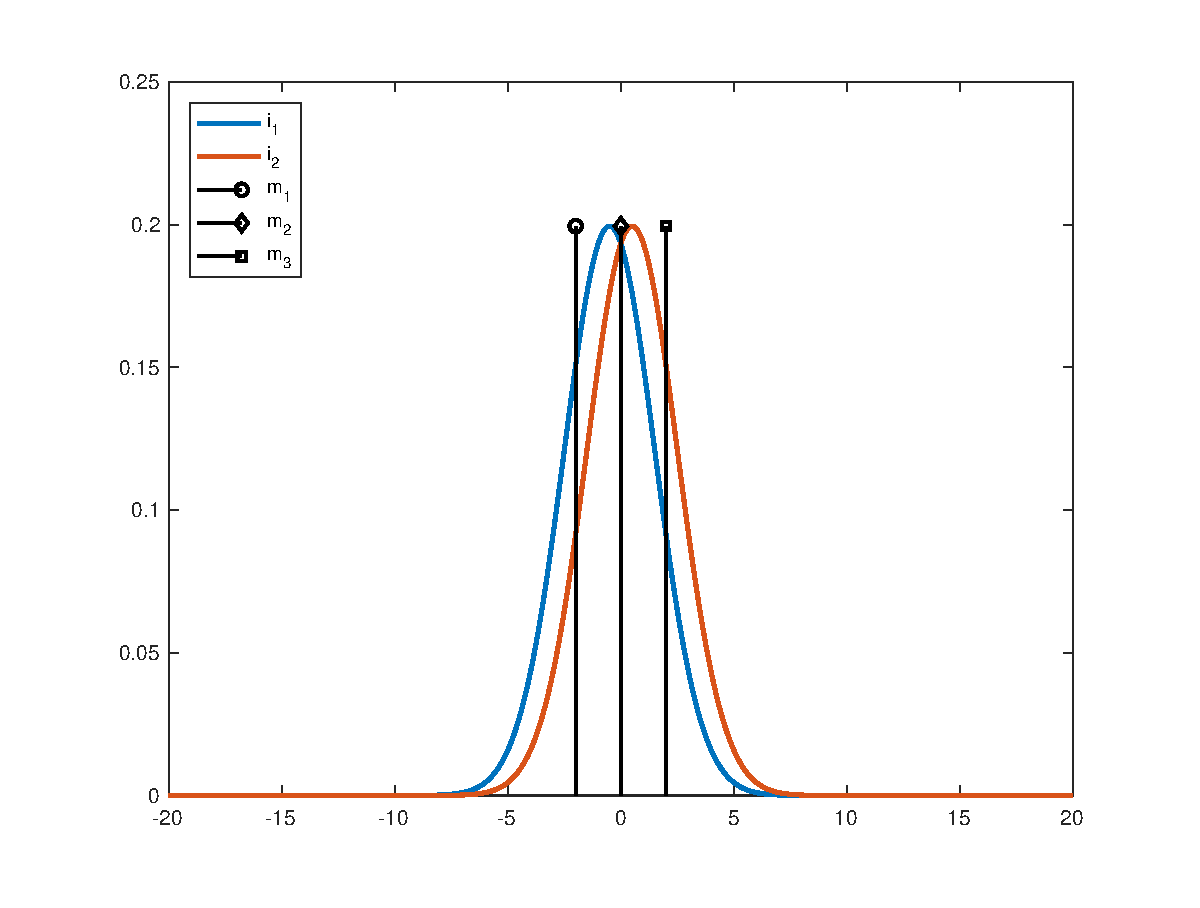
\includegraphics[width = 0.95\columnwidth]{example-existrack.eps}
%     \caption{Illustrative example with two target densities $i_1$ to $i_2$, and three measurements $m_1$ to $m_3$. Note that the association of measurement $m_2$ is ambiguous: is it from target $i_1$ or from target $i_2$? The updated MBM are given in Table \ref{tab:example_existrack}.}
%     \label{fig:existtrackexample}
% \end{figure}

% \begin{table}[!t]
% \footnotesize
% \caption{An example of how the order of Bernoulli components in each MB of the updated MBM changes from one iteration to next, for the scenario in Fig. \ref{fig:existtrackexample}.}
% \label{tab:example_existrack}
% \centering
% 	\begin{tabular}{c|l l l}
% % 	\vskip 1pt
% 		Asso&Weight&MB at iteration $t$& MB at iteration $t+1$\\
% 		\hline
% 		$A_1$&$\mathcal{W}^1=0.03$&$f^{1,1}_{\emptyset}, f^{1,2}_{\{m_1,m_2,m_3\}}$&$f^{1,1}_{\emptyset}, f^{1,2}_{\{m_1,m_2,m_3\}}$\\
% 		&&&\\
% 		$A_2$&$\mathcal{W}^2=0.24$&$f^{2,1}_{\{m_1\}}, f^{2,2}_{\{m_2,m_3\}}$&$f^{2,1}_{\{m_1\}}, f^{2,2}_{\{m_2,m_3\}}$\\
% 		&&&\\
% 		$A_3$&$\mathcal{W}^3=0.14$&$f^{3,1}_{\{m_2\}}, f^{3,2}_{\{m_1,m_3\}}$&$f^{3,1}_{\{m_2\}}, f^{3,2}_{\{m_1,m_3\}}$\\
% 		&&&\\
% 		$A_4$&$\mathcal{W}^4=0.09$&$\boldsymbol{f^{4,1}_{\{m_3\}}, f^{4,2}_{\{m_1,m_2\}}}$&$\boldsymbol{f^{4,2}_{\{m_1,m_2\}},f^{4,1}_{\{m_3\}}}$\\
% 		&&&\\
% 		$A_5$&$\mathcal{W}^5=0.24$&$f^{5,1}_{\{m_1,m_2\}}, f^{5,2}_{\{m_3\}}$&$f^{5,1}_{\{m_1,m_2\}}, f^{5,2}_{\{m_3\}}$\\
% 		&&&\\
% 		$A_6$&$\mathcal{W}^6=0.14$&$f^{6,1}_{\{m_1,m_3\}}, f^{6,2}_{\{m_2\}}$&$f^{6,1}_{\{m_1,m_3\}}, f^{6,2}_{\{m_2\}}$\\
% 		&&&\\
% 		$A_7$&$\mathcal{W}^7=0.09$&$\boldsymbol{f^{7,1}_{\{m_2,m_3\}}, f^{7,2}_{\{m_1\}}}$&$\boldsymbol{f^{7,2}_{\{m_1\}},f^{7,1}_{\{m_2,m_3\}}}$\\
% 		&&&\\
% 		$A_8$&$\mathcal{W}^8=0.03$&$f^{8,1}_{\{m_1,m_2,m_3\}}, f^{8,2}_{\emptyset}$&$f^{8,1}_{\{m_1,m_2,m_3\}}, f^{8,2}_{\emptyset}$\\
% % 		\vskip 1pt
% % 		\hline
% 	\end{tabular}
% \end{table}

% \begin{figure}[!t]
%     \centering
%     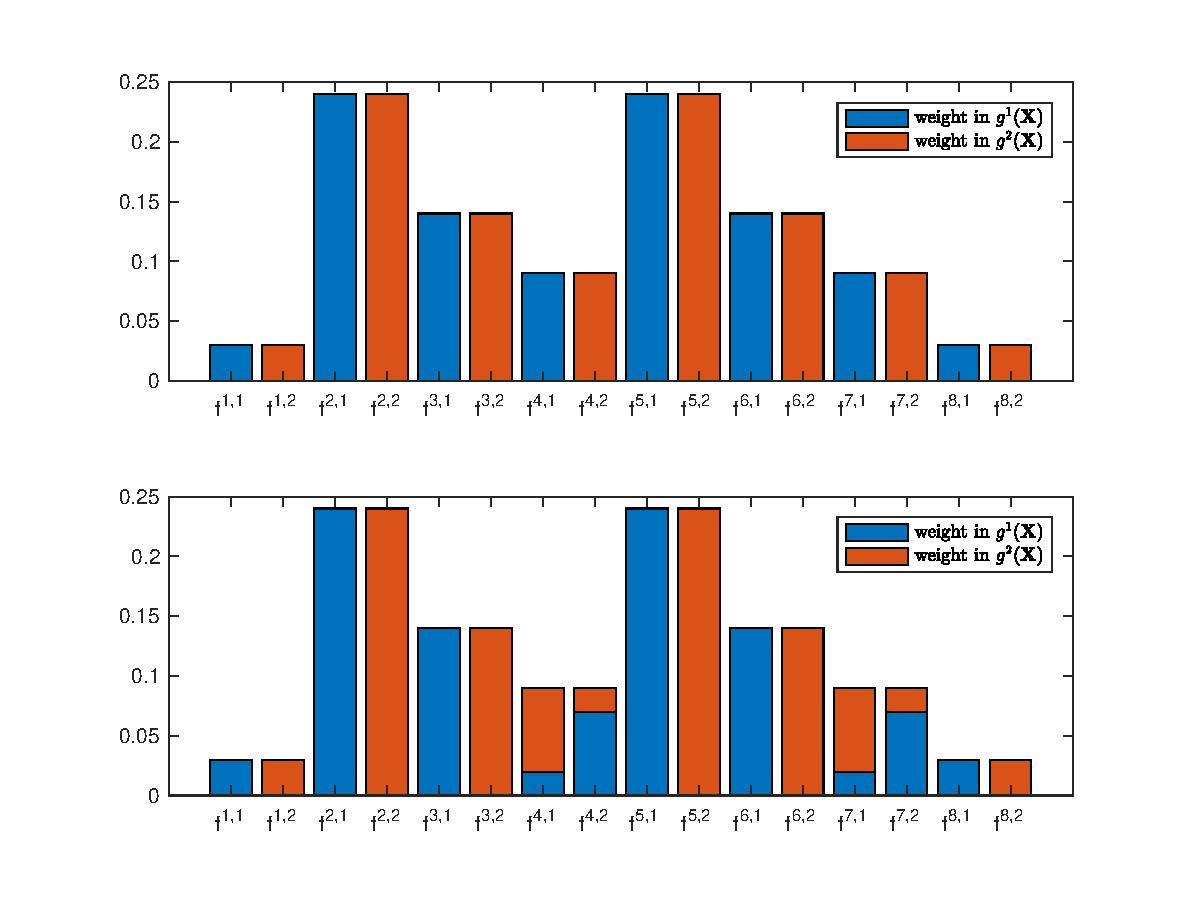
\includegraphics[width = \columnwidth]{example_eafs.eps}
%     \caption{An example of how the weight of single target hypothesis density $f^h(\mathbf{X})$ in the new approximated Bernoulli component $g^1(\mathbf{X})$ and $g^2(\mathbf{X})$ changes from one iteration (top) to next (bottom), for the scenario in Fig. \ref{fig:existtrackexample}.}
%     \label{fig:existtrackexample_eafs}
% \end{figure}

% % \newtheorem{example}{Example}

% \begin{example}
% \emph{Consider a one-dimensional scenario where there are two existing target denoted $i_1$ to $i_2$, and three measurements denoted $m_1$ to $m_3$. We assume that all the measurements come from existing targets. In this case there are eight possible data associations $A_i$, for the sake of simplicity indexed $i$ from 1 to 8. Note that the order of the associations does not have a specific meaning; one was simply chosen for the illustration.}

% \emph{One realization of such a scenario is shown in Fig. \ref{fig:existtrackexample}, where the target density and the measurements are shown. The subscript of each Bernoulli component indicates the measurement cell the corresponding target is associated to, shown in Table \ref{tab:example_existrack}. Bernoulli components in the same column correspond to the same track, and each track, in this case, consists of eight single target hypotheses. The weight of each single target hypothesis density in the each approximated Bernoulli component is shown in Fig. \ref{fig:existtrackexample_eafs}. Because there are sixteen single target hypotheses and two tracks, the assignment weight matrix has sixteen rows and two columns accordingly. In this scenario, target $i_1$ and target $i_2$ are closed spaced, and the association of measurement $m_2$ is ambiguous: is measurement $m_2$ from target $i_1$ or target $i_2$? }

% \emph{Let us first consider the illustration of the variational MB algorithm based on optimal assignment. Given an MBM at iteration $t$, the approximated MB can be obtained by merging Bernoulli components that are assigned to the same target. Further, given an approximated MB at iteration $t+1$, we can permute the order of Bernoulli components and find the optimal permutation for each MB according to the E-step (\ref{eq:estepoptimal}). Assume that, in this case, Bernoulli density $f^{4,2}_{\{m_1,m_2\}}(\mathbf{X})$ is closer to the approximated density of target $i_1$ than the approximated density of target $i_2$ , and that Bernoulli density $f^{4,1}_{\{m_3\}}(\mathbf{X})$ is closer to the approximated density of target $i_2$ than the approximated density of target $i_1$. The same also holds for Bernoulli densities $f^{7,1}_{\{m_2,m_3\}}(\mathbf{X})$ and $f^{7,2}_{\{m_1\}}(\mathbf{X})$. In order to minimize the upper bound of (\ref{eq:vaorigin}), the order of Bernoulli components in the fourth and the seventh MB should be flipped. After reordering, we can obtain our new approximated MB by merging Bernoulli components according to their new assignments at iteration $t+1$.}

% \emph{The variational MB algorithm based on efficient approximation of feasible set is illustrated in Fig. \ref{fig:existtrackexample_eafs}. Each bar represents the total weight of a single target hypothesis density that is assigned to the two approximated Bernoulli components, and the weight proportion is represented by two different colours. In order to minimize the upper bound of (\ref{eq:vaorigin}), a proportion of the weights of assigning $f^{4,1}(\mathbf{X})$ and $f^{7,1}(\mathbf{X})$ to $g^1(\mathbf{X})$ should be shifted to $g^2(\mathbf{X})$, and a proportion of the weights of assigning $f^{4,2}(\mathbf{X})$ and $f^{7,2}(\mathbf{X})$ to $g^2(\mathbf{X})$ should be shifted to $g^1(\mathbf{X})$ accordingly. Note that, due to the constraints specified in the approximated set of missing data distribution (\ref{eq:polytope}), the sum of the weights of assigning different single target hypotheses to the same approximated Bernoulli component and the sum of the weights of assigning the same single target hypothesis to different approximated Bernoulli components should remain unchanged from iteration $t$ to iteration $t+1$. }
% \\\IEEEQEDopen
% \end{example}

% \begin{figure}[!t]
%   \begin{minipage}[b]{0.5\columnwidth}
%     \centering
%     \begin{tabular}{l l l l l }
% 	\hline
% % 	\vskip 1pt
% 		$f^{1,1}$ &   &$f^{1,2}$ &   &  $\mathcal{W}^1$\\
% 		$f^{2,1}$   &   &$f^{2,2}$ &   & $\mathcal{W}^2$\\
% 		$f^{3,1}$ &   & $f^{3,2}$ &   & $\mathcal{W}^3$\\
% 		$f^{4,1}$ &   &$f^{4,2}$ &   &  $\mathcal{W}^4$\\
% 		$f^{5,1}$   &   &$f^{5,2}$ &   & $\mathcal{W}^5$\\
% 		$f^{6,1}$ &   & $f^{6,2}$ &   & $\mathcal{W}^6$\\
% 		$f^{7,1}$ &   &$f^{7,2}$ &   &  $\mathcal{W}^7$\\
% 		$f^{8,1}$   &   &$f^{8,2}$ &   & $\mathcal{W}^8$\\
% % 		\vskip 1pt
% 		\hline
% 	\end{tabular}
%   \end{minipage}%
%   \begin{minipage}[b]{0.5\columnwidth}
%     \centering
% \begin{tabular}{l l l l l}
% 	\hline
% % 	\vskip 1pt
% 		$f^{1,1}$ &   &$f^{1,2}$ &   & $\mathcal{W}^1$\\
% 		$f^{2,1}$   &   &$f^{2,2}$ &   & $\mathcal{W}^2$\\
% 		$f^{3,1}$ &   & $f^{3,2}$ &   & $\mathcal{W}^3$\\
% % 		\vskip 1pt
% 		\hline
% 	\end{tabular}
% \end{minipage}
% \caption{The order of Bernoulli components in each MB of the updated MBM from one iteration (left) to next (right), for the scenario in Fig. \ref{fig:existtrackexample}.}
% \label{fig:example_existrack}
% \end{figure}


% ~\\
% \indent
% It was revealed in \cite{variational} that the minimisation of the upper bound (\ref{eq:vaorigin}) can be solved approximately as
% \begin{equation}
% \operatornamewithlimits{argmin}_{q(h,i)\in\mathcal{M}}-\sum_{i=1}^N\int\bigg(\sum_{h\in\mathcal{H}}q(h,i)f^h(\mathbf{X})\bigg)\log g^i(\mathbf{X})\delta\mathbf{X},
% \label{eq:feasibleset}
% \end{equation}
% where $\mathcal{H}$ is the set of single target hypotheses, $q(h,i)$ is a simplified representation of $q_j(\pi^j)$, which specifies the weight of single target hypothesis density $f^h(\mathbf{X})$ in the new Bernoulli component $g^i(\mathbf{X})$, and the feasible set $\mathcal{M}$ is an approximation needed for tractability
% \begin{multline}
%     \mathcal{M} = \Bigg\{q(h,i)\geq0\Bigg|\sum_{h\in\mathcal{H}}q(h,i)=1 ~\forall~ i\in\{1,...,N\},\\\sum_{i=1}^Nq(h,i)=p_h ~\forall~ h\in\mathcal{H}\Bigg\}.
%     \label{eq:polytope}
% \end{multline}
% The constraint $p_h$ satisfies $p_h=\sum_{i=1}^Np_i(h)$, where
% \begin{equation}
% p_i(h) = \sum\limits_{f^j(\mathbf{X})|f^{j,i}(\mathbf{X})=f^h(\mathbf{X})}\mathcal{W}^j.
% \label{eq:marginalprob}
% \end{equation}
% The derivation of (\ref{eq:feasibleset}) can be found in \cite{variational}. Note that here the missing data distribution is no longer constrained to vary only with the global hypotheses. In this case, each approximated Bernoulli component can be expressed as the weighted sum of different single target hypothesis densities, and the M-step becomes
% \begin{equation}
% g^i(\mathbf{X}) = \sum_{h\in\mathcal{H}}q(h,i)f^h(\mathbf{X}),
% \end{equation}
% while the E-step reverts to a LP:
% \begin{equation}
% \operatornamewithlimits{argmin}_{q(h,i)}\sum_{h\in\mathcal{H}}\sum_{i=1}^N-q(h,i)\int f^h(\mathbf{X})\log g^{i}(\mathbf{X})\delta \mathbf{X},
% \label{eq:esteplp}
% \end{equation}
% \begin{align*}
%     \text{subject to   } &\sum_{i=1}^Nq(h,i) = p_h~\forall~h,\\
%     &\sum_{h\in\mathcal{H}}q(h,i) = 1~\forall~i,\\
%     &q(h,i) \geq 0~\forall~h,i.
% \end{align*}
% Problem of this type can be solved using methods such as the simplex algorithm. The resulting algorithm can be initialised with $q(h,i)=p_i(h)~\forall~h,i$.
\begin{table}[!t]
\footnotesize
\caption{Pseudo Code of New Tracks Forming}
\label{pmbnewtracks}
\centering
\begin{tabular}{cr}
  \hline
  \begin{minipage}{0.43\textwidth}
  \vskip 1pt
\begin{algorithmic}
\renewcommand{\algorithmicrequire}{\textbf{Input:}}
\renewcommand{\algorithmicensure}{\textbf{Output:}}
\REQUIRE{$\{(\mathcal{W}^j, \{f^{j,i}(\mathbf{X}^i)\}_{i\in\mathbb{I}^j\setminus\mathbb{I}})\}_{j\in\mathbb{J}}$, merging threshold $\tau$}
\ENSURE{$\{g^{\iota}(\mathbf{X}^{\iota})\}_{\iota\in\hat{\mathbb{I}}\setminus\mathbb{I}}$}
\STATE Sort $f^j(\mathbf{X})$ in the descending order of $\mathcal{W}^j$;
% \STATE Prune $f^j(\mathbf{X})$ with negligible $\mathcal{W}^j$ to get truncated $f^j(\mathbf{X})$, where $j\in\hat{\mathbb{J}}$;
\STATE $I \leftarrow 0$;
\STATE $\hat{\mathbb{I}} \leftarrow \mathbb{I}$;
% \STATE $\mathbb{L}^I \leftarrow \emptyset$;
\FORALL{$j=\{1,...,|\mathbb{J}|\}$}
\IF{$|\mathbb{I}^j|>|\mathbb{I}|$}
\FORALL{$i=\{|\mathbb{I}|+1,...,|\mathbb{I}^j|\}$}
\IF{$(j,i)\notin\mathbb{L}^l~\forall~l=\{1,...,I\}$}
\STATE $I \leftarrow I + 1$;
\STATE $\mathbb{L}^I \leftarrow \mathbb{L}^I\cup\{(j,i)\}$;
\STATE $\hat{\mathbb{I}} \leftarrow \mathbb{I}\cup \{|\mathbb{I}|+I\}$;
\ENDIF
\FORALL{$j^+=\{j+1,...,|\mathbb{J}|\}$}
\FORALL{$i^+=\{|\mathbb{I}|+1,...,|\mathbb{I}^{j^{+}}|\}$}
\IF{$(j,i)\notin\mathbb{L}^l~\forall~l\in\{1,...,I\}$}
\STATE 
    $d^{i^+}\leftarrow D_{\text{SKL}}\big(f^{j,i}(\mathbf{X})||f^{j^+,i^+}(\mathbf{X})\big)$;
\ENDIF
\ENDFOR
\STATE $[d^*,i^*] \leftarrow \min(d)$;
\IF{$d^*<\tau$}
\STATE $\mathbb{L}^I \leftarrow \mathbb{L}^I\cup\{(j^+,i^*)\}$;
\ENDIF
\ENDFOR
\ENDFOR
\ENDIF
\ENDFOR
\FORALL{$\iota=\{|\mathbb{I}|+1,...,|\hat{\mathbb{I}}|\}$}
\STATE Calculate $g^{\iota}(\mathbf{X}^{\iota})$ using (\ref{eq:approxnewtrack}).
\ENDFOR
\end{algorithmic}
\vskip 3pt
 \end{minipage}
 &\\
  \hline
 \end{tabular}
\end{table}

\subsection{New track formation}
\label{section:newtracks}
% A big barrier in the extended target PMB filter is the formation of new tracks. In point target tracking, a new track is created for each measurement. Given $|\mathbf{Z}|$ measurements, there are $|\mathbf{Z}|$ mutually independent possible new tracks. The new tracks can be formed out of the marginal association probabilities (cf. (\ref{eq:marginalprob})) \cite{pmbmpoint}. 
% Denote the Bernoulli density of the track generated by the $z$th measurement as $f^{N+z}(\mathbf{X})$, where $z\in\{1,...,|\mathbf{Z}|\}$, then the existence probability of the $z$th new track satisfies
% \begin{equation}
%     \hat{r}^{N+z} = r^{N+z} \sum_{f^j(\mathbf{X})|f^{j,i}(\mathbf{X})=f^{N+z}(\mathbf{X})} \mathcal{W}^j.
% \end{equation}
% In extended target tracking, measurements are partitioned into measurement cells and a new track is created for each measurement cell. Given $|\mathbf{Z}|$ measurements, there are $2^{|\mathbf{Z}|}-1$ possible ways in which we can form a subset of measurements. Each such subset can, in an association, be associated to a new target. This means that in extended target tracking, the updated MBM can at most contain $2^{|\mathbf{Z}|}-1$ different possible new targets. Let $N_+^j$ denote the number of measurement cells in the $j$th updated global hypothesis. According to the definition of track, there are $N_+^j$ new tracks created, but only $N_+^j-N$ of them, which are associated to newly detected targets, have valid existence probability in the $j$th global hypothesis. 

% One strategy to form new tracks, which is similar to \cite{pmbmpoint}, is only to merge single target hypotheses across different global hypotheses that are created by the same measurement cell and treat each different single target hypothesis as a candidate for a potential new target. In order words, the existence probability of new track created by measurement cell $\mathbf{C}$ is determined by summing over the data association hypotheses where $\mathbf{C}$ is associated to the background. This approach is simple to implement; nevertheless, it has several drawbacks. First, a large number of new tracks with low existence probability can be created using this approach. Second, this approach approximates new tracks generated by different measurement cells as independent. But if some of the measurement cells have shared measurements, which is the typical case, there might be a high dependency between the new tracks that are created by these measurement cells. This is not consistent with the assumption that tracks are independent.

We present a greedy method to form new tracks in a reasonable and efficient way. The pseudo code of this merging approach is given in Table \ref{pmbnewtracks}. The intuition behind this proposed method is that we want to merge highly dependent Bernoullis across different MBs so that similar new tracks will not be formed in the same local region and new tracks with significant different Bernoulli densities will not be merged.

In this merging approach, we only merge Bernoullis in different MBs that are considered similar enough. For any pair of Bernoulli densities, the symmetrised KL divergence is used to measure the similarity \cite{ArdeshiriGOO:2015}, defined as
\begin{equation}
    D_{\text{SKL}}(p||q) = D_{\text{KL}}(p||q) + D_{\text{KL}}(q||p). 
\end{equation}

To start with, the MB densities are sorted in the descending order of their weights, so that $f^1(\mathbf{X})$ has the highest weight. Remember that reordering the MBs will not change the MBM process. Then, we cluster Bernoullis that satisfy the merging criteria into the same group. As a result, the number of new tracks formed is equal to the number of Bernoulli clusters. Lastly, new tracks are formed by only merging Bernoullis within the same group. For the $\iota$th ($\iota\in\hat{\mathbb{I}}\setminus\mathbb{I}$) new track in the approximated MB $g(\mathbf{X})$, its Bernoulli density can be expressed as
\begin{equation}
    g^{\iota}(\mathbf{X}^\iota) \propto \sum_{j\in\mathbb{J}}\mathcal{W}^j\sum_{i\in\mathbb{I}^j\setminus\mathbb{I}}f^{j,i}(\mathbf{X})\Delta_{\{(j,i)\}\in\mathbb{L}^{\iota-|\mathbb{I}|}}, \iota\in\hat{\mathbb{I}}\setminus\mathbb{I},
    \label{eq:approxnewtrack}
\end{equation}
where set $\mathbb{L}^{\iota-|\mathbb{I}|}$ contains indices of Bernoullis that are within the same group. Empirical results show that the number of tracks formed using this approach can be kept to a relatively small number. We illustrate this with the following example. 

\begin{example}
\emph{Consider the same scenario illustrated in Fig. \ref{fig:example}. There are five new tracks created in total in the three global hypotheses. If we assume that Bernoulli densities of these five new tracks are mutually independent, it is likely that none of these tracks are detected by the estimator due to their low existence probabilities.} 

\emph{Following the proposed merging approach, we start by merging $f^{1,3}(\mathbf{X}^3)$ with $f^{2,3}(\mathbf{X}^3)$ and $f^{3,3}(\mathbf{X}^3)$, due to the small symmetrised KL divergence between the pair $f^{1,3}(\mathbf{X}^3)$, $f^{2,3}(\mathbf{X}^3)$, and between the pair $f^{1,3}(\mathbf{X}^3)$, $f^{3,3}(\mathbf{X}^3)$. Next, we merge $f^{1,4}(\mathbf{X}^4)$ with $f^{2,4}(\mathbf{X}^4)$, due to their high similarity in the sense of symmetrised KL divergence. After merging, the number of Bernoullis in the approximated MB reduces from five to two: $g^3(\mathbf{X}^3)$ has existence probability $\hat{r}^3=1$, and $g^4(\mathbf{X}^4)$ has existence probability $\hat{r}^4=0.75$.}
\\\IEEEQEDopen
% \emph{Consider the same scenario illustrated in Fig. \ref{fig:example}. }

% \emph{One realization of such a scenario is shown in Fig. \ref{fig:newtrackexample}, where the target density and the measurements are shown. In this case only four associations have significant weights; these four associations are given in Table \ref{tab:newtrackexample}. Among these data associations, association $A_9$ and $A_6$ have dominant weights, and they correspond to one highly ambiguous assignment in this scenario: is measurement $m_2$ from existing target $i_1$, or a new target? }

% \emph{Consider the same scenario illustrated in Fig. \ref{fig:example}. Assume that associations with negligible weights are pruned. Because each measurement cell creates a new track, there are seven new tracks created given these four data associations. But only the three tracks created by measurement cell $\{m_3\}, \{m_2,m_3\}, \{m_1,m_3\}$ that are associated to the background have valid existence probability. If we assume that Bernoulli densities of these three new tracks are mutually independent, it is likely that none of these tracks is detected by the estimator due to their low existence probabilities. However, if the Bernoulli densities of the three tracks created by measurement cell $\{m_3\}, \{m_2,m_3\}, \{m_1,m_3\}$ are merged because of the small symmetrised KL divergence between the pair $\{m_3\}, \{m_2,m_3\}$ and between the pair $\{m_3\}, \{m_1,m_3\}$, the existence probability of the approximated Bernoulli component would be $0.88$, which means that the new born target has a very high chance to be detected. After merging, the number of Bernoulli components in the approximated MB reduces from four to two.}
\end{example}

% \begin{figure}[!t]
%     \centering
%     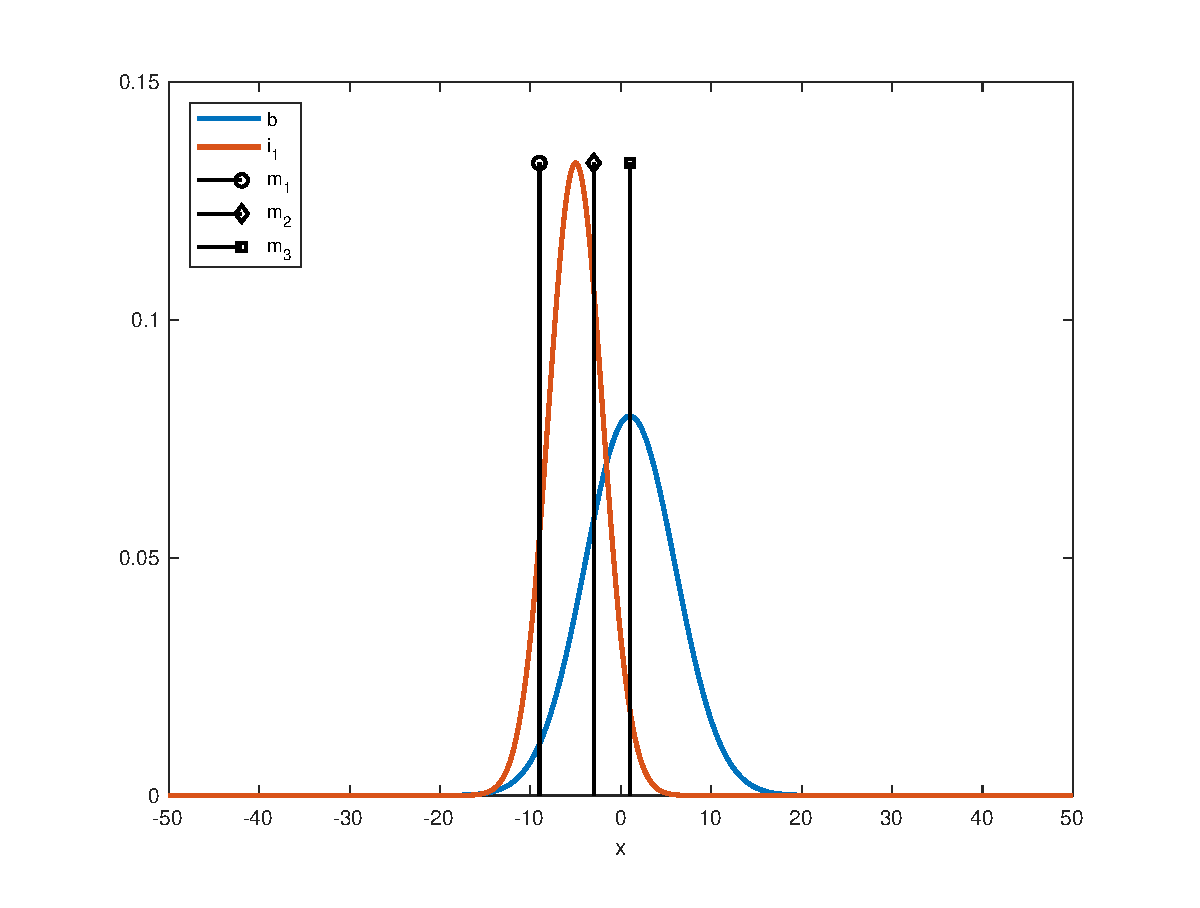
\includegraphics[width = 0.95\columnwidth]{example_newtrack.eps}
%     \caption{Illustrative example with a single target density $i_1$, a PPP intensity $b$ for the background (new object or clutter), and three measurements $m_1$ to $m_3$. Note that the association of measurement $m_2$ is ambiguous: is it from target $i_1$ or from the background $b$? The corresponding significant associations are given in Table \ref{tab:newtrackexample}.}
%     \label{fig:newtrackexample}
% \end{figure}

% \begin{table}[!t]
% \footnotesize
% \caption{The four most significant associations, and their corresponding weights, for the scenario in Figure \ref{fig:newtrackexample}}
% \label{tab:newtrackexample}
% \centering
% 	\begin{tabular}{l l l l l}
% 	\hline
% % 	\vskip 1pt
% 		$A_9:$ &   &$\{i_1,m_1,m_2\}, \{m_3\}$ &   & $\mathcal{W}^{A}=0.46$\\
% 		$A_6:$   &   &$\{i_1,m_1\}, \{m_2,m_3\}$ &   & $\mathcal{W}^{A}=0.37$\\
% 		$A_{15}:$ &   & $\{i_1,m_1,m_2,m_3\}$ &   & $\mathcal{W}^{A}=0.12$\\
% 		$A_7:$ &   & $\{i_1,m_2\}, \{m_1,m_3\}$ &   & $\mathcal{W}^{A}=0.05$\\
% % 		\vskip 1pt
% 		\hline
% 	\end{tabular}
% \end{table}


\section{GGIW Implementation}
Solving the multiple extended target tracking problem requires not only a multiple target tracking framework, but also a single extended target model. For the modelling of the spatial distribution, two popular models are the Random Hyper-surface Models \cite{hypersurface} and the Gaussian inverse Wishart (GIW) approach \cite{randomMatrix,randomMatrix2}. The former is designed for general star-convex shape; the latter relies on the elliptic shape and it models the spatial distribution of target-generated measurements as Gaussian with unknown mean and covariance. The Gamma GIW (GGIW) model \cite{phdextended,cphdextended} is an extension of the GIW model that incorporates the estimation of target measurement rate.

In this section, some implementation details of the PMB filter are presented. A GGIW implementation of the PMBM filter has been given in \cite{pmbmextended2}. To make the comparison easy, we choose to use the GGIW model, in which the target shape is approximated as an ellipse, and the target measurement rate is modelled as a Poisson random variable. In addition, we present strategies regarding how to address the third challenge in an MBM approximation that we outlined in Section \ref{section:challenge}, i.e., the merging of a selection of Bernoullis, under a GGIW model. 

% There are several single extended target models available in the literature, see \cite{extendedoverview} for an overview. 

\subsection{Single target models}
In the GGIW model, it is assumed that the measurements are Gaussian distributed around the centroid of the target. The extended target state $\mathbf{x}_k$ is the combination of a random Poisson rate $\gamma_k$ modelling the average number of measurements generated by the target, a random vector $\xi_k$ describing the target kinematic state, and a random matrix $\chi_k$ describing the target size and shape, i.e., $\mathbf{x}_k=\{\xi_{k},\chi_{k},\gamma_{k}\}$.

The motion models are given by
\begin{subequations}
\begin{align}
    \xi_{k+1} &= F(\xi_k) + w_k,\\
    \chi_{k+1} &= M(\xi_k)\chi_kM(\xi_k)^T,\\
    \gamma_{k+1} &= \gamma_k,
\end{align}
\end{subequations}
where $F(\cdot)$ is a motion model, $w_k$ is a zero mean Gaussian noise and $M(\cdot)$ is a transformation matrix. 

The measurement likelihood for a single measurement $\mathbf{z}$ is
\begin{equation}
    \phi(\mathbf{z}_k|\mathbf{x}_k) = \mathcal{N}(\mathbf{z}_k;H_k\xi_k,\chi_k+R_k),
    \label{eq:mealikelihood}
\end{equation}
where $H_k$ is the measurement model, and $R_k$ is the covariance of a zero mean Gaussian noise. The single target conjugate prior for the PPP model (\ref{eq:ppp}) with single measurement
likelihood (\ref{eq:mealikelihood}) is a GGIW distribution \cite{randomMatrix,randomMatrix2}
\begin{multline}
f(\mathbf{x}) = \mathcal{GAM}(\gamma;a,b)\mathcal{N}(\xi;m,P)\\ \times\mathcal{IW}_d(\chi;v,V) \triangleq \mathcal{GGIW}(\mathbf{x};\zeta),
\end{multline}
where $\zeta = \{a,b,m,P,v,V\}$ is the set of GGIW density parameters. If we have a PPP birth with GGIW density, then the undetected PPP will have GGIW density, as well as all the Bernoulli components \cite{pmbmextended2}.

\subsection{MBM merging}
The GGIW implementations regarding the prediction and update of PPP and Bernoulli components are not presented due to page limits. The reader is referred to \cite{pmbmextended,pmbmextended2} for more details. In this subsection, we present the GGIW implementations regarding the block coordinate descent used to merge the MBM representing pre-existing tracks. The time index is omitted for simplicity.

\subsubsection{E-step}
In order to solve the optimization problems (\ref{eq:esteplp}) and (\ref{eq:estepoptimal}) of the E-step, the cross entropy between two Bernoulli-GGIW distributions needs to be calculated. Since the gamma distributions, the Gaussian distributions and the inverse Wishart distributions are mutually independent, a tractable solution can be analytically derived. Corresponding mathematical expressions are not presented here due to page limits. 
% See Appendix \ref{appendix:crossentropy} for details.

\subsubsection{M-step}
Given a Bernoulli-GGIW mixture, the existence probability of the approximated Bernoulli is a weighted sum of the existence probabilities of each Bernoulli. Suppose that we have a number of Bernoullis indexed by $n\in\mathbb{N}$, each of which has existence probability $r^n$ and GGIW density $\mathcal{GGIW}(\mathbf{x}^n;\zeta^n)$. The existence probability of the approximated Bernoulli can be
expressed as
\begin{equation}
    \hat{r} = \sum_{n\in\mathbb{N}} w^nr^n,
\end{equation}
% \begin{subequations}
% \begin{align}
%     \hat{r} &= \sum_{n\in\mathbb{N}} w^nr^n,\\
%     f(\hat{\mathbf{x}}) &= \sum_{n\in\mathbb{N}}w^n\mathcal{GGIW}(\mathbf{x}^n;\zeta^n),
% \end{align}
% \end{subequations}
where $w^n$ is the weight of the $n$th Bernoulli. 

The mixture reduction for multivariate Gaussian distribution is straightforward using standard moment matching, which minimizes the KL-divergence. Theorems describing how a sum of an arbitrary number of Gamma components or inverse Wishart components can be merged into a single Gamma or inverse Wishart component are presented in \cite{phdextended} and \cite{gammareduction}, respectively. They are both performed via analytically minimizing the KL divergence. The same merging techniques also apply to merging the MBM representing new tracks (\ref{eq:approxnewtrack}). The existence-conditioned GGIW density of the approximated Bernoulli can be
obtained by
\begin{equation} \underset{\mathcal{GGIW}(\hat{\mathbf{x}};\hat{\zeta})}{\arg\min}D_{\text{KL}}\bigg(\sum_{n\in\mathbb{N}}w^n\mathcal{GGIW}(\mathbf{x}^n;\zeta^n)\big|\big|\mathcal{GGIW}(\hat{\mathbf{x}};\hat{\zeta})\bigg).
\end{equation}

Empirically, we have found that in extended target filtering with GGIW implementation it is generally not advisable to merge the whole GGIW components. The main reason is the extent state: merging two densities with significantly different extent estimates will result in an approximate density in which the extent estimates are distorted. This problem is exacerbated in the extended PMB filter, since the distorted extent states contained by the approximated single MB can easily lead to poor target state estimations in subsequent time steps.
% which can further lead to poor target state estimations in subsequent time steps.

A simple strategy to handle this problem is to use a criterion for deciding which components should be merged. In this work, the KL divergence is used as the similarity measure between any pair of GGIW distributions. The component with the highest weight $\mathcal{GGIW}(\mathbf{x}^{n^*};\zeta^{n^*})$ is chosen as the comparison baseline, which is merged with all other components $\mathcal{GGIW}(\mathbf{x}^{n};\zeta^{n})$ for which it holds
\begin{equation}
    D_{\text{KL}}(\mathcal{GGIW}(\mathbf{x}^{n^*};\zeta^{n^*})||\mathcal{GGIW}(\mathbf{x}^{n};\zeta^{n})) < \tau,
\end{equation}
where threshold $\tau$ determines which GGIW components are going to be merged. 
In this case, the existence-conditioned PDF of the approximated MB can be obtained by
\begin{multline}
\underset{\mathcal{GGIW}(\hat{\mathbf{x}};\hat{\zeta})}{\arg\min}D_{\text{KL}}\bigg(\sum_{\substack{n\in\mathbb{N}:\\D_{\text{KL}}(\mathcal{GGIW}(\mathbf{x}^{n^*};\zeta^{n^*})\\||\mathcal{GGIW}(\mathbf{x}^n;\zeta^n)) < \tau}}w^n\\\times\mathcal{GGIW}(\mathbf{x}^n;\zeta^n)\big|\big|\mathcal{GGIW}(\hat{\mathbf{x}};\hat{\zeta})\bigg).
\end{multline}

% At this point, we have figured out how to address the third challenge that we outlined in Section \ref{section:challenge}, i.e., the merging of a selection of Bernoullis under a GGIW model. 

% \subsection{Recycling}
% For the approximated MB $g(\mathbf{X})$, the recycling method of \cite{recycle} can be applied to Bernoullis with low existence probability. The recycled components are approximated as being Poisson and are incorporated into the PPP representing undetected targets for generating possible new targets in subsequent steps. 

% % The benefits of recycling in the point target PMBM and PMB filters have been demonstrated in \cite{performanceevaluation}.

% Suppose that a Bernoulli $f(\mathbf{X})$ in the form of (\ref{eq:bernoulli}) is approximated by a PPP
% \begin{equation}
% \tilde{f}(\mathbf{X}) = e^{-u}\prod_{\mathbf{x}\in \mathbf{X}}D(\mathbf{x}).
% \end{equation}
% As shown in \cite[p. 359]{rfs}, it is optimal to set $D(\mathbf{x})=\mu f(\mathbf{x})$ and $\mu=r$. 
% % \begin{subequations}
% % \begin{align}
% %     D(\mathbf{x}) &= \mu f(\mathbf{x}),\\
% %     \mu &= r.
% % \end{align}
% % \end{subequations}
% The value of the KL divergence at this optimal choice is given by
% \begin{equation}
%     D_{\text{KL}}(f(\mathbf{X})||\tilde{f}(\mathbf{X})) = r + (1-r)\log(1-r),
% \end{equation}
% and it is very small for existence probability $r$ less than 0.1 \cite{recycle}. Denote $\mathbb{R}$ as the set of indices of Bernoullis to be recycled. After recycling, the total PPP intensity of undetected targets can be expressed as
% \begin{equation}
%     \hat{D}^u(\mathbf{x}) = D^u(\mathbf{x}) + \sum_{\iota\in\mathbb{R}}r^{\iota}f^{\iota}(\mathbf{x}^{\iota}).
% \end{equation}
% The benefits of recycling in the point target PMBM and PMB filters have been discussed in \cite{performanceevaluation}.
% An additional benefit of recycling in the extended target PMB filter is that we can ensure that only new tracks with relatively high existence probability are formed.

\section{Simulations and Results}
In this section, the results from a Monte Carlo simulation study are presented. A comparison between the PMBM, LMB and $\delta$-GLMB filters in \cite{pmbmextended2} shows that the PMBM filter outperforms the LMB filter and the $\delta$-GLMB filter. Therefore, in the simulation study presented here, we only compare the PMBM filter \cite{pmbmextended,pmbmextended2}, the TO-PMB filter and two variants of the PMB filter with variational approximation, namely one with the most likely assignment (MLA-PMB) and one with the efficient approximation of feasible set (EAFS-PMB). In the TO-PMB filter, the new tracks are formed according to the method presented in Table \ref{pmbnewtracks}. In order to reduce the computational cost of the PMBM filter, the MBs with an equal number of Bernoullis and small symmetrised KL divergence can be merged following a similar approach as the most likely assignment used in the PMB filter \cite{pmbmextended2}. The performance of the PMBM filter without MBM merging is also evaluated.

\subsection{State space model}
Target motion follows a constant velocity model. A two-dimensional Cartesian coordinate system is used to define measurement and target kinematic parameters. The kinematic state is $\xi_k = [\mathbf{p}_k,\mathbf{v}_k]^T$, describing the target's position $\mathbf{p}_k=[p_{x,k},p_{y,k}]$ and velocity $\mathbf{v}_k = [v_{x,k},v_{y,k}]$. The single measurement is  $\mathbf{z}_k=[z_{x,k},z_{y,k}]^T$, where $z_{x,k}$ and $z_{y,k}$ describe the position of the measurement. The motion model $F(\cdot)$ and process noise $Q_k$ are expressed as
\begin{equation*}
    F(\xi_k)=\text{I}_2 \otimes \begin{bmatrix}
        1 & T\\
        0 & 1
    \end{bmatrix}\xi_k, \quad Q_k =  \sigma_v^2\text{I}_2\otimes\begin{bmatrix}
        T^4/4 & T^3/2\\
        T^3/2 & T^2
    \end{bmatrix},
\end{equation*}
where $T=1s$ is the sampling period, and $\sigma_v$ is the standard deviation of velocity noise. The random matrix $V_k$ in the inverse Wishart distribution is two-dimensional. Because the kinematic state motion model is constant velocity, the extent transformation function $M$ is an identity matrix \cite{pmbmextended2}, i.e., $M(\xi_k) = \text{I}_2$. 

\subsection{Performance evaluation}
For GGIW-PMB, the target states are extracted by taking the mean vector of all Bernoullis with existence probability larger than 0.5. For GGIW-PMBM, target state extraction is performed analogously, but only from the MB with the highest weight. The estimation performance is evaluated using the Gaussian Wasserstein distance (GWD) \cite{gwd} integrated into the generalised optimal sub-pattern assignment (GOSPA) metric
\cite{gospa}. The GOSPA metric allows for decomposing the estimation error into location error, missed detection error and false detection error. 
% In the simulations, the GOSPA parameters are set to $\alpha=2, p=1, c=40$. 

\subsection{Simulation study}

Filters are evaluated in four different scenarios. True target trajectories are shown in Fig. \ref{fig:trajectory}. For each scenario, the result is averaged over 100 Monte Carlo trials.

% \begin{figure*}[!t]
% 	\centering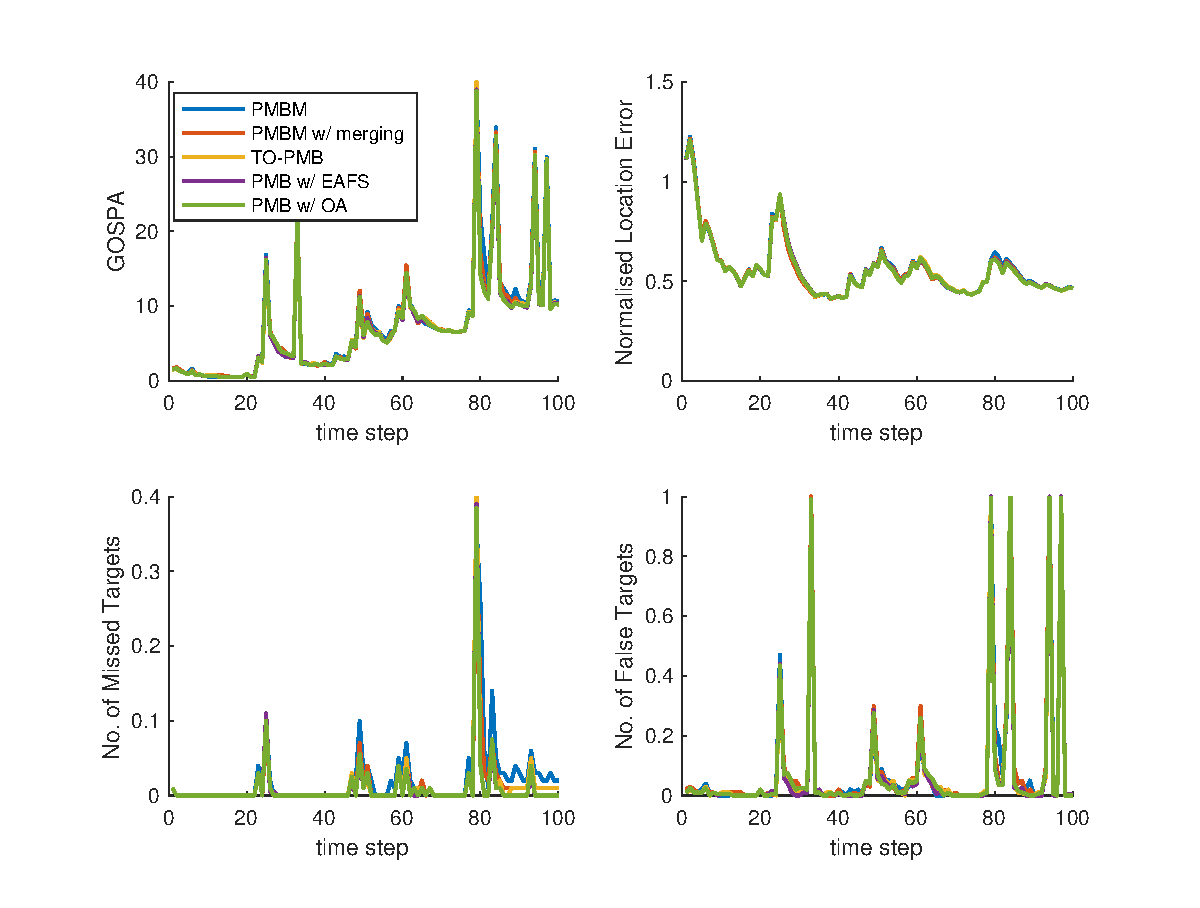
\includegraphics[width = \columnwidth]{GOSPA27Targets3.eps}
% 	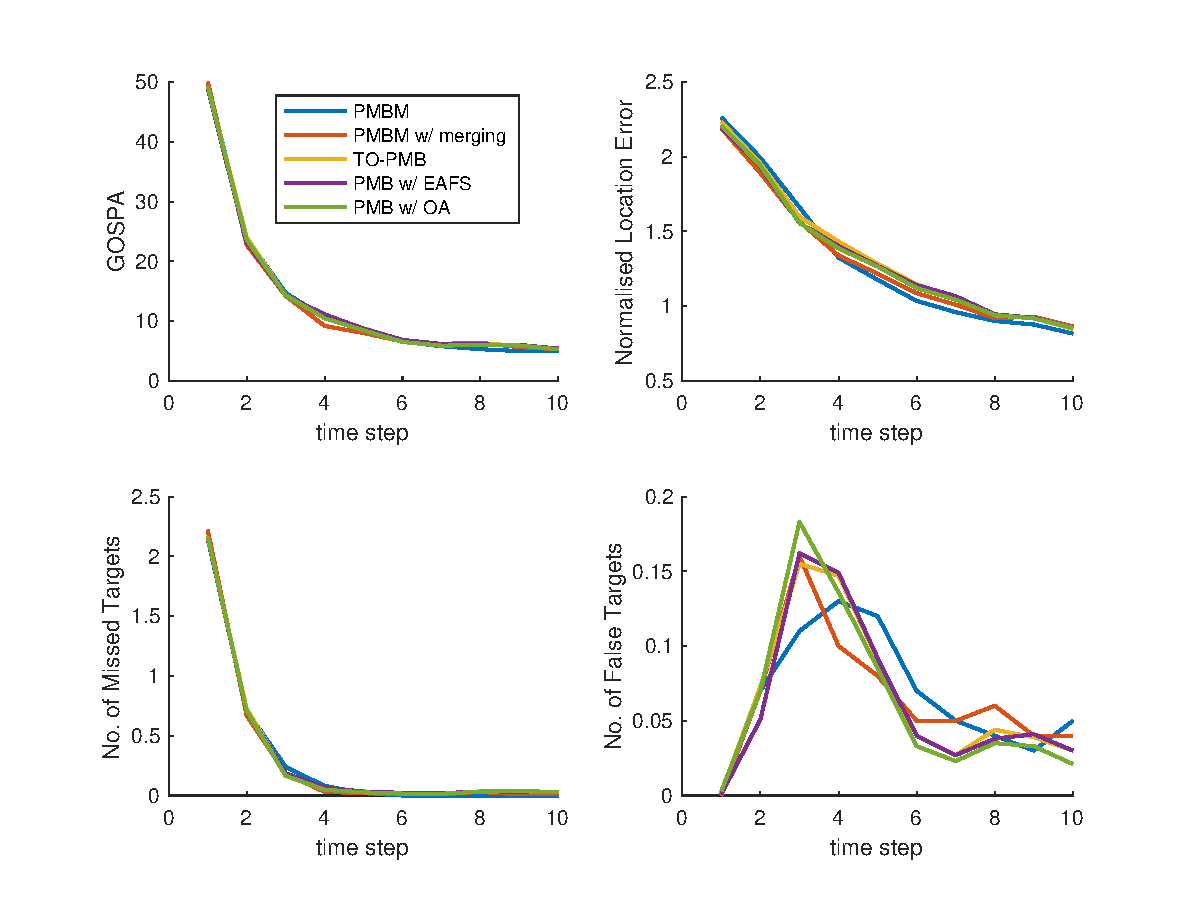
\includegraphics[width = \columnwidth]{GOSPAdenseBirth3.eps}
% 	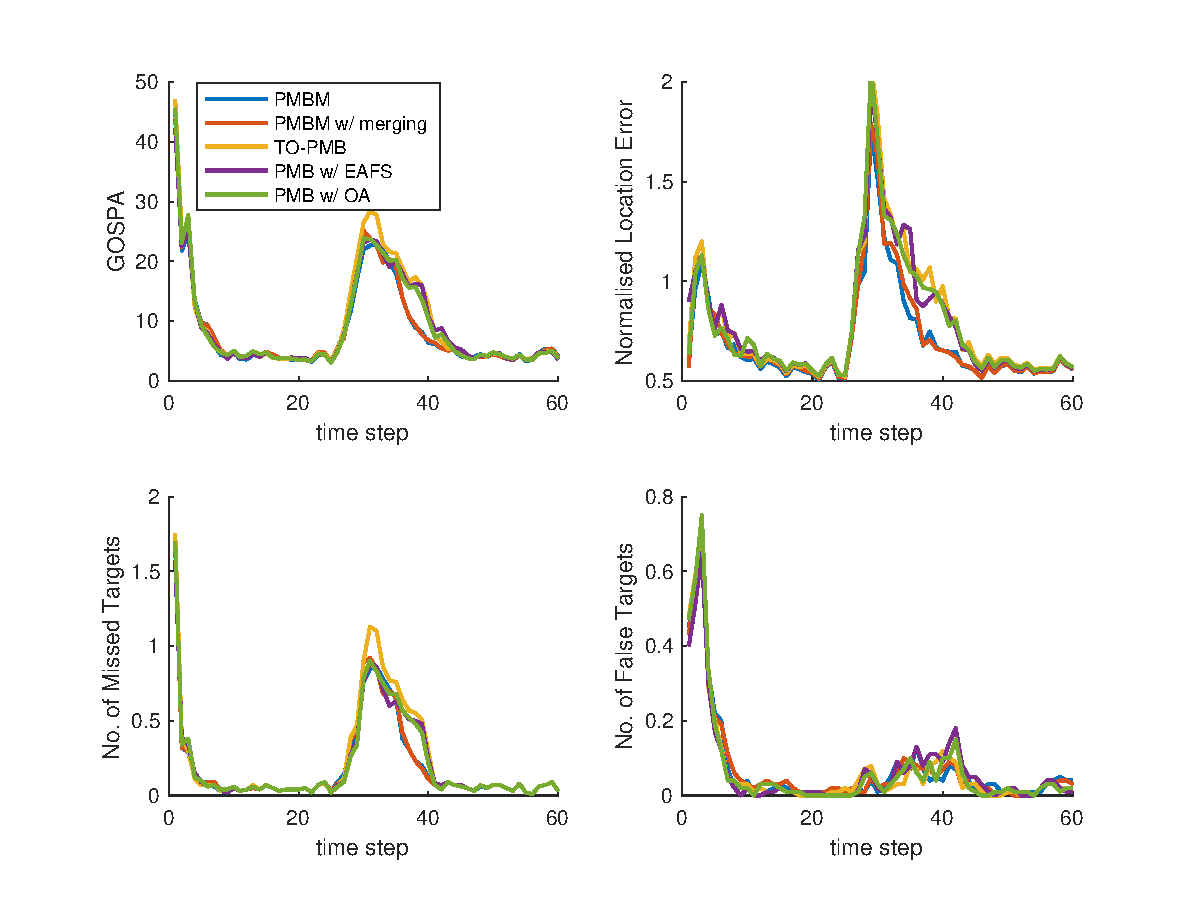
\includegraphics[width = \columnwidth]{GOSPAmergeSplit3.eps}
% 	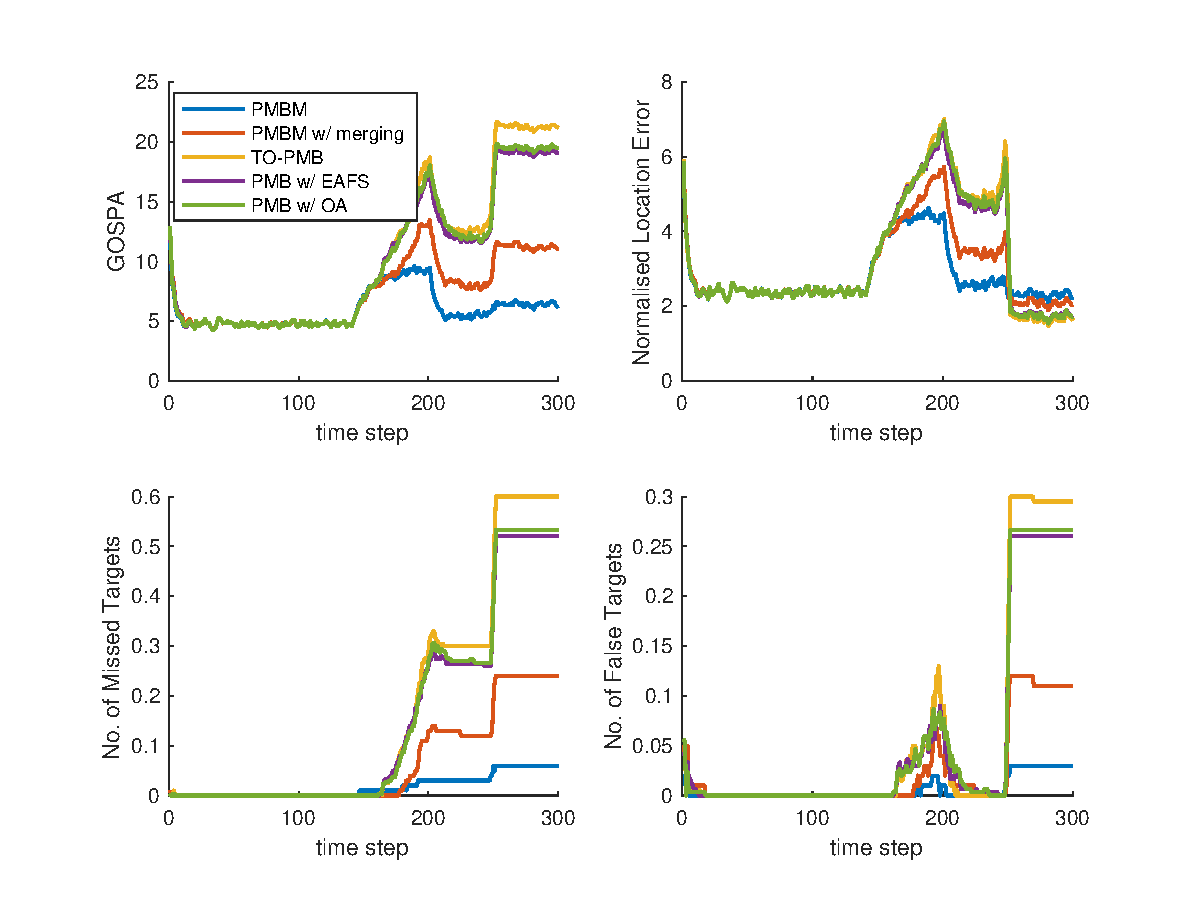
\includegraphics[width = \columnwidth]{GOSPAparallelTurn3.eps}
% 	\caption{Results from simulation of four scenarios, from left to right, top to bottom: 1) 27 targets, 2) dense birth, 3) merge/split and 4) parallel maneuver.}%Overall \textsc{mhg} and \textsc{so} have best performance.
% 	\label{fig:SimulationResults}
% \end{figure*}
\begin{figure}[!t]
\centering
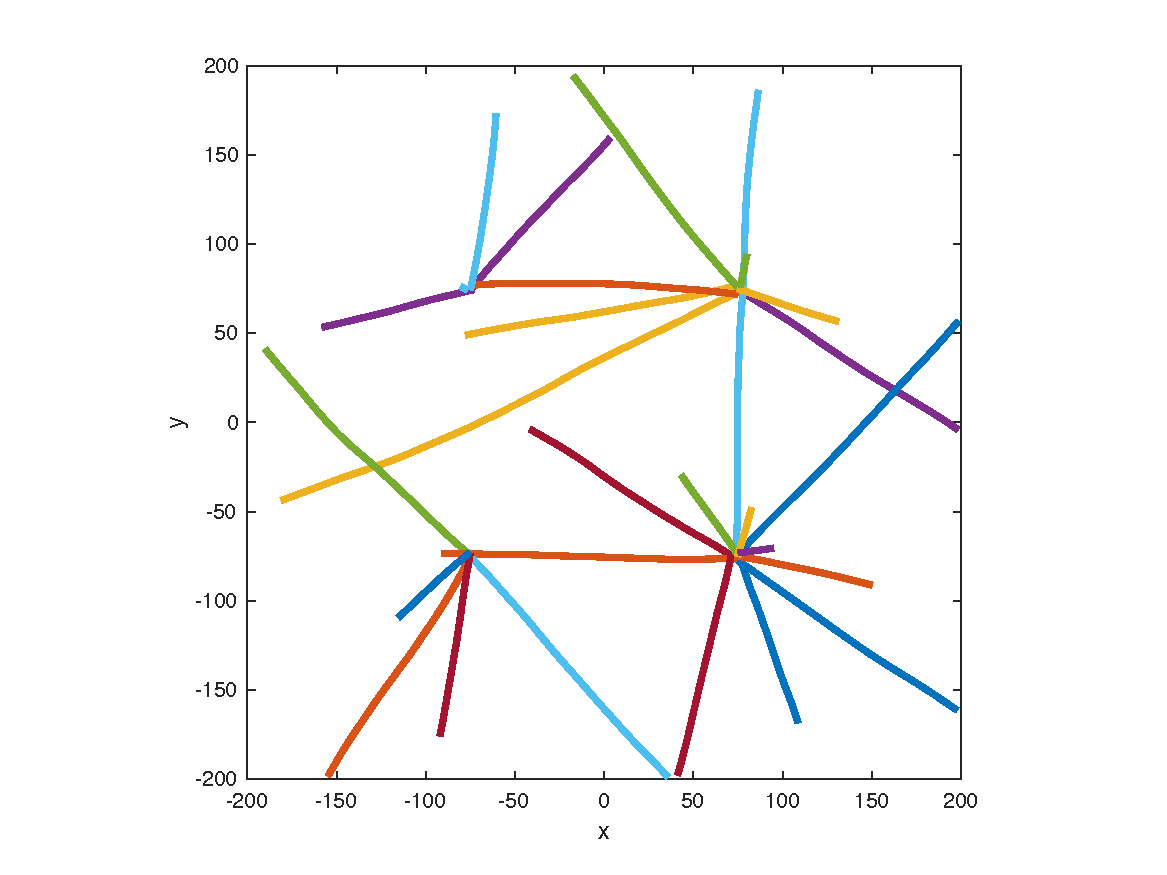
\includegraphics[width=0.24\columnwidth]{trajectory1copy.pdf}
% \hspace{-6mm}
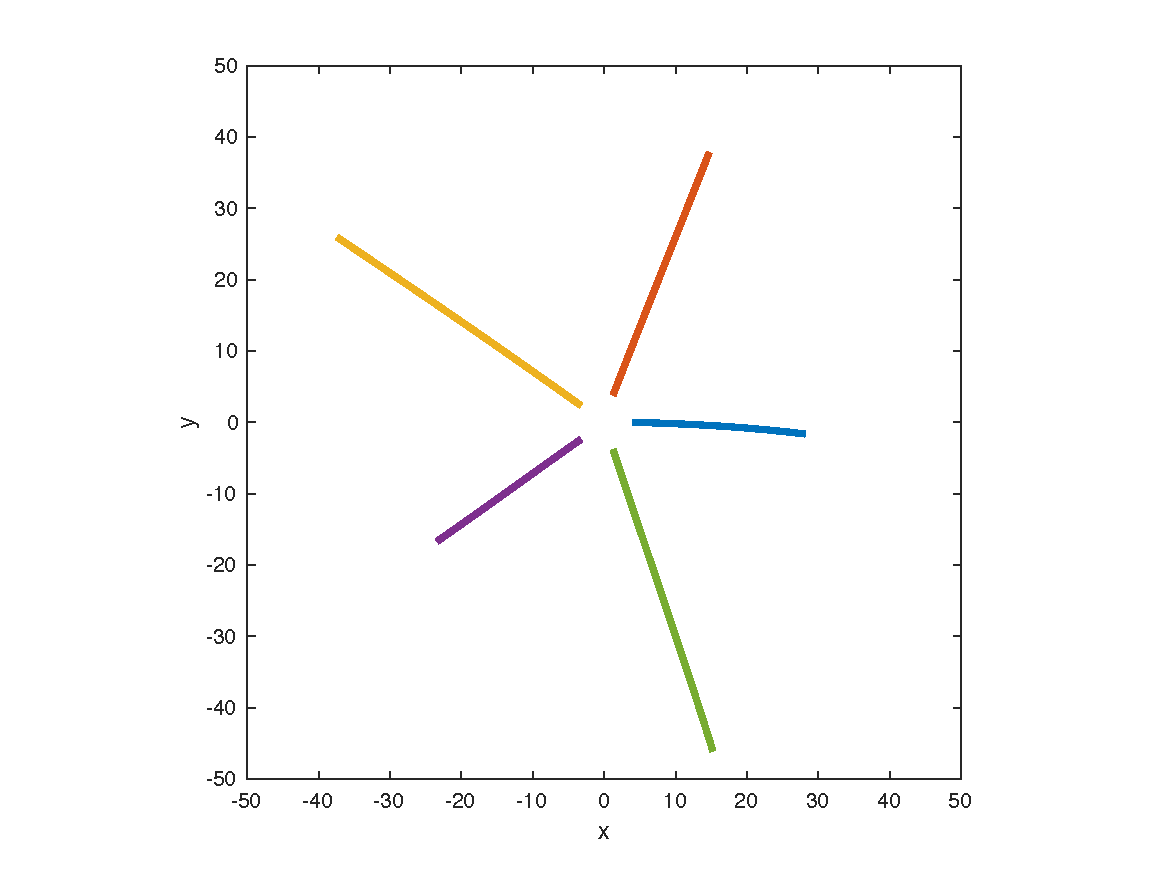
\includegraphics[width =0.24 \columnwidth]{trajectory2copy.pdf}
% \hspace{-6mm}
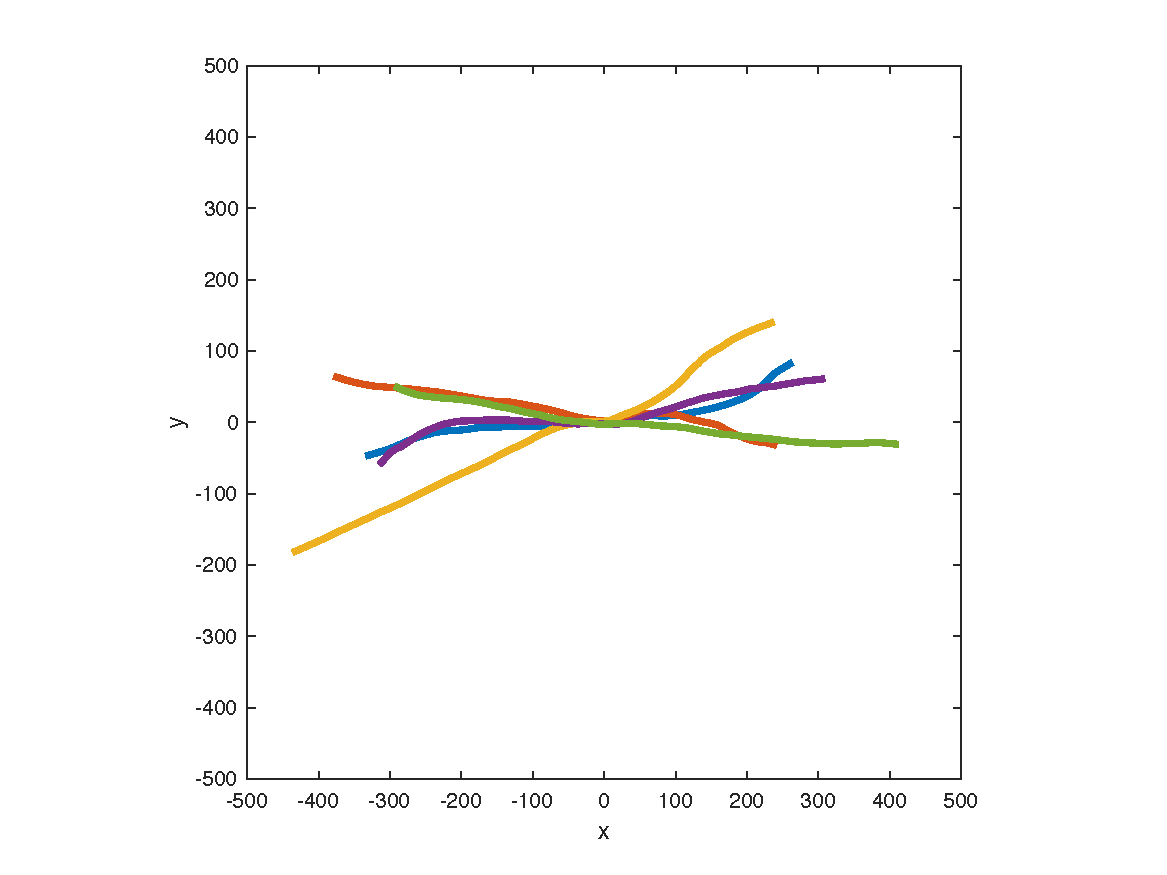
\includegraphics[width =0.24 \columnwidth]{trajectory3copy.pdf}
% \hspace{-6mm}
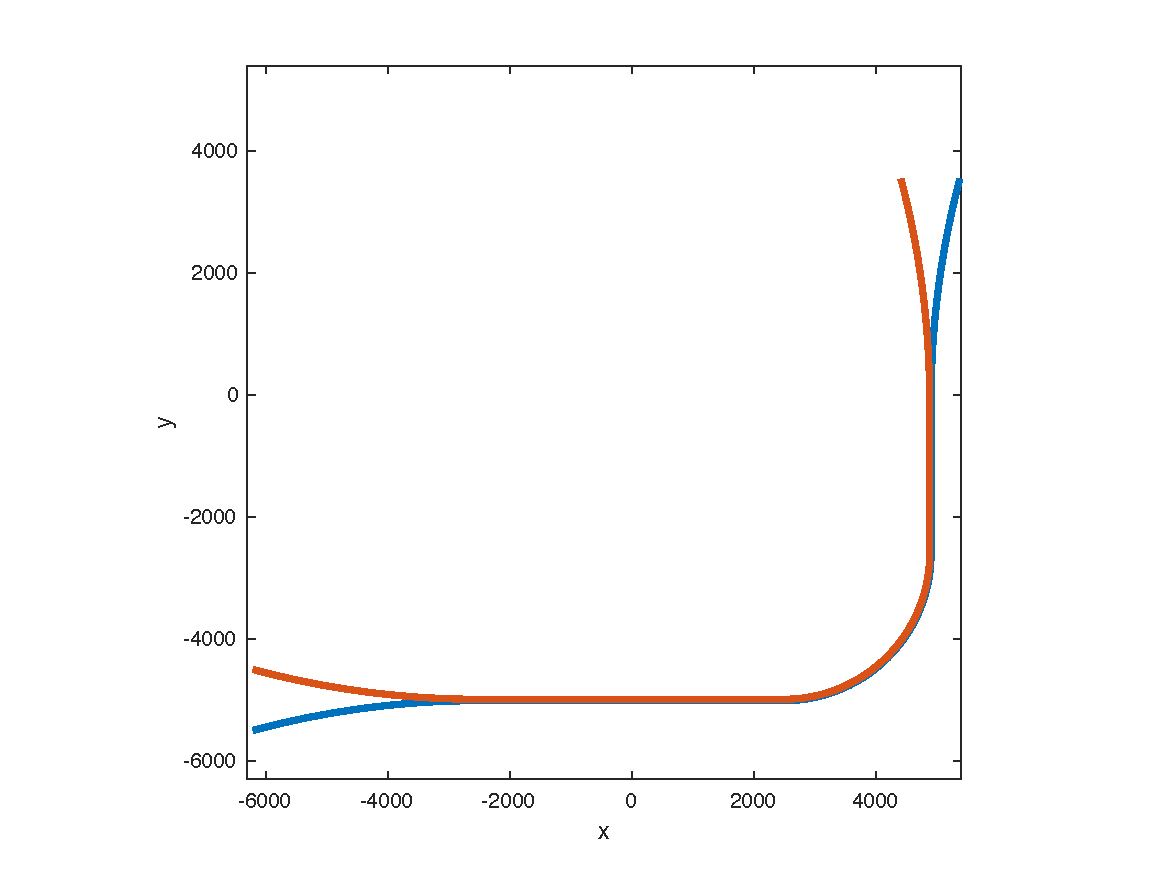
\includegraphics[width =0.24 \columnwidth]{trajectory4copy.pdf}
\caption{True target trajectories of four scenarios, from left to right: 1) 27 targets, 2) dense birth, 3) merge/split and 4) nonlinear manoeuvre.}
\label{fig:trajectory}
\end{figure}

\begin{table*}[!t]
\caption{Simulation results: go--gospa; le--location error; me--missed detection error; fe--false detection error}
\label{tab:SimulationResults}
    \centering
    \resizebox{\textwidth}{!}{%
    \begin{tabular}{c | cccc | cccc | cccc |cccc}
    & \multicolumn{4}{c|}{Scen. 1: 27 targets} & \multicolumn{4}{c|}{Scen. 2: dense birth} & \multicolumn{4}{c|}{Scen. 3: merge/split} & \multicolumn{4}{c}{Scen. 4: non-lin. man.}\\
    Filter & \textsc{ go } & \textsc{ le } & \textsc{ me } & \textsc{ fe } & \textsc{ go } & \textsc{ le } & \textsc{ me } & \textsc{ fe } & \textsc{ go } & \textsc{ le } & \textsc{ me } & \textsc{ fe }  & \textsc{ go } & \textsc{ le } & \textsc{ me } & \textsc{ fe }\\
    \hline
    \textsc{pmbm w/o merging}                              & $7.38$ & $0.56$ & $0.40$ & $1.69$ & $13.51$ & $\mathbf{1.30}$ & $6.44$ & $1.34$ & $\mathbf{22.08}$ & $\mathbf{1.14}$ & $\mathbf{12.89}$ & $4.28$ & $\mathbf{5.97}$ & $\mathbf{2.79}$ & $\mathbf{0.36}$ & $\mathbf{0.12}$\\
    \textsc{pmbm w/ merging}          & $7.18$ & $0.56$ & $0.26$ & $1.67$ & $\mathbf{13.44}$ & $\mathbf{1.30}$ & $\mathbf{6.38}$ & $1.30$ & $22.53$ & $1.26$ & $13.24$ & $\mathbf{3.86}$ & $7.45$ & $2.98$ & $1.31$ & $0.48$ \\
    \textsc{to-pmb} & $7.03$ & $0.56$ & $0.23$ & $1.55$ & $13.78$ & $1.34$ & $6.55$ & $1.30$ & $23.75$ & $1.38$ & $13.67$ & $4.10$ & $10.29$ & $3.28$ & $3.32$ & $1.16$\\
    \textsc{mla-pmb}                            & $7.00$ & $0.56$ & $0.19$ & $1.57$ & $13.58$ & $1.32$ & $6.48$ & $\mathbf{1.24}$ & $23.19$ & $1.34$ & $13.55$ & $3.9$ & $9.88$ & $3.26$ & $2.98$ & $1.06$\\
    \textsc{eafs-pmb}                            & $\mathbf{6.96}$ & $0.56$ & $\mathbf{0.19}$ & $\mathbf{1.52}$ & $13.68$ & $1.33$ & $6.55$ & $1.26$ & $23.05$ & $1.31$ & $13.43$ & $3.95$ & $9.75$ & $3.23$ & $2.92$ & $1.03$
    \end{tabular}
    }
\end{table*}

In the first scenario, 27 randomly generated targets are born from four localized positions, and they appear in and disappear from the surveillance area at different time steps. The parameters were set to $p^D = 0.90, p^S = 0.99$ and $ \lambda = 60$. This scenario illustrates how the different filters behave with a high target number and high clutter density scenario. In the second scenario, five targets are born at a very short distance from each other at the same time step. The parameters were set to $p^D = 0.90, p^S = 0.99$ and $ \lambda = 20$. This scenario tests different filters capabilities of handling a dense birth. In the third scenario, five targets first get close to each other and then separate. The parameters were set to $p^D = 0.75, p^S = 0.99$ and $ \lambda = 30$. This scenario tests different filters capabilities of handling coalescence under low detection probability. In the fourth scenario, two targets first get close, and then they maneuver in close proximity before splitting. The parameters were set to $p^D = 0.98, p^S = 0.99$ and $ \lambda = 10$. Here, the data association is very challenging due to the coalescence and the highly-nonlinear motion when targets are turning.

% The scenario parameters clutter rate $\lambda$, detection probability $p^D$ , and survival probability $p^S$ are summarised in Table \ref{tab:SimulationParameters}.

\begin{table}[!t]
\caption{Average time $[s]$ to run one full Monte Carlo simulation}
\label{tab:CycleTimes}
	\centering
	\resizebox{\columnwidth}{!}{%
	\begin{tabular}{c | c c c c c}
		Scen & PMBM & PMBM w/ Merging & TO-PMB & MLA-PMB & EAFS-PMB\\
		\hline
		1 & $178.0$ & $57.6$ & $41.6$ & $37.9$ & $41.1$ \\
		2 & $260.2$ & $45.8$ & $7.4$ & $7.7$ & $8.4$ \\
		3 & $460.4$ & $154.6$ & $51.3$ & $52.3$ & $53.1$\\
		4 & $182.5$ & $41.4$ & $23.1$ & $23.1$ & $24.8$
	\end{tabular}
	}
\end{table}

The GOSPA performance of different filters is shown in Table \ref{tab:SimulationResults}, and the average times to run a single Monte Carlo trial of the four scenarios are given in Table \ref{tab:CycleTimes}. The PMB filter with variational approximation has better estimation performance than the TO-PMB filter, especially in the scenarios with coalescence. The two variants of the PMB filter with variational approximation showed very similar performance in these four scenarios. The PMB filter has lower computational complexity than the PMBM filter, and the difference of average running time is most distinct in the second and the third scenario, where multiple targets move in close distance over a certain period of time. But the PMBM filter is able to produce better target location and extent estimations than the PMB filter, especially in the scenarios with coalescence. 

In the fourth scenario with two targets maneuvering in parallel, the process noise covariance $Q_k$ is set to a very small value. Considering that the target motion is highly non-linear while it is turning, and that small process noise only adds little uncertainty to the prediction, a too small $Q_k$ can make the data association even more challenging. We have also evaluated the same case but with a correctly chosen $Q_k$. Empirically, we found that both the PMBM filter and the PMB filter can yield equally good results. In all the simulated scenarios, the measurement noise covariance $R_k$ is set to zero. Typically, more measurement noise will result in a more challenging tracking problem. We have studied the influence of measurement noise on the PMBM and the PMB filters, but the empirical results did not show any more interesting difference between different filters compared to the case with zero measurement noise. 

% \begin{figure*}[t!]
%     \centering
%     \subfloat[][27 targets]{
%         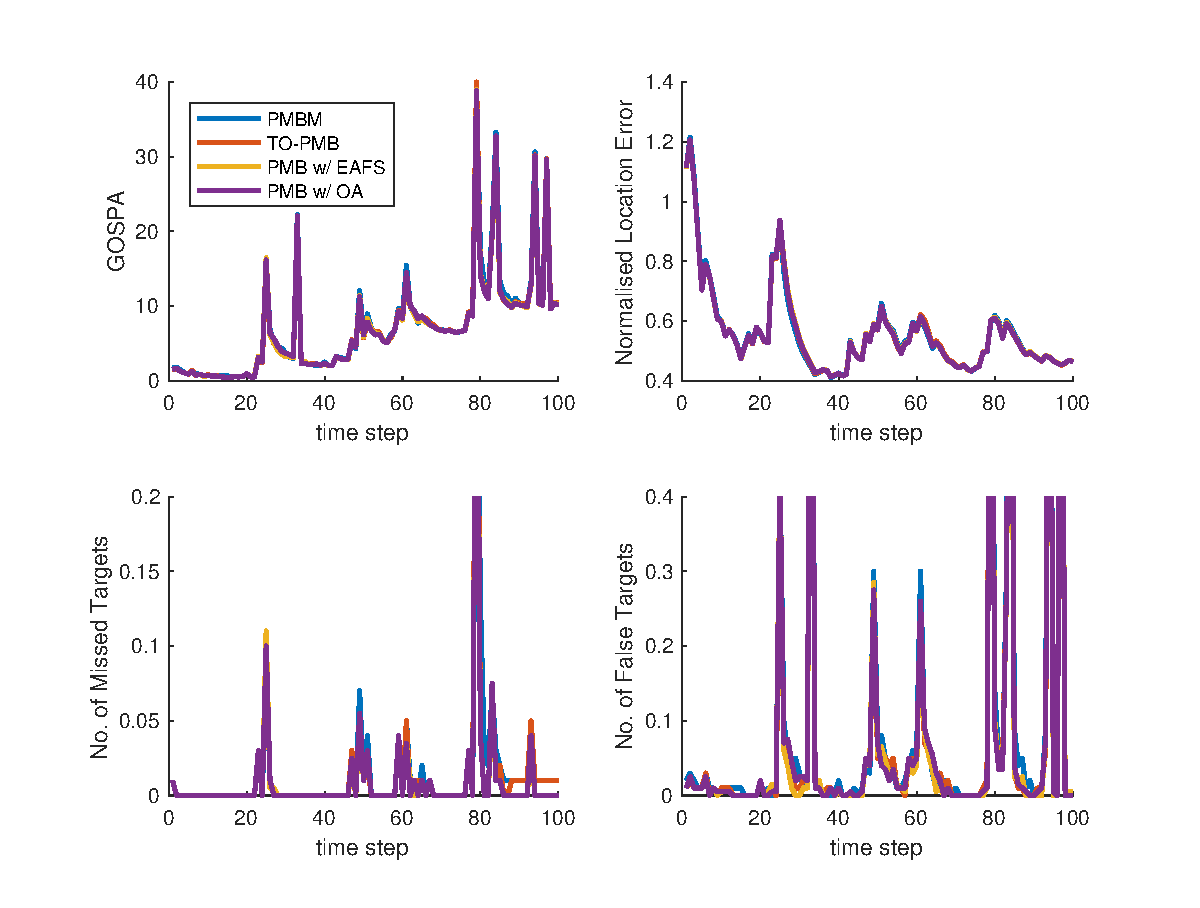
\includegraphics[width = 0.99 \columnwidth]{GOSPA27Targets.eps}}
%     \subfloat[][Dense birth]{
%         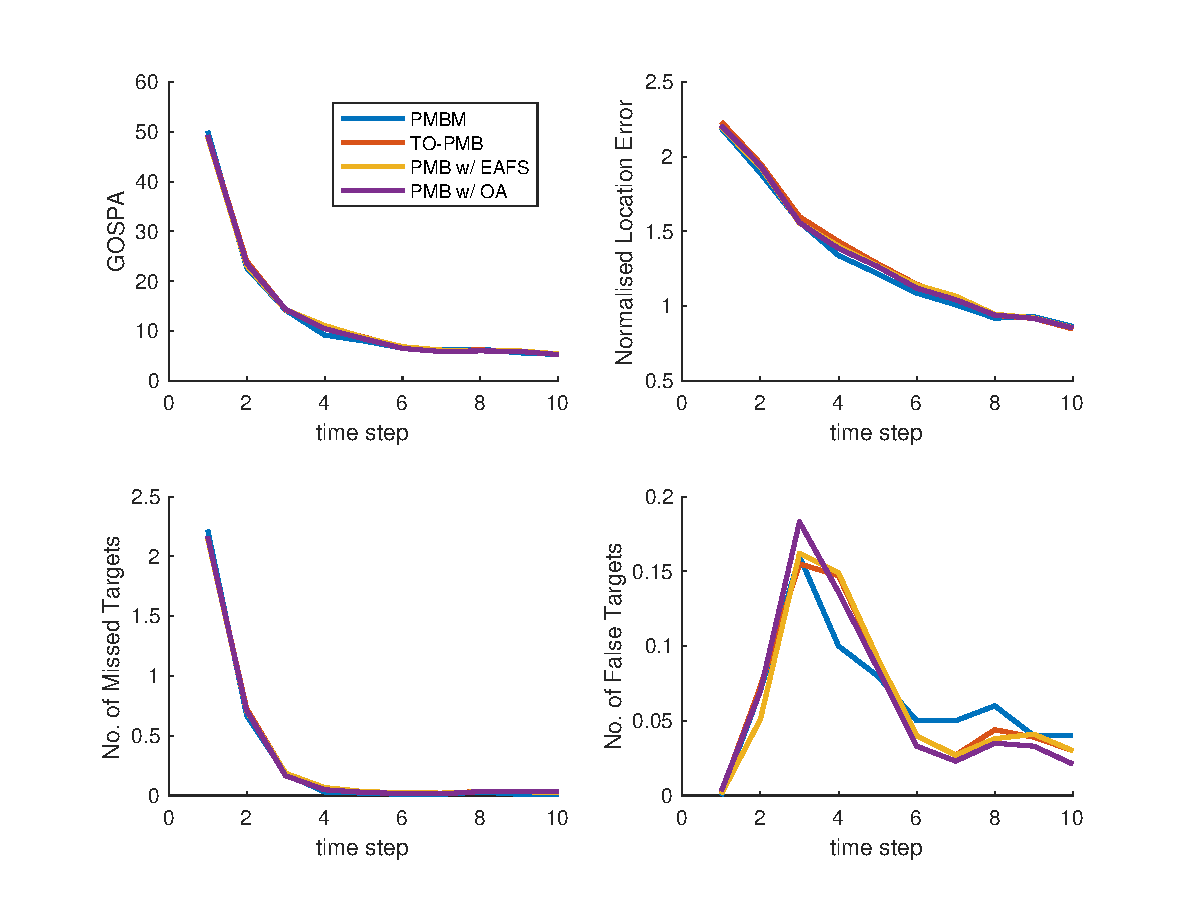
\includegraphics[width = 0.99 \columnwidth]{GOSPAdenseBirth.eps}}
%         \\
%     \subfloat[][Merge/split]{
%         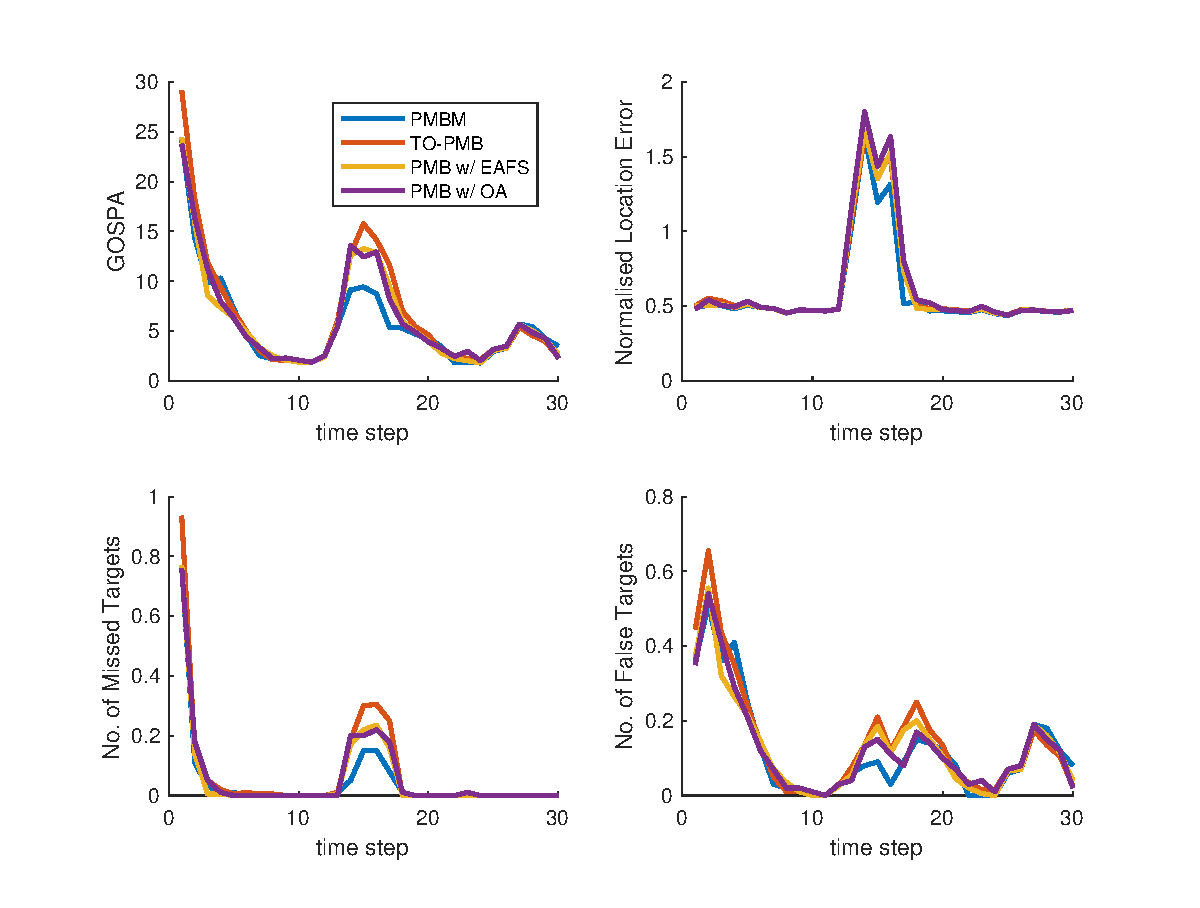
\includegraphics[width = 0.99 \columnwidth]{GOSPAmergeSplit.eps}}
%     \subfloat[][Parallel manoeuvre]{
%         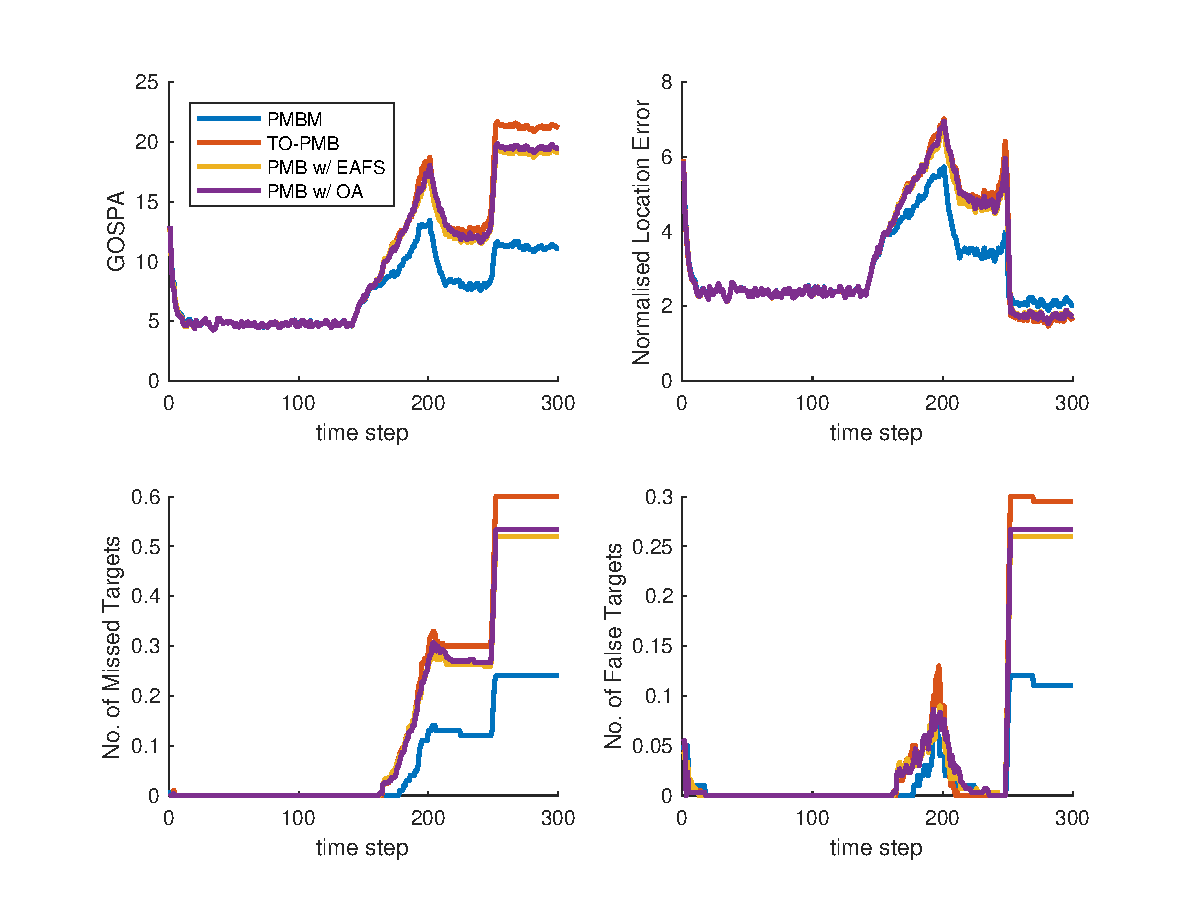
\includegraphics[width = 0.99 \columnwidth]{GOSPAparallelTurn.eps}}
%     \caption{Results from simulation of four different scenarios.}%Overall \textsc{mhg} and \textsc{so} have best performance.
% 	\label{fig:SimulationResults}
% \end{figure*}
% True target trajectories for the three simulated scenarios. In scenario 1 (left), 27 targets are born from four localised positions, and they appear and disappear the area at different time steps. In scenario 2 (centre), five targets are born from roughly the same position at the same time. In scenario 3 (right), two targets first get close, and then they manoeuvre next to each other before splitting.



% \begin{table}
% \caption{Simulation scenario parameters}
% \label{tab:SimulationParameters}
% 	\centering
% 	\begin{tabular}{c | l l l}
% 		Scenario & $\lambda$ & $p^D$ & $p^S$\\
% 		\hline
% 		1 & $60$ & $0.90$ & $0.99$ \\
% 		2 & $20$ & $0.90$ & $0.99$ \\
% 		3 & $10$ & $0.98$ & $0.99$
% 	\end{tabular}
% \end{table}

\section{Conclusions}
This paper has proposed a tractable and efficient extended target filtering algorithm based on an approximation of a PMBM posterior density.. A simulation study shows that the proposed PMB filter retains the advantage of the PMBM filter but with lower computational complexity. Possible future work includes how to improve the estimation of target extent and how to incorporate the formation of new tracks in the variational MB algorithm. 


% The goal of the variational MB algorithm presented in \cite{variational} is to obtain the best-fitting MB $g(\mathbf{X})$ that minimizes the set KL divergence from the MBM distribution $f(\mathbf{X})$:
% \begin{equation}
% \underset{g}{\arg\min}\int f(\mathbf{X})\log\frac{f(\mathbf{X})}{g(\mathbf{X})} = \underset{g}{\arg\max}\int f(\mathbf{X})\log g(\mathbf{X})\delta\mathbf{X}.
% \label{eq:kl}
% \end{equation}
% Minimising the KL divergence (\ref{eq:kl}) analytically is difficult. An approximate solution of (\ref{eq:kl}) is based on minimizing the upper bound of the true objective, following a similar process to expectation-maximization \cite{em}. The correspondence between the underlying Bernoulli distribution in $f(\mathbf{X})$ and the Bernoulli component in the best-fitting distribution $g(\mathbf{X})$ is treated as missing data $q(\cdot)$. Note that , in the point target PMB filter, each measurement creates a new track, hence each MB density in the updated MBM has equal number of Bernoulli components. 

% An approximated upper bound to the objective of (\ref{eq:kl}) is given by \cite{variational}
% \begin{multline}
% D_{\text{UB}}(f(\mathbf{X})||g(\mathbf{X}))= -\sum_{j\in\mathbb{J},\pi\in\Pi^j_N}\mathcal{W}^jq^j(\pi^j)\\\times\sum_{i=1}^N\int f^{j,\pi^j(i)}(\mathbf{X})\log g^{i}(\mathbf{X})\delta \mathbf{X},
% \label{eq:vaorigin}
% \end{multline}
% where $N$ denotes the number of Bernoulli components in each MB of $f(\mathbf{X})$ and the approximated MB $g(\mathbf{X})$; $\Pi^j_N$ is the set of all ways to assign the Bernoulli components in the $j$th MB $f^j(\mathbf{X})$ to the Bernoulli components in $g(\mathbf{X})$; the missing data $q^j(\pi^j)$ is constrained to vary only with the $j$th MB, and it satisfies $q^j(\pi^j)\geq0$ and  $\sum_{\pi^j\in\Pi^j_N} q^j(\pi^j) = 1$. The standard method for solving the form of (\ref{eq:vaorigin}) is by block coordinate descent, which alternates between minimisation with respect to $g^i(\mathbf{X})$ (M-step) and $q_j(\pi^j)$ (E-step) \cite{variational}. Because solving the above problem suffers from combinatorial complexity, approximation is needed to obtain a tractable solution.


% \appendices
% \section{Proof of Theorem \ref{theorem1}}
% \label{appendix:proof}
% In this appendix, we prove Theorem \ref{theorem1}. To simplify notation, the time index will be removed. The minimization problem of (\ref{eq:joingMBkl}) can be reformulated as
% \begin{multline}
% \underset{g^{o},g^{n}}{\arg\min} - \sum_{j\in\mathbb{J}} \mathcal{W}_j \int  \sum_{\setX^o \uplus \setX^n = \setX^d } f^{j,o} (\setX^o) f^{j,n} (\setX^n) \\\times\log \left( \sum_{\hat\setX^o \uplus \hat\setX^n = \setX^d } g^{o}(\hat\setX^o) g^{n} (\hat\setX^n) \right) \delta \setX \label{eq:KLdivMaxProblem}
% \end{multline}
% According to \cite[Lemma 2]{variational}, we can rewrite the objective function of the minimization problem \eqref{eq:KLdivMaxProblem} as
% \begin{multline}
%     J([g^o,g^n]) =  - \sum_{j\in\mathbb{J}} \mathcal{W}_j \iint f^{j,o} (\setX^o) f^{j,n} (\setX^n) \\\times\log \left( \sum_{\hat\setX^o \uplus \hat\setX^n = \setX^o \uplus \setX^n } g^{o}(\hat\setX^o) g^{n} (\hat\setX^n) \right) \delta \setX^{o}\delta\setX^{n}.
% \end{multline}
% Now, we use the log-sum inequality, where the permutation weight $q(\pi)$ is chosen such that $q(\pi) = 1$ if $\hat\setX^o = \setX^o$ and $\hat\setX^n = \setX^n$, and zero otherwise. This gives us
% \begin{align}
%     J([g^o,g^n]) &\leq - \sum_{j\in\mathbb{J}} \mathcal{W}_j \iint f^{j,o} (\setX^o) f^{j,n} (\setX^n) \\&~~~~~\times\log \left( g^{o}(\setX^o) g^{n} (\setX^n) \right) \delta \setX^{o}\delta\setX^{n} \nonumber\\
%     & =  - \sum_{j\in\mathbb{J}} \mathcal{W}_j \bigg( \int f^{j,o} (\setX^o) \log \left( g^{o}(\setX^o) \right) \delta \setX^{o} \\&~~~~~+ \int f^{j,n} (\setX^n) \log \left( g^{n} (\setX^n) \right) \delta\setX^{n} \bigg)\nonumber \\
%     & = - \int \sum_{j\in\mathbb{J}} \mathcal{W}_j f^{j,o} (\setX^o) \log \left( g^{o}(\setX^o) \right) \delta \setX^{o} \\&~~~~~- \int \sum_{j\in\mathbb{J}} \mathcal{W}_j f^{j,n} (\setX^n) \log \left( g^{n} (\setX^n) \right) \delta\setX^{n}\nonumber.
% \end{align}
% The objective function in the minimization problem \eqref{eq:KLdivMaxProblem} has an upper bound that, when we minimize over $g^o(\cdot)$ and $g^n(\cdot)$, can be broken down into two separate minimization problems
% \begin{align}
%     & \min_{g^o,g^n} \Bigg[ - \int \sum_{j\in\mathbb{J}} \mathcal{W}_j f^{j,o} (\setX^o) \log \left( g^{o}(\setX^o) \right) \delta \setX^{o} \\&~~~~~- \int \sum_{j\in\mathbb{J}} \mathcal{W}_j f^{j,n} (\setX^n) \log \left( g^{n} (\setX^n) \right) \delta\setX^{n} \Bigg] \nonumber \\
%     & = \min_{g^o} \left[- \int \sum_{j\in\mathbb{J}} \mathcal{W}_j f^{j,o} (\setX^o) \log \left( g^{o}(\setX^o) \right) \delta \setX^{o} \right] \\&~~~~~+ \min_{g^n} \left[ - \int \sum_{j\in\mathbb{J}} \mathcal{W}_j f^{j,n} (\setX^n) \log \left( g^{n} (\setX^n) \right) \delta\setX^{n} \right]\nonumber
% \end{align}
% Note that the arguments that minimize these two objective functions are the same as the arguments that minimize the KL divergences,
% \begin{align}
%     & \underset{g^{o}}{\arg\min} D\bigg( \sum_{j\in\mathbb{J}} \mathcal{W}_j f^{j,o} (\setX^o) || g^o(\setX^o)  \bigg), \\
%     & \underset{g^{n}}{\arg\min} D\bigg( \sum_{j\in\mathbb{J}} \mathcal{W}_j f^{j,n} (\setX^n) || g^n(\setX^n) \bigg).
% \end{align}
% This proves Theorem \ref{theorem1}.

% \section{Cross Entropy between Two Bernoulli-GGIWs}
% \label{appendix:crossentropy}
% Suppose $f^h(\mathbf{X})$ and $g^i(\mathbf{X})$ are two Bernoulli process with the following form
% \begin{subequations}
% \begin{align}
%     f^{h}(\mathbf{X}) &= \begin{cases}
%         1 - r^{h} & \mathbf{X} = \emptyset,\\
%         r^{h}\mathcal{GGIW}(\mathbf{x}^{h};\zeta^{h}) & \mathbf{X} = \{\mathbf{x}\},
%     \end{cases}\\
%     g^{i}(\mathbf{X}) &= \begin{cases}
%         1 - r^{i} & \mathbf{X} = \emptyset,\\
%         r^{i}\mathcal{GGIW}(\mathbf{x}^{i};\zeta^{i}) & \mathbf{X} = \{\mathbf{x}\}.
%     \end{cases}
% \end{align}
% \end{subequations}
% The cross entropy between $f^h(\mathbf{X})$ and $g^i(\mathbf{X})$ can be expressed as:
% \begin{multline}
%     -\int f^{h}(\mathbf{X})\log g^{i}(\mathbf{X})\delta\mathbf{X} = -(1-r^{h})\log(1-r^i) \\- r^{h}\log r^i - r^{h}\bigg(\int\mathcal{N}(\xi^{h};m^{h},P^{h})\log\mathcal{N}(\xi^i;m^i,\hat{P}^i)d\mathbf{x} \\+ \int\mathcal{GAM}(\gamma^{h};a^{h},b^{h})\log\mathcal{GAM}(\gamma^i;a^i,b^i)d\mathbf{x} \\+ \int\mathcal{IW}(\chi^{h};v^{h},V^{h})\log\mathcal{IW}(\chi^i;v^i,V^i)\delta\mathbf{x} \bigg),
% \end{multline}
% where
% \begin{subequations}
% \begin{multline}
%     \int\mathcal{N}(\xi^{h};m^{h},P^{h})\log\mathcal{N}(\xi^i;m^i,P^i)d\mathbf{x} =\\ -\frac{d}{2}\log(2\pi)-\frac{1}{2}\log|P^i|\\-\frac{1}{2}\text{Tr}\bigg(\big(P^{h}+(m^{h}-m^i)(m^{h}-m^i)^T\big)\big(P^i\big)^{-1}\bigg),
%     \end{multline}
%     \begin{multline}
%         \int\mathcal{GAM}(\gamma^{h};a^{h},b^{h})\log\mathcal{GAM}(\gamma^i;a^i,b^i)d\mathbf{x} = a^i\log b^i \\- \log\Gamma(a^i) + (a^i-1)(\psi_0(a^{h})-\log b^{h}) - b^i\frac{a^{h}}{b^{h}},
%     \end{multline}
%     % \text{and}
%     \begin{multline}
%         \int\mathcal{IW}(\chi^{h};v^{h},V^{h})\log\mathcal{IW}(\chi^i;v^i,V^i)d\mathbf{x} =\\ -\frac{(v^i-d-1)d}{2}\log2 + \frac{v^i-d-1}{2}\log|V^i| \\- \log\Gamma_d\bigg(\frac{v^i-d-1}{2}\bigg) - \frac{v^i}{2}\bigg(\log|V^{h}|-d\log2\\-\sum_{j=1}^d\psi_0\bigg(\frac{v^{h}-d-j}{2}\bigg)\bigg) -\frac{1}{2}\text{Tr}\big((v^{h}-d-1)(V^{h})^{-1}V^i\big).
%     \end{multline}
% \end{subequations}


\bibliographystyle{IEEEtran}
\bibliography{IEEEabrv,mybibli}


\end{document}
